% Plain-language review document (explaneat plain-language review), v5.
\documentclass[a4paper,10pt]{article}
\usepackage[margin=1.8cm]{geometry}
\usepackage{amsmath}
\usepackage{amssymb}
\usepackage{booktabs}
\usepackage{tabularx}
\usepackage{graphicx}
\usepackage[table,usenames,dvipsnames]{xcolor}
\usepackage{tikz}
\usetikzlibrary{arrows.meta,fit,backgrounds,positioning,calc}
\usetikzlibrary{shapes.geometric}
\usepackage{longtable}
\usepackage{pdflscape}
\usepackage{float}
\usepackage[font=small,labelfont=bf]{caption}
\usepackage{array}
\usepackage[unicode=true,hidelinks]{hyperref}
\setcounter{tocdepth}{3}
\setcounter{secnumdepth}{3}
% Review markers, copied from dissertation.tex (7 Nov 2026) for standalone builds.
\newif\ifreviewmarks
\reviewmarkstrue
\newcommand{\reviewrule}{\noindent{\color{BrickRed}\rule{\linewidth}{0.8pt}}}
\newenvironment{drafted}[1][]{%
  \ifreviewmarks\par\addvspace{\medskipamount}\reviewrule\par\nopagebreak
  \noindent{\color{BrickRed}\sffamily\footnotesize\textbf{Thesis Draft}\quad #1\hfill review}\par\nopagebreak\smallskip\fi}{%
  \ifreviewmarks\par\smallskip\noindent{\color{BrickRed}\sffamily\footnotesize end of thesis draft}\par\nopagebreak\reviewrule\par\medskip\fi}
\newcommand{\figreview}[1]{\ifreviewmarks\par\smallskip{\color{NavyBlue}\sffamily\footnotesize\textbf{Figure note:} #1}\par\fi}
\begin{document}
\begin{center}{\Large\bfseries Plain-language explanation: churn100-s4-c2\par}\vspace{2mm}{\small AI-assisted drafts for review. Nothing here has been verified by a person.\par}\end{center}
\noindent\textbf{How to read this.} Explanations are built up but read down: the summary first, then each part from the whole model down, in plain words, each sentence followed by the claims it rests on (C01, C02, \ldots; every cited claim was computed on the model and checked). Numbers are changes in predicted risk for a typical patient. The technical record (original hypotheses, formulas, evidence tables with the test check, ranges and n) is at the end. The text describes what the model does, not the world; whether it is plausible is for the reviewer to judge.
\par\medskip\noindent\textbf{What changed in v5e (figures).} v5e: every diagram is a numbered figure with a caption (list of figures after the contents) and the text refers to it; the whole-network figure has its own landscape page, scaled to the page, with a short caption and its description in the text; an input used by several parts is drawn under each of them (same input, repeated for readability, dotted outline); and an appendix figure shows the trained network before any explanation (no parts, no splits).
\par\medskip\noindent\textbf{What changed in v5c (tables and diagrams).} v5c: the evidence tables are landscape, compact and shaded by row, with the header repeated on every page (longtable and pdflscape, used in this review PDF only; the thesis preamble has neither). In the diagrams each input is drawn once, in a shared row along the bottom (the explanation's split copies of an input are listed in the technical detail instead), every cluster has one output rectangle with its plain name, the inputs that feed the output directly meet in a drawn 'sum', and a one-line legend explains the edges.
\par\medskip\noindent\textbf{What changed in v5b (diagrams).} v5b uses one grouping everywhere, the annotation hierarchy: the summary's diagram is the same picture as the whole model's section, and a part that is itself a weighted sum (blood pressure with cholesterol) is a part of its own, described as one that adds up, so the text counts three parts throughout; the lint checks every 'N parts' against the hierarchy. A full-structure diagram follows the summary: every node and connection, nested by part, with the inputs that feed the output directly in their own cluster and the unused input columns listed. Each section from the top down adds its own region of that diagram, with stubs for connections from or to other parts; each connection is drawn in exactly one section. The gate's text now says that it lowers the risk for the patients it acts on, and that more vessels and higher cholesterol take that lowering away; its vessel statements are one per group.
\par\medskip\noindent\textbf{What changed in v5 (read down).} v5 reads the explanation down. The summary (one line, a diagram, one paragraph per block) is as in v4, except that the paragraph on what adds up is split into protective items, risk-raising items and rare results, and an input that also feeds a part is quoted with its direct contribution only (the rest is in that part's paragraph). Then the document walks the annotation hierarchy from the whole model down: for each part a plain hypothesis (what it does for the prediction), plain evidence (what was checked and what it showed; for a part made of others, what they are and how they combine), a diagram one level down and where to read on. The original hypotheses, closed forms and evidence tables are in 'Technical detail' at the end. Statements about structure (what a part is made of, a copy of another part, a formula that reproduces it) are now claims of their own, checked on the graph and the data.
\par\medskip\noindent\textbf{v4.} v4 follows the structure of the explanation. The summary opens with one line and a diagram at the same grouping, then gives one paragraph per top-level block of the annotation hierarchy: one for everything that adds up independently (the inputs that feed the model score directly, and parts that are a weighted sum), and one for each part that combines its inputs in another way: what it combines, how, and for whom. 'Parts in detail' follows the hierarchy below that, with a diagram one level down for each part that contains others. The prose no longer says 'clearly', 'slightly', 'consistently' or 'on the training data only': the numbers carry it, and the test check, the ranges and n stay in the evidence tables. Only genuinely small groups are marked, with their n. The lint rejects the confidence words and checks the block structure.
\tableofcontents
\listoffigures
\clearpage
\begin{drafted}[plain-language layer: churn100-s4-c2]
\section{churn100-s4-c2}
\noindent{\small Genome \texttt{4206744f-b5ce-4488-bc53-a39aa08fe972}, explanation \texttt{33d6db5d-fbdf-41c8-a597-fc997715b92f}. Split: train primary (n=4000), test as a check (n=1000). Claims: 113, verified 110, not supported 3.\par}
\noindent{\small\textcolor{BrickRed}{AI-assisted draft for review (unverified)}\par}\smallskip
\noindent{\footnotesize Reference (typical) customer: the typical customer: the median training customer for every number and the most common training category for every category (not a real customer). account length: 100; area code: area code 415; international plan: no international plan; number customer service calls: 1 calls; number vmail messages: 0 messages; state: West Virginia; total day calls: 100 calls; total day charge: 30.69 US dollars; total day minutes: 180 minutes; total eve calls: 100 calls; total eve charge: 17.12 US dollars; total eve minutes: 201 minutes; total intl calls: 4 calls; total intl charge: 2.78 US dollars; total intl minutes: 10 minutes; total night calls: 100 calls; total night charge: 9.02 US dollars; total night minutes: 200 minutes; voice mail plan: no voice-mail plan. Predicted chance that a customer leaves: 3\%.\par}
\subsection{Summary}
\noindent For a typical customer (in West Virginia, area code 415, no international or voice-mail plan, no voice-mail messages, 1 call to customer service and median usage) the model predicts a chance of leaving of about 3\%; it adds up six parts: fixed-weight inputs, service calls, heavy daytime use, state units, an evening unit and a small voice-mail unit.\,{\scriptsize\textcolor{NavyBlue}{[C046]}} Figure~\ref{fig:churn100s4c2:summary} shows the model at this level: one box per paragraph below.
\par\medskip\noindent\fbox{\begin{minipage}{0.96\linewidth}\small\textbf{How to read the diagrams.} Edge colour is the sign of that one connection: blue positive, red negative; thicker is a larger weight. The outline and arrow on an input (and on a part's output box) is its overall effect on the final prediction, read from the verified claims: orange and up arrow raises it, teal and down arrow lowers it, grey and double arrow depends (it goes both ways, or differs between levels). A negative connection into a part that itself raises the prediction means that input lowers the prediction; through a hinge the overall effect can only be read from the claims, not from the edges. Up arrow means towards churn; down arrow, away from it. A double outline marks an input (or a part's output) that acts at a fixed rate everywhere: it adds the same amount to the score per unit, so it is explained by its rate alone (see 'Linear factors'); a dashed double outline, at a fixed rate on the observed data. The normal outline is an input whose effect switches on and off somewhere. For example, a voice-mail plan has a negative connection into 'Fixed-weight inputs', a part that raises the predicted chance that a customer leaves, so a voice-mail plan lowers it.\end{minipage}}\par\medskip
\begin{figure}[H]\centering
\resizebox{!}{\ifdim\height>0.5\textheight 0.5\textheight\else\height\fi}{%
\resizebox{\ifdim\width>\linewidth\linewidth\else\width\fi}{!}{%
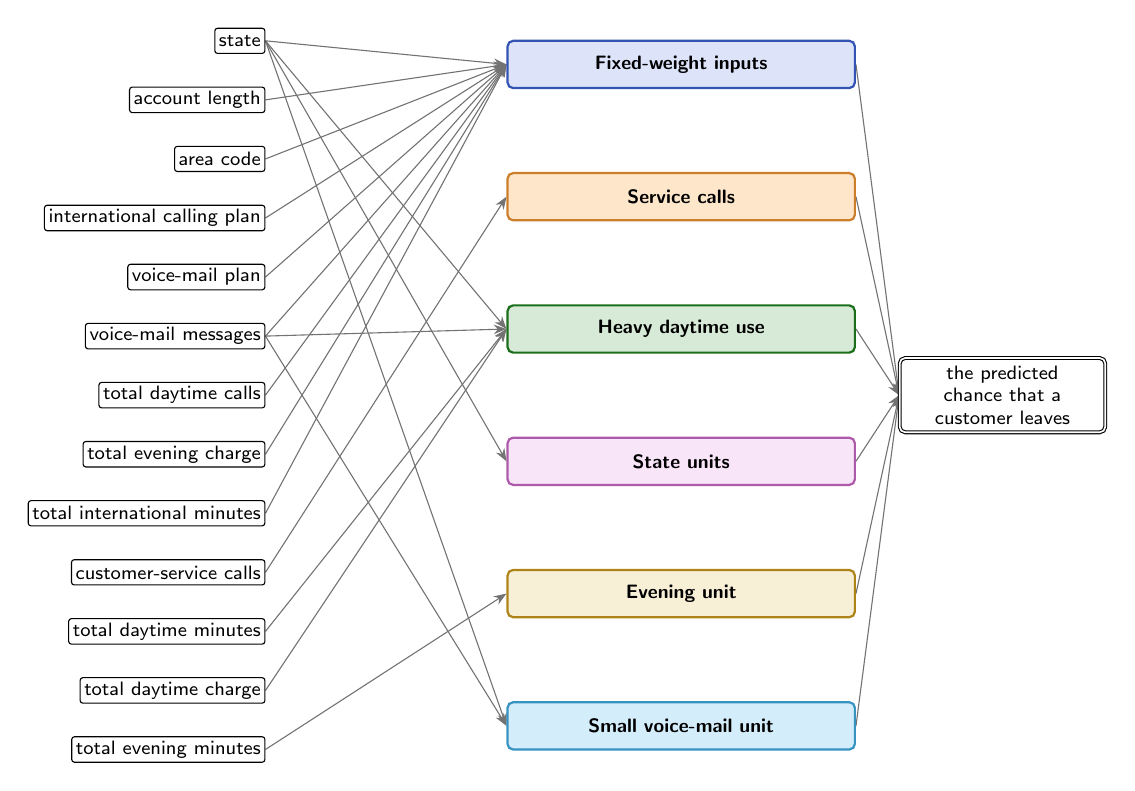
\begin{tikzpicture}[
  font=\sffamily\scriptsize, >={Stealth[length=1.6mm]},
  inp/.style={draw, rounded corners=1pt, fill=white, inner sep=1.5pt, minimum height=3.2mm, anchor=east},
  abox/.style={draw, thick, rounded corners=2pt, align=center, inner sep=3pt, minimum height=6mm, text width=42mm},
  outp/.style={draw, double, rounded corners=2pt, fill=white, align=center, inner sep=3pt, text width=24mm},
  agg/.style={draw=black!55},
]
\node[inp] (i0) at (0,4.5) {state};
\node[inp] (i1) at (0,3.75) {account length};
\node[inp] (i2) at (0,3.0) {area code};
\node[inp] (i3) at (0,2.25) {international calling plan};
\node[inp] (i4) at (0,1.5) {voice-mail plan};
\node[inp] (i5) at (0,0.75) {voice-mail messages};
\node[inp] (i6) at (0,-0.0) {total daytime calls};
\node[inp] (i7) at (0,-0.75) {total evening charge};
\node[inp] (i8) at (0,-1.5) {total international minutes};
\node[inp] (i9) at (0,-2.25) {customer-service calls};
\node[inp] (i10) at (0,-3.0) {total daytime minutes};
\node[inp] (i11) at (0,-3.75) {total daytime charge};
\node[inp] (i12) at (0,-4.5) {total evening minutes};
\node[abox, fill=RoyalBlue!18, draw=RoyalBlue!80!black] (b0) at (5.28,4.2) {\textbf{Fixed-weight inputs}};
\node[abox, fill=BurntOrange!18, draw=BurntOrange!80!black] (b1) at (5.28,2.52) {\textbf{Service calls}};
\node[abox, fill=ForestGreen!18, draw=ForestGreen!80!black] (b2) at (5.28,0.84) {\textbf{Heavy daytime use}};
\node[abox, fill=Orchid!18, draw=Orchid!80!black] (b3) at (5.28,-0.84) {\textbf{State units}};
\node[abox, fill=Goldenrod!18, draw=Goldenrod!80!black] (b4) at (5.28,-2.52) {\textbf{Evening unit}};
\node[abox, fill=Cerulean!18, draw=Cerulean!80!black] (b5) at (5.28,-4.2) {\textbf{Small voice-mail unit}};
\node[outp] (out) at (9.36,0) {the predicted chance that a customer leaves};
\begin{scope}[on background layer]
\draw[->, agg, thin] (i0.east) -- (b0.west);
\draw[->, agg, thin] (i1.east) -- (b0.west);
\draw[->, agg, thin] (i2.east) -- (b0.west);
\draw[->, agg, thin] (i3.east) -- (b0.west);
\draw[->, agg, thin] (i4.east) -- (b0.west);
\draw[->, agg, thin] (i5.east) -- (b0.west);
\draw[->, agg, thin] (i6.east) -- (b0.west);
\draw[->, agg, thin] (i7.east) -- (b0.west);
\draw[->, agg, thin] (i8.east) -- (b0.west);
\draw[->, agg] (b0.east) -- (out.west);
\draw[->, agg, thin] (i9.east) -- (b1.west);
\draw[->, agg] (b1.east) -- (out.west);
\draw[->, agg, thin] (i0.east) -- (b2.west);
\draw[->, agg, thin] (i5.east) -- (b2.west);
\draw[->, agg, thin] (i10.east) -- (b2.west);
\draw[->, agg, thin] (i11.east) -- (b2.west);
\draw[->, agg] (b2.east) -- (out.west);
\draw[->, agg, thin] (i0.east) -- (b3.west);
\draw[->, agg] (b3.east) -- (out.west);
\draw[->, agg, thin] (i12.east) -- (b4.west);
\draw[->, agg] (b4.east) -- (out.west);
\draw[->, agg, thin] (i0.east) -- (b5.west);
\draw[->, agg, thin] (i5.east) -- (b5.west);
\draw[->, agg] (b5.east) -- (out.west);
\end{scope}
\end{tikzpicture}}}%
\caption{The model at the level of the summary: one box per part.}
\label{fig:churn100s4c2:summary}
\end{figure}
\paragraph{Fixed-weight inputs.} This part adds up most inputs with fixed weights: an international plan raises a typical customer's chance of leaving from about 3\% to about 31\%, and a voice-mail plan lowers it to under 1\%.\,{\scriptsize\textcolor{NavyBlue}{[C047, C051]}} More voice-mail messages raise it steadily, from about 3\% at 0 to about 10\% at 32 messages, flattening out near the bottom because the predicted chance cannot go much lower.\,{\scriptsize\textcolor{NavyBlue}{[C049]}} A higher evening charge and more international minutes also raise it steadily, each from about 2\% to about 4\% across their usual range.\,{\scriptsize\textcolor{NavyBlue}{[C055, C056]}} Through it, the state moves the chance from about 3\% in West Virginia to about 11\% in Washington and about 7\% in New Jersey, and to under 1\% in Hawaii and in Rhode Island (72 to 122 training customers per state).\,{\scriptsize\textcolor{NavyBlue}{[C048, C050, C052, C053]}}
\paragraph{Service calls.} This part adds up two parts: a rise from 3 customer-service calls upwards and a second rise from 4 calls upwards.\,{\scriptsize\textcolor{NavyBlue}{[C079]}} From 3 calls upwards it adds to the chance slowly at first, then faster: for a typical such customer, 4 calls take it from about 3\% to about 18\%.\,{\scriptsize\textcolor{NavyBlue}{[C078]}} Up to 3 calls it barely moves a typical customer's chance, which stays at about 3\%, rising slowly at first, then faster.\,{\scriptsize\textcolor{NavyBlue}{[C077]}}
\paragraph{Heavy daytime use.} Daytime minutes add to the chance only once they rise above about 221 minutes (between 186 and 221 minutes for different customers), in an uneven way: for a typical such customer, from about 3\% at 0 minutes to about 19\% at 271 minutes.\,{\scriptsize\textcolor{NavyBlue}{[C088]}} More voice-mail messages lower it in an uneven way: for the typical customer it acts on, from about 12\% at 0 to about 6\% at 32 messages.\,{\scriptsize\textcolor{NavyBlue}{[C080]}} Customers in Washington get less from it: about 7\% instead of about 12\% for the typical customer it acts on.\,{\scriptsize\textcolor{NavyBlue}{[C082]}}
\paragraph{State units.} This part reads only the state: it raises a typical customer's chance from about 3\% to about 22\% in Rhode Island, and by less than a point in Indiana.\,{\scriptsize\textcolor{NavyBlue}{[C100, C101]}}
\paragraph{Evening unit.} This part reads evening minutes: nothing until about 217 minutes, then steadily, but a typical customer's chance stays at about 3\%.\,{\scriptsize\textcolor{NavyBlue}{[C103, C104]}}
\paragraph{Small voice-mail unit.} This small part reads voice-mail messages and being in Louisiana, and barely changes the predictions (by at most one point).\,{\scriptsize\textcolor{NavyBlue}{[C111]}}
\paragraph{The whole network.} Figure~\ref{fig:churn100s4c2:overview} (next page, landscape) draws every unit and connection of the explained model, nested by part: shaded clusters are the parts of the model and darker boxes the parts inside them; circles are hidden units (h1, h2, \ldots); each cluster's rectangle is its output, and a dashed `sum' stands for an addition the next unit does (drawn, not a unit of the model); the hexagon is the model's output. An input used by several parts is drawn under each of them (same label, dotted outline, the first copy marked with the number of copies): it is the same input, repeated for readability. Not used by the model (input columns with no connection): state: 29 of 51 levels, area code 408, area code 510, total evening calls, total night-time minutes, total night-time calls, total night-time charge, total international calls, total international charge.
\begin{landscape}
\begin{figure}[p]\centering
\resizebox{\linewidth}{!}{%
\definecolor{netup}{HTML}{D95F02}\definecolor{netdown}{HTML}{1B9E77}\definecolor{netmixed}{HTML}{7F7F7F}%
\begin{tikzpicture}[
  font=\sffamily\scriptsize, >={Stealth[length=1.4mm]},
  inp/.style={draw, circle, fill=white, minimum size=3.2mm, inner sep=0pt},
  hid/.style={draw, circle, fill=white, minimum size=5.2mm, inner sep=0.5pt, font=\sffamily\tiny},
  exitbox/.style={draw, thick, rectangle, fill=white, align=center, text width=17mm, minimum height=5mm, inner sep=1.5pt, font=\sffamily\tiny},
  sumbox/.style={draw, thick, dashed, rectangle, fill=white, align=center, text width=17mm, minimum height=5mm, inner sep=1.5pt, font=\sffamily\tiny},
  outp/.style={draw, thick, regular polygon, regular polygon sides=6, fill=white, minimum size=10mm, inner sep=0pt, font=\sffamily\tiny, align=center},
  stub/.style={draw, dashed, rounded corners=2pt, fill=white, align=center, inner sep=2pt, font=\sffamily\tiny, text width=15mm},
  inlab/.style={font=\sffamily\tiny, align=center, text width=15mm, inner sep=1pt, fill=white, fill opacity=0.8, text opacity=1},
  wpos/.style={draw=NavyBlue}, wneg/.style={draw=BrickRed}, wagg/.style={draw=black!45, line width=1.2pt},
  wmix/.style={draw=Plum},
]
\node[outp] (n0) at (22.53,7.5) {churn};
\node[hid] (n10131) at (27.59,1.9) {h9};
\node[hid] (n12171) at (18.72,3.25) {h10};
\node[hid] (n12730) at (18.72,1.9) {h11};
\node[hid] (n1295) at (33.83,1.9) {h1};
\node[hid] (n14484) at (38.42,1.9) {h12};
\node[exitbox] (n15524) at (38.42,3.25) {Evening unit $\uparrow$};
\node[hid] (n3118) at (29.09,1.9) {h2};
\node[hid] (n5268) at (18.72,4.6) {h3};
\node[exitbox] (n6089) at (43.26,1.9) {Small voice-mail unit $\uparrow$};
\node[hid] (n6713) at (14.74,3.25) {h5};
\node[hid] (n7872) at (34.58,3.25) {h6};
\node[hid] (n9436) at (14.74,1.9) {h7};
\node[hid] (n9954) at (35.33,1.9) {h8};
\node[exitbox] (nidentityxlin) at (5.85,1.9) {Fixed-weight inputs $\uparrow$};
\node[exitbox] (nidentityxsvc) at (22.2,5.95) {Service calls $\uparrow$};
\node[sumbox] (ncsumxxannx82) at (28.34,3.25) {sum: Heavy daytime use $\uparrow$};
\node[sumbox] (ncsumxxannx85) at (34.58,4.6) {sum: State units $\updownarrow$};
\node[inp, densely dotted, thick, draw=netmixed, very thick] (ngrpxxstatexxannx85) at (34.58,0.0) {};
\path (ngrpxxstatexxannx85.south) node[inlab, anchor=north] (labngrpxxstatexxannx85) {state (22 of 51 used) ($\times$4) $\updownarrow$};
\node[inp, draw=netup, very thick] (ninxxtotalxdayxminutesxxannx82) at (27.44,0.0) {};
\path (ninxxtotalxdayxminutesxxannx82.south) node[inlab, anchor=north] (labninxxtotalxdayxminutesxxannx82) {total daytime minutes $\uparrow$};
\node[inp, draw=netup, very thick] (ninxxtotalxdayxchargexxannx82) at (29.24,0.0) {};
\path (ninxxtotalxdayxchargexxannx82.south) node[inlab, anchor=north] (labninxxtotalxdayxchargexxannx82) {total daytime charge $\uparrow$};
\node[inp, draw=netup, very thick] (ninxxtotalxevexminutesxxannx83) at (38.42,0.0) {};
\path (ninxxtotalxevexminutesxxannx83.south) node[inlab, anchor=north] (labninxxtotalxevexminutesxxannx83) {total evening minutes $\uparrow$};
\node[inp, draw=netup, very thick] (ninxxnumberxcustomerxservicexcallsxxannx86) at (18.22,0.0) {};
\path (ninxxnumberxcustomerxservicexcallsxxannx86.south) node[inlab, anchor=north] (labninxxnumberxcustomerxservicexcallsxxannx86) {customer-service calls $\uparrow$};
\node[inp, densely dotted, thick, draw=netdown, very thick] (ninxxnumberxvmailxmessagesxxannx82) at (31.04,0.0) {};
\path (ninxxnumberxvmailxmessagesxxannx82.south) node[inlab, anchor=north] (labninxxnumberxvmailxmessagesxxannx82) {voice-mail messages ($\times$3) $\downarrow$};
\node[inp, densely dotted, thick, draw=netup, very thick] (ninxxnumberxvmailxmessagesxxannx84) at (44.16,0.0) {};
\path (ninxxnumberxvmailxmessagesxxannx84.south) node[inlab, anchor=north] (labninxxnumberxvmailxmessagesxxannx84) {voice-mail messages $\uparrow$};
\node[inp, densely dotted, thick, draw=netmixed, very thick] (ngrpxxstatexxannx82) at (25.64,0.0) {};
\path (ngrpxxstatexxannx82.south) node[inlab, anchor=north] (labngrpxxstatexxannx82) {state (22 of 51 used) $\updownarrow$};
\node[inp, densely dotted, thick, draw=netmixed, very thick] (ngrpxxstatexxannx84) at (42.36,0.0) {};
\path (ngrpxxstatexxannx84.south) node[inlab, anchor=north] (labngrpxxstatexxannx84) {state (22 of 51 used) $\updownarrow$};
\node[inp, densely dotted, thick, draw=netmixed, very thick] (ngrpxxstatexxannx79) at (4.5,0.0) {};
\path (ngrpxxstatexxannx79.south) node[inlab, anchor=north] (labngrpxxstatexxannx79) {state (22 of 51 used) $\updownarrow$};
\node[inp, draw=netup, very thick] (ninxxaccountxlengthxxannx79) at (1.8,-1.05) {};
\path (ninxxaccountxlengthxxannx79.south) node[inlab, anchor=north] (labninxxaccountxlengthxxannx79) {account length $\uparrow$};
\node[inp, draw=netup, very thick] (ninxxareaxcodex415xxannx79) at (3.6,-1.05) {};
\path (ninxxareaxcodex415xxannx79.south) node[inlab, anchor=north] (labninxxareaxcodex415xxannx79) {area code 415 $\uparrow$};
\node[inp, draw=netup, very thick] (ninxxinternationalxplanxxannx79) at (2.7,0.0) {};
\path (ninxxinternationalxplanxxannx79.south) node[inlab, anchor=north] (labninxxinternationalxplanxxannx79) {an international plan $\uparrow$};
\node[inp, draw=netdown, very thick] (ninxxvoicexmailxplanxxannx79) at (0.9,0.0) {};
\path (ninxxvoicexmailxplanxxannx79.south) node[inlab, anchor=north] (labninxxvoicexmailxplanxxannx79) {a voice-mail plan $\downarrow$};
\node[inp, draw=netup, very thick] (ninxxtotalxdayxcallsxxannx79) at (5.4,-1.05) {};
\path (ninxxtotalxdayxcallsxxannx79.south) node[inlab, anchor=north] (labninxxtotalxdayxcallsxxannx79) {total daytime calls $\uparrow$};
\node[inp, draw=netup, very thick] (ninxxtotalxevexchargexxannx79) at (6.3,0.0) {};
\path (ninxxtotalxevexchargexxannx79.south) node[inlab, anchor=north] (labninxxtotalxevexchargexxannx79) {total evening charge $\uparrow$};
\node[inp, draw=netup, very thick] (ninxxtotalxintlxminutesxxannx79) at (8.1,0.0) {};
\path (ninxxtotalxintlxminutesxxannx79.south) node[inlab, anchor=north] (labninxxtotalxintlxminutesxxannx79) {total international minutes $\uparrow$};
\node[inp, densely dotted, thick, draw=netup, very thick] (ninxxnumberxvmailxmessagesxxannx79) at (9.9,0.0) {};
\path (ninxxnumberxvmailxmessagesxxannx79.south) node[inlab, anchor=north] (labninxxnumberxvmailxmessagesxxannx79) {voice-mail messages $\uparrow$};
\node[font=\sffamily\tiny\bfseries, text=ForestGreen!60!black, inner sep=1pt] (subt0) at (14.74,3.75) {Calls from 4 upwards};
\node[font=\sffamily\tiny\bfseries, text=ForestGreen!60!black, inner sep=1pt] (subt1) at (18.72,5.1) {Calls from 3 upwards};
\begin{scope}[on background layer]
\node[fit=(nidentityxlin) , inner sep=8pt, rounded corners=5pt, fill=BurntOrange!10, draw=BurntOrange!45] (clu1) {};
\node[fit=(n12171) (n12730) (n5268) (n6713) (n9436) (nidentityxsvc) (subt0) (subt1), inner sep=8pt, rounded corners=5pt, fill=ForestGreen!10, draw=ForestGreen!45] (clu2) {};
\node[fit=(n10131) (n3118) (ncsumxxannx82) , inner sep=8pt, rounded corners=5pt, fill=Orchid!10, draw=Orchid!45] (clu3) {};
\node[fit=(n1295) (n7872) (n9954) (ncsumxxannx85) , inner sep=8pt, rounded corners=5pt, fill=Goldenrod!10, draw=Goldenrod!45] (clu4) {};
\node[fit=(n14484) (n15524) , inner sep=8pt, rounded corners=5pt, fill=Cerulean!10, draw=Cerulean!45] (clu5) {};
\node[fit=(n6089) , inner sep=8pt, rounded corners=5pt, fill=Mahogany!10, draw=Mahogany!45] (clu6) {};
\node[fit=(n6713) (n9436) (subt0), inner sep=4pt, rounded corners=3pt, fill=ForestGreen!26, draw=ForestGreen!70] {};
\node[fit=(n12171) (n12730) (n5268) (subt1), inner sep=4pt, rounded corners=3pt, fill=ForestGreen!26, draw=ForestGreen!70] {};
\draw[->, wneg, line width=0.60pt] (n1295) -- (ncsumxxannx85);
\draw[->, wpos, line width=0.79pt] (n3118) -- (ncsumxxannx82);
\draw[->, wpos, line width=0.25pt] (n6089) -- (n0);
\draw[->, wneg, line width=0.67pt] (n7872) -- (ncsumxxannx85);
\draw[->, wpos, line width=0.26pt] (n9954) -- (ncsumxxannx85);
\draw[->, wpos, line width=0.92pt] (n10131) -- (ncsumxxannx82);
\draw[->, wpos, line width=0.32pt] (n15524) -- (n0);
\draw[->, wpos, line width=0.44pt] (ninxxtotalxdayxminutesxxannx82) -- (n3118);
\draw[->, wpos, line width=0.38pt] (ninxxtotalxdayxchargexxannx82) -- (n3118);
\draw[->, wpos, line width=0.54pt] (ninxxtotalxdayxminutesxxannx82) -- (n10131);
\draw[->, wpos, line width=0.60pt] (ninxxtotalxevexminutesxxannx83) -- (n14484);
\draw[->, wpos, line width=0.61pt] (n1295) -- (n7872);
\draw[->, wpos, line width=0.75pt] (n9436) -- (n6713);
\draw[->, wpos, line width=0.38pt] (n12171) -- (n5268);
\draw[->, wpos, line width=0.50pt] (n12730) -- (n12171);
\draw[->, wpos, line width=0.61pt] (n14484) -- (n15524);
\draw[->, wpos, line width=0.41pt] (ninxxnumberxcustomerxservicexcallsxxannx86) -- (n9436);
\draw[->, wneg, line width=0.48pt] (ninxxnumberxvmailxmessagesxxannx82) -- (n3118);
\draw[->, wpos, line width=0.54pt] (ninxxnumberxvmailxmessagesxxannx84) -- (n6089);
\draw[->, wpos, line width=0.34pt] (ninxxnumberxcustomerxservicexcallsxxannx86) -- (n5268);
\draw[->, wpos, line width=0.55pt] (ninxxnumberxcustomerxservicexcallsxxannx86) -- (n12171);
\draw[->, wpos, line width=0.53pt] (ninxxnumberxcustomerxservicexcallsxxannx86) -- (n12730);
\draw[->, wpos, line width=0.29pt] (ninxxaccountxlengthxxannx79) -- (nidentityxlin);
\draw[->, wpos, line width=0.25pt] (ninxxareaxcodex415xxannx79) -- (nidentityxlin);
\draw[->, wpos, line width=0.54pt] (ninxxinternationalxplanxxannx79) -- (nidentityxlin);
\draw[->, wneg, line width=0.64pt] (ninxxvoicexmailxplanxxannx79) -- (nidentityxlin);
\draw[->, wpos, line width=0.30pt] (ninxxtotalxdayxcallsxxannx79) -- (nidentityxlin);
\draw[->, wpos, line width=0.37pt] (ninxxtotalxevexchargexxannx79) -- (nidentityxlin);
\draw[->, wpos, line width=0.37pt] (ninxxtotalxintlxminutesxxannx79) -- (nidentityxlin);
\draw[->, wpos, line width=0.47pt] (ninxxnumberxvmailxmessagesxxannx79) -- (nidentityxlin);
\draw[->, wpos, line width=0.60pt] (nidentityxlin) -- (n0);
\draw[->, wpos, line width=0.83pt] (n5268) -- (nidentityxsvc);
\draw[->, wpos, line width=0.87pt] (n9436) -- (nidentityxsvc);
\draw[->, wpos, line width=0.79pt] (n6713) -- (nidentityxsvc);
\draw[->, wpos, line width=0.60pt] (nidentityxsvc) -- (n0);
\draw[->, wagg] (ncsumxxannx82) -- (n0);
\draw[->, wagg] (ncsumxxannx85) -- (n0);
\draw[->, wpos, line width=0.60pt] (ngrpxxstatexxannx85) -- node[pos=0.8, sloped, above, font=\sffamily\tiny, inner sep=1pt, fill=white, fill opacity=0.8, text opacity=1] {+1.01} (n9954);
\draw[->, wneg, line width=0.49pt] (ngrpxxstatexxannx82) -- node[pos=0.8, sloped, above, font=\sffamily\tiny, inner sep=1pt, fill=white, fill opacity=0.8, text opacity=1] {-0.67} (n10131);
\draw[->, wneg, line width=0.69pt] (ngrpxxstatexxannx85) -- node[pos=0.8, sloped, above, font=\sffamily\tiny, inner sep=1pt, fill=white, fill opacity=0.8, text opacity=1] {-1.27} (n1295);
\draw[->, wpos, line width=0.65pt] (ngrpxxstatexxannx84) -- node[pos=0.8, sloped, above, font=\sffamily\tiny, inner sep=1pt, fill=white, fill opacity=0.8, text opacity=1] {+1.14} (n6089);
\draw[->, wmix, line width=0.38pt] (ngrpxxstatexxannx79) -- node[pos=0.8, sloped, above, font=\sffamily\tiny, inner sep=1pt, fill=white, fill opacity=0.8, text opacity=1] {21 edges, -0.37 to +0.16} (nidentityxlin);
\end{scope}
\node[font=\sffamily\scriptsize\bfseries, text=BurntOrange!55!black, anchor=south west, inner sep=1pt, fill=white, fill opacity=0.85, text opacity=1] at (clu1.north west) {Fixed-weight inputs};
\node[font=\sffamily\scriptsize\bfseries, text=ForestGreen!55!black, anchor=south west, inner sep=1pt, fill=white, fill opacity=0.85, text opacity=1] at (clu2.north west) {Service calls};
\node[font=\sffamily\scriptsize\bfseries, text=Orchid!55!black, anchor=south west, inner sep=1pt, fill=white, fill opacity=0.85, text opacity=1] at (clu3.north west) {Heavy daytime use};
\node[font=\sffamily\scriptsize\bfseries, text=Goldenrod!55!black, anchor=south west, inner sep=1pt, fill=white, fill opacity=0.85, text opacity=1] at (clu4.north west) {State units};
\node[font=\sffamily\scriptsize\bfseries, text=Cerulean!55!black, anchor=south west, inner sep=1pt, fill=white, fill opacity=0.85, text opacity=1] at (clu5.north west) {Evening unit};
\node[font=\sffamily\scriptsize\bfseries, text=Mahogany!55!black, anchor=south west, inner sep=1pt, fill=white, fill opacity=0.85, text opacity=1] at (clu6.north west) {Small voice-mail unit};
\end{tikzpicture}}%
\caption{Every unit and connection of the explained model, nested by part. Blue: positive weight (raises the score); red: negative weight (lowers it); thicker: larger weight. Orange outline and up arrow: raises the final prediction; teal and down arrow: lowers it; grey and double arrow: depends.}
\label{fig:churn100s4c2:overview}
\end{figure}
\end{landscape}
\paragraph{Worth checking against what is known.} Worth checking: for customers in Rhode Island the fixed-weight inputs lower the chance to under 1\% while the state units raise it to about 22\%, so overall it stays at about 3\%.\,{\scriptsize\textcolor{NavyBlue}{[C053, C100, C033]}} Worth checking: the state moves the chance by several points (Washington about 11\%, New Jersey about 7\%, Hawaii under 1\%), based on 72 to 122 training customers per state.\,{\scriptsize\textcolor{NavyBlue}{[C002, C005, C007]}} Worth checking: the model treats a voice-mail plan as lowering the chance of leaving but more voice-mail messages as raising it.\,{\scriptsize\textcolor{NavyBlue}{[C006, C003]}} Worth checking: voice-mail messages raise the chance through the fixed-weight inputs but lower it through heavy daytime use.\,{\scriptsize\textcolor{NavyBlue}{[C049, C080]}}
\subsection{The model, read from the top down}
\noindent{\small Each part of the explanation in turn, from the whole model down to the smallest parts: what it does for the prediction (hypothesis), what was checked (evidence), a diagram one level down, and where to read on. The technical record of each part is in ``Technical detail'' at the end.\par}
\subsubsection{The whole model}\label{rd:ann87}
\noindent{\small Figure~\ref{fig:churn100s4c2:parts-ann87} shows what feeds this part; Figure~\ref{fig:churn100s4c2:units-ann87} its units and every connection into them (dashed boxes: connections from or to other parts, drawn in their own sections).\par}
\begin{figure}[H]\centering
\resizebox{!}{\ifdim\height>0.5\textheight 0.5\textheight\else\height\fi}{%
\resizebox{\ifdim\width>\linewidth\linewidth\else\width\fi}{!}{%
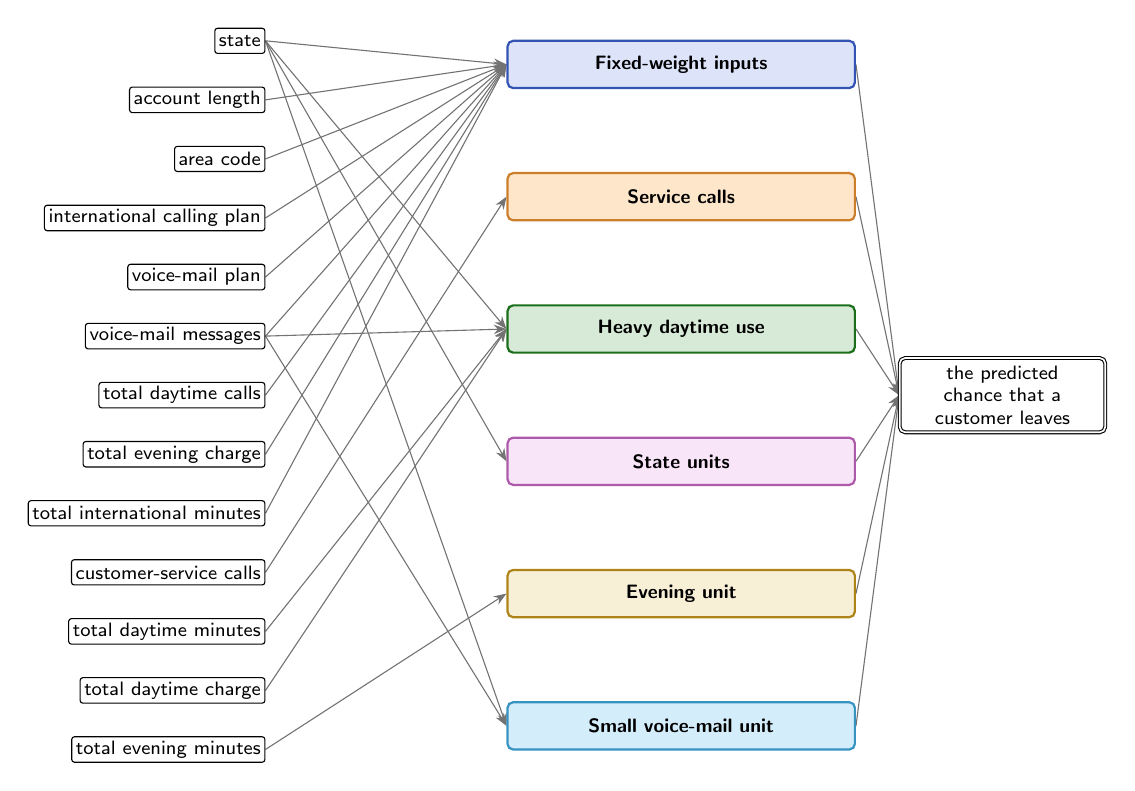
\begin{tikzpicture}[
  font=\sffamily\scriptsize, >={Stealth[length=1.6mm]},
  inp/.style={draw, rounded corners=1pt, fill=white, inner sep=1.5pt, minimum height=3.2mm, anchor=east},
  abox/.style={draw, thick, rounded corners=2pt, align=center, inner sep=3pt, minimum height=6mm, text width=42mm},
  outp/.style={draw, double, rounded corners=2pt, fill=white, align=center, inner sep=3pt, text width=24mm},
  agg/.style={draw=black!55},
]
\node[inp] (i0) at (0,4.5) {state};
\node[inp] (i1) at (0,3.75) {account length};
\node[inp] (i2) at (0,3.0) {area code};
\node[inp] (i3) at (0,2.25) {international calling plan};
\node[inp] (i4) at (0,1.5) {voice-mail plan};
\node[inp] (i5) at (0,0.75) {voice-mail messages};
\node[inp] (i6) at (0,-0.0) {total daytime calls};
\node[inp] (i7) at (0,-0.75) {total evening charge};
\node[inp] (i8) at (0,-1.5) {total international minutes};
\node[inp] (i9) at (0,-2.25) {customer-service calls};
\node[inp] (i10) at (0,-3.0) {total daytime minutes};
\node[inp] (i11) at (0,-3.75) {total daytime charge};
\node[inp] (i12) at (0,-4.5) {total evening minutes};
\node[abox, fill=RoyalBlue!18, draw=RoyalBlue!80!black] (b0) at (5.28,4.2) {\textbf{Fixed-weight inputs}};
\node[abox, fill=BurntOrange!18, draw=BurntOrange!80!black] (b1) at (5.28,2.52) {\textbf{Service calls}};
\node[abox, fill=ForestGreen!18, draw=ForestGreen!80!black] (b2) at (5.28,0.84) {\textbf{Heavy daytime use}};
\node[abox, fill=Orchid!18, draw=Orchid!80!black] (b3) at (5.28,-0.84) {\textbf{State units}};
\node[abox, fill=Goldenrod!18, draw=Goldenrod!80!black] (b4) at (5.28,-2.52) {\textbf{Evening unit}};
\node[abox, fill=Cerulean!18, draw=Cerulean!80!black] (b5) at (5.28,-4.2) {\textbf{Small voice-mail unit}};
\node[outp] (out) at (9.36,0) {the predicted chance that a customer leaves};
\begin{scope}[on background layer]
\draw[->, agg, thin] (i0.east) -- (b0.west);
\draw[->, agg, thin] (i1.east) -- (b0.west);
\draw[->, agg, thin] (i2.east) -- (b0.west);
\draw[->, agg, thin] (i3.east) -- (b0.west);
\draw[->, agg, thin] (i4.east) -- (b0.west);
\draw[->, agg, thin] (i5.east) -- (b0.west);
\draw[->, agg, thin] (i6.east) -- (b0.west);
\draw[->, agg, thin] (i7.east) -- (b0.west);
\draw[->, agg, thin] (i8.east) -- (b0.west);
\draw[->, agg] (b0.east) -- (out.west);
\draw[->, agg, thin] (i9.east) -- (b1.west);
\draw[->, agg] (b1.east) -- (out.west);
\draw[->, agg, thin] (i0.east) -- (b2.west);
\draw[->, agg, thin] (i5.east) -- (b2.west);
\draw[->, agg, thin] (i10.east) -- (b2.west);
\draw[->, agg, thin] (i11.east) -- (b2.west);
\draw[->, agg] (b2.east) -- (out.west);
\draw[->, agg, thin] (i0.east) -- (b3.west);
\draw[->, agg] (b3.east) -- (out.west);
\draw[->, agg, thin] (i12.east) -- (b4.west);
\draw[->, agg] (b4.east) -- (out.west);
\draw[->, agg, thin] (i0.east) -- (b5.west);
\draw[->, agg, thin] (i5.east) -- (b5.west);
\draw[->, agg] (b5.east) -- (out.west);
\end{scope}
\end{tikzpicture}}}%
\caption{The whole model: what feeds it, one level down.}
\label{fig:churn100s4c2:parts-ann87}
\end{figure}
\begin{figure}[H]\centering
\resizebox{\ifdim\width>\linewidth\linewidth\else\width\fi}{!}{%
\definecolor{netup}{HTML}{D95F02}\definecolor{netdown}{HTML}{1B9E77}\definecolor{netmixed}{HTML}{7F7F7F}%
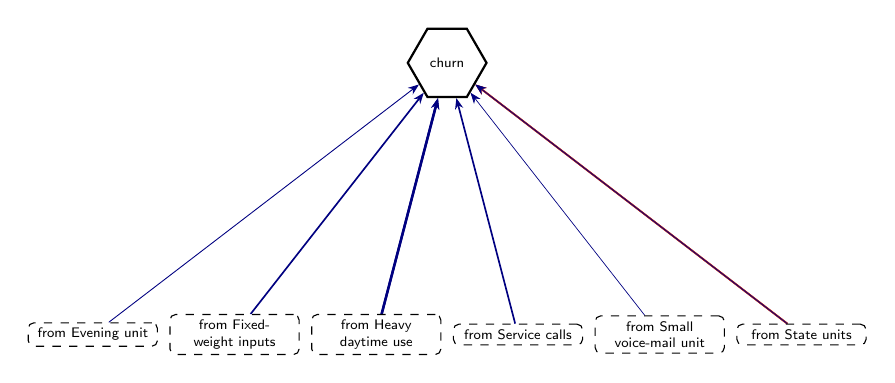
\begin{tikzpicture}[
  font=\sffamily\scriptsize, >={Stealth[length=1.4mm]},
  inp/.style={draw, circle, fill=white, minimum size=3.2mm, inner sep=0pt},
  hid/.style={draw, circle, fill=white, minimum size=5.2mm, inner sep=0.5pt, font=\sffamily\tiny},
  exitbox/.style={draw, thick, rectangle, fill=white, align=center, text width=17mm, minimum height=5mm, inner sep=1.5pt, font=\sffamily\tiny},
  sumbox/.style={draw, thick, dashed, rectangle, fill=white, align=center, text width=17mm, minimum height=5mm, inner sep=1.5pt, font=\sffamily\tiny},
  outp/.style={draw, thick, regular polygon, regular polygon sides=6, fill=white, minimum size=10mm, inner sep=0pt, font=\sffamily\tiny, align=center},
  stub/.style={draw, dashed, rounded corners=2pt, fill=white, align=center, inner sep=2pt, font=\sffamily\tiny, text width=15mm},
  inlab/.style={font=\sffamily\tiny, align=center, text width=15mm, inner sep=1pt, fill=white, fill opacity=0.8, text opacity=1},
  wpos/.style={draw=NavyBlue}, wneg/.style={draw=BrickRed}, wagg/.style={draw=black!45, line width=1.2pt},
  wmix/.style={draw=Plum},
]
\node[outp] (n0) at (5.4,3.45) {churn};
\node[stub] (nfromxxStatexunits) at (9.9,0.0) {from State units};
\node[stub] (nfromxxHeavyxdaytimexuse) at (4.5,0.0) {from Heavy daytime use};
\node[stub] (nfromxxSmallxvoicemmailxunit) at (8.1,0.0) {from Small voice-mail unit};
\node[stub] (nfromxxEveningxunit) at (0.9,0.0) {from Evening unit};
\node[stub] (nfromxxFixedmweightxinputs) at (2.7,0.0) {from Fixed-weight inputs};
\node[stub] (nfromxxServicexcalls) at (6.3,0.0) {from Service calls};
\begin{scope}[on background layer]
\draw[->, wneg, line width=0.60pt] (nfromxxStatexunits) -- (n0);
\draw[->, wpos, line width=0.79pt] (nfromxxHeavyxdaytimexuse) -- (n0);
\draw[->, wpos, line width=0.25pt] (nfromxxSmallxvoicemmailxunit) -- (n0);
\draw[->, wneg, line width=0.67pt] (nfromxxStatexunits) -- (n0);
\draw[->, wpos, line width=0.26pt] (nfromxxStatexunits) -- (n0);
\draw[->, wpos, line width=0.92pt] (nfromxxHeavyxdaytimexuse) -- (n0);
\draw[->, wpos, line width=0.32pt] (nfromxxEveningxunit) -- (n0);
\draw[->, wpos, line width=0.60pt] (nfromxxFixedmweightxinputs) -- (n0);
\draw[->, wpos, line width=0.60pt] (nfromxxServicexcalls) -- (n0);
\end{scope}
\end{tikzpicture}}%
\caption{The whole model: its units and every connection into them. Blue: positive weight (raises the score); red: negative weight (lowers it); thicker: larger weight. Orange outline and up arrow: raises the final prediction; teal and down arrow: lowers it; grey and double arrow: depends.}
\label{fig:churn100s4c2:units-ann87}
\end{figure}
\paragraph{Hypothesis.} The model adds up six parts into one score: fixed-weight inputs, service calls, heavy daytime use, state units, an evening unit and a small voice-mail unit.\,{\scriptsize\textcolor{NavyBlue}{[C046]}}
\paragraph{Evidence.} It is made up of these six parts (each explained below); the score is their sum, which was checked on all 4000 training customers.\,{\scriptsize\textcolor{NavyBlue}{[C046]}} Changing one input at a time across the whole model, an international plan takes a typical customer's chance of leaving from about 3\% to about 31\%, and a voice-mail plan lowers it to under 1\%.\,{\scriptsize\textcolor{NavyBlue}{[C001, C006]}} More daytime minutes raise it in an uneven way, from about 3\% at 112 minutes to about 8\% at 249 minutes, flattening out near the bottom because the predicted chance cannot go much lower.\,{\scriptsize\textcolor{NavyBlue}{[C004]}} In Washington the chance is about 11\%, against about 3\% in West Virginia.\,{\scriptsize\textcolor{NavyBlue}{[C002]}} The model ignores evening calls, international calls, the international charge, night-time calls, the night-time charge and night-time minutes.\,{\scriptsize\textcolor{NavyBlue}{[C040, C041, C042, C043, C044, C045]}}
\par\noindent{\small Evidence plots: Figure~\ref{fig:churn100s4c2:plot-ann87-0}, Figure~\ref{fig:churn100s4c2:plot-ann87-1}.\par}
\begin{figure}[H]\centering
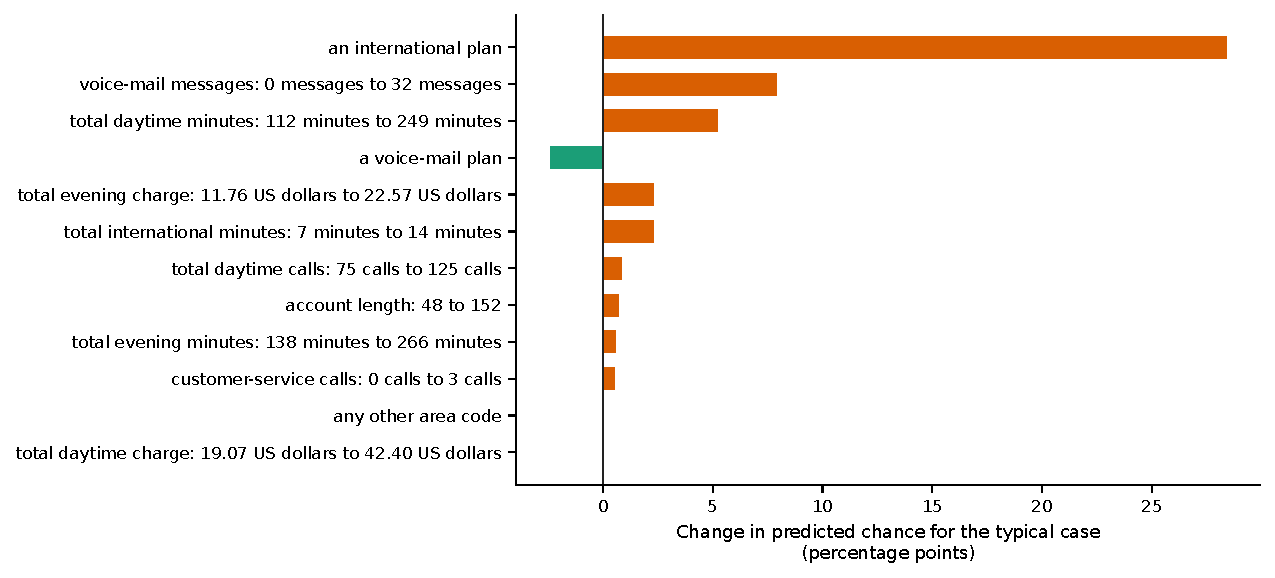
\includegraphics[width=\linewidth,height=0.88\textheight,keepaspectratio]{figures/churn100-s4-c2/ann_87-effects.pdf}
\caption{The whole model: Each input's change in the predicted value for the typical case across the whole model, largest first (orange: raises it, teal: lowers it).}
\label{fig:churn100s4c2:plot-ann87-0}
\end{figure}
\begin{figure}[H]\centering
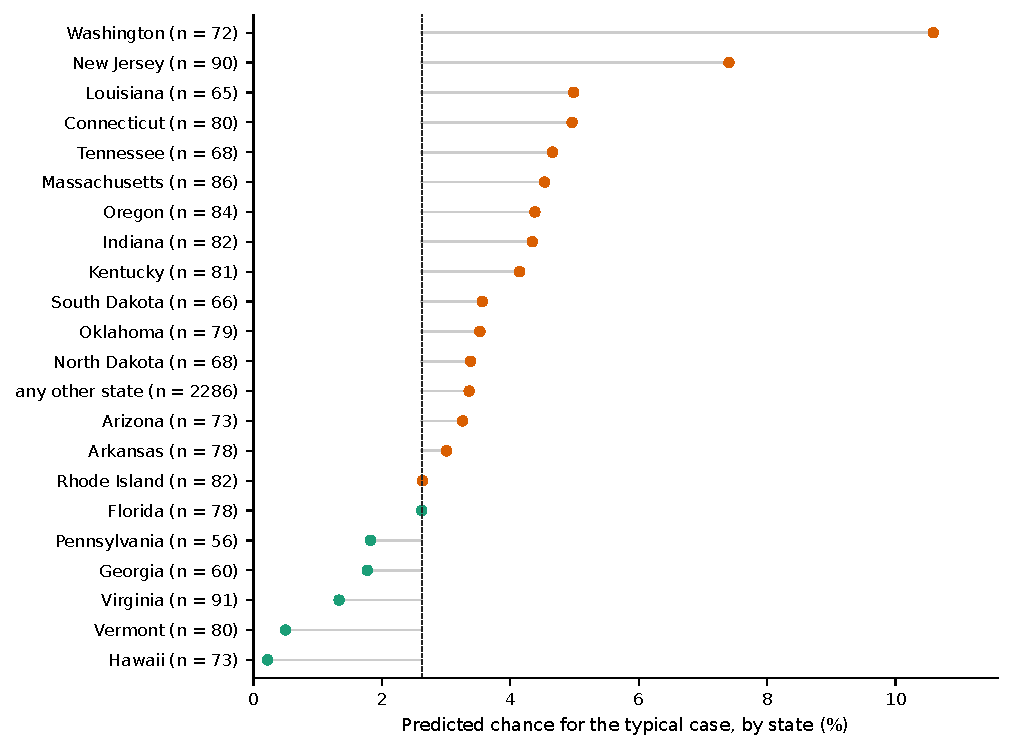
\includegraphics[width=\linewidth,height=0.88\textheight,keepaspectratio]{figures/churn100-s4-c2/ann_87-levels-state.pdf}
\caption{The whole model: Every level of state the model reads: the predicted value for the typical case at that level (dashed: the reference level); n = training customers; grey: few customers or not supported.}
\label{fig:churn100s4c2:plot-ann87-1}
\end{figure}
\par\smallskip\noindent{\small \textbf{Dive deeper:} Fixed-weight inputs (\ref{rd:ann79}); Service calls (\ref{rd:ann86}); Heavy daytime use (\ref{rd:ann82}); State units (\ref{rd:ann85}); Evening unit (\ref{rd:ann83}); Small voice-mail unit (\ref{rd:ann84}). Technical detail: \ref{tech:ann87}.\par}
\subsubsection{Fixed-weight inputs}\label{rd:ann79}
\noindent{\footnotesize Part of: The whole model (\ref{rd:ann87}).\par}
\noindent{\small Figure~\ref{fig:churn100s4c2:parts-ann79} shows what feeds this part; Figure~\ref{fig:churn100s4c2:units-ann79} its units and every connection into them (dashed boxes: connections from or to other parts, drawn in their own sections).\par}
\begin{figure}[H]\centering
\resizebox{!}{\ifdim\height>0.5\textheight 0.5\textheight\else\height\fi}{%
\resizebox{\ifdim\width>\linewidth\linewidth\else\width\fi}{!}{%
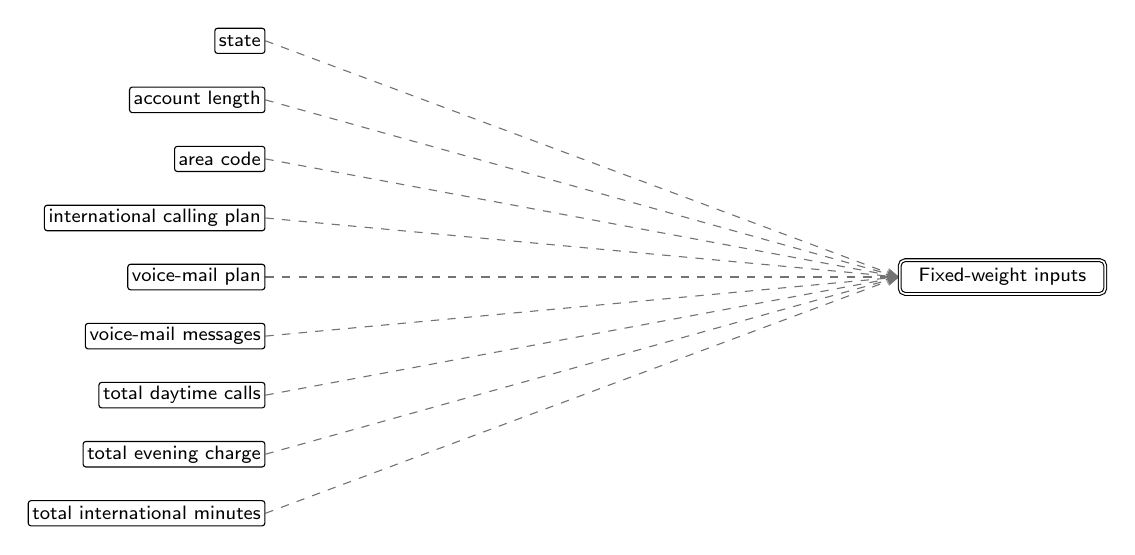
\begin{tikzpicture}[
  font=\sffamily\scriptsize, >={Stealth[length=1.6mm]},
  inp/.style={draw, rounded corners=1pt, fill=white, inner sep=1.5pt, minimum height=3.2mm, anchor=east},
  abox/.style={draw, thick, rounded corners=2pt, align=center, inner sep=3pt, minimum height=6mm, text width=42mm},
  outp/.style={draw, double, rounded corners=2pt, fill=white, align=center, inner sep=3pt, text width=24mm},
  agg/.style={draw=black!55},
]
\node[inp] (i0) at (0,3.0) {state};
\node[inp] (i1) at (0,2.25) {account length};
\node[inp] (i2) at (0,1.5) {area code};
\node[inp] (i3) at (0,0.75) {international calling plan};
\node[inp] (i4) at (0,-0.0) {voice-mail plan};
\node[inp] (i5) at (0,-0.75) {voice-mail messages};
\node[inp] (i6) at (0,-1.5) {total daytime calls};
\node[inp] (i7) at (0,-2.25) {total evening charge};
\node[inp] (i8) at (0,-3.0) {total international minutes};
\node[outp] (out) at (9.36,0) {Fixed-weight inputs};
\begin{scope}[on background layer]
\draw[->, agg, thin, dashed] (i0.east) -- (out.west);
\draw[->, agg, thin, dashed] (i1.east) -- (out.west);
\draw[->, agg, thin, dashed] (i2.east) -- (out.west);
\draw[->, agg, thin, dashed] (i3.east) -- (out.west);
\draw[->, agg, thin, dashed] (i4.east) -- (out.west);
\draw[->, agg, thin, dashed] (i5.east) -- (out.west);
\draw[->, agg, thin, dashed] (i6.east) -- (out.west);
\draw[->, agg, thin, dashed] (i7.east) -- (out.west);
\draw[->, agg, thin, dashed] (i8.east) -- (out.west);
\end{scope}
\end{tikzpicture}}}%
\caption{Fixed-weight inputs: what feeds it, one level down.}
\label{fig:churn100s4c2:parts-ann79}
\end{figure}
\begin{figure}[H]\centering
\resizebox{\ifdim\width>\linewidth\linewidth\else\width\fi}{!}{%
\definecolor{netup}{HTML}{D95F02}\definecolor{netdown}{HTML}{1B9E77}\definecolor{netmixed}{HTML}{7F7F7F}%
\begin{tikzpicture}[
  font=\sffamily\scriptsize, >={Stealth[length=1.4mm]},
  inp/.style={draw, circle, fill=white, minimum size=3.2mm, inner sep=0pt},
  hid/.style={draw, circle, fill=white, minimum size=5.2mm, inner sep=0.5pt, font=\sffamily\tiny},
  exitbox/.style={draw, thick, rectangle, fill=white, align=center, text width=17mm, minimum height=5mm, inner sep=1.5pt, font=\sffamily\tiny},
  sumbox/.style={draw, thick, dashed, rectangle, fill=white, align=center, text width=17mm, minimum height=5mm, inner sep=1.5pt, font=\sffamily\tiny},
  outp/.style={draw, thick, regular polygon, regular polygon sides=6, fill=white, minimum size=10mm, inner sep=0pt, font=\sffamily\tiny, align=center},
  stub/.style={draw, dashed, rounded corners=2pt, fill=white, align=center, inner sep=2pt, font=\sffamily\tiny, text width=15mm},
  inlab/.style={font=\sffamily\tiny, align=center, text width=15mm, inner sep=1pt, fill=white, fill opacity=0.8, text opacity=1},
  wpos/.style={draw=NavyBlue}, wneg/.style={draw=BrickRed}, wagg/.style={draw=black!45, line width=1.2pt},
  wmix/.style={draw=Plum},
]
\node[exitbox] (nidentityxlin) at (5.85,1.9) {Fixed-weight inputs $\uparrow$};
\node[inp, draw=netmixed, very thick] (ngrpxxstate) at (4.5,0.0) {};
\path (ngrpxxstate.south) node[inlab, anchor=north] (labngrpxxstate) {state (22 of 51 used) $\updownarrow$};
\node[inp, draw=netup, very thick] (ninxxaccountxlength) at (1.8,-1.05) {};
\path (ninxxaccountxlength.south) node[inlab, anchor=north] (labninxxaccountxlength) {account length $\uparrow$};
\node[inp, draw=netup, very thick] (ninxxareaxcodex415) at (3.6,-1.05) {};
\path (ninxxareaxcodex415.south) node[inlab, anchor=north] (labninxxareaxcodex415) {area code 415 $\uparrow$};
\node[inp, draw=netup, very thick] (ninxxinternationalxplan) at (2.7,0.0) {};
\path (ninxxinternationalxplan.south) node[inlab, anchor=north] (labninxxinternationalxplan) {an international plan $\uparrow$};
\node[inp, draw=netdown, very thick] (ninxxvoicexmailxplan) at (0.9,0.0) {};
\path (ninxxvoicexmailxplan.south) node[inlab, anchor=north] (labninxxvoicexmailxplan) {a voice-mail plan $\downarrow$};
\node[inp, draw=netup, very thick] (ninxxtotalxdayxcalls) at (5.4,-1.05) {};
\path (ninxxtotalxdayxcalls.south) node[inlab, anchor=north] (labninxxtotalxdayxcalls) {total daytime calls $\uparrow$};
\node[inp, draw=netup, very thick] (ninxxtotalxevexcharge) at (6.3,0.0) {};
\path (ninxxtotalxevexcharge.south) node[inlab, anchor=north] (labninxxtotalxevexcharge) {total evening charge $\uparrow$};
\node[inp, draw=netup, very thick] (ninxxtotalxintlxminutes) at (8.1,0.0) {};
\path (ninxxtotalxintlxminutes.south) node[inlab, anchor=north] (labninxxtotalxintlxminutes) {total international minutes $\uparrow$};
\node[inp, draw=netup, very thick] (ninxxnumberxvmailxmessages) at (9.9,0.0) {};
\path (ninxxnumberxvmailxmessages.south) node[inlab, anchor=north] (labninxxnumberxvmailxmessages) {voice-mail messages $\uparrow$};
\node[stub] (ntoxxthexmodelxoutput) at (5.4,3.45) {to the model output};
\begin{scope}[on background layer]
\node[fit=(nidentityxlin) , inner sep=8pt, rounded corners=5pt, fill=BurntOrange!10, draw=BurntOrange!45] (clu0) {};
\draw[->, wpos, line width=0.29pt] (ninxxaccountxlength) -- (nidentityxlin);
\draw[->, wpos, line width=0.25pt] (ninxxareaxcodex415) -- (nidentityxlin);
\draw[->, wpos, line width=0.54pt] (ninxxinternationalxplan) -- (nidentityxlin);
\draw[->, wneg, line width=0.64pt] (ninxxvoicexmailxplan) -- (nidentityxlin);
\draw[->, wpos, line width=0.30pt] (ninxxtotalxdayxcalls) -- (nidentityxlin);
\draw[->, wpos, line width=0.37pt] (ninxxtotalxevexcharge) -- (nidentityxlin);
\draw[->, wpos, line width=0.37pt] (ninxxtotalxintlxminutes) -- (nidentityxlin);
\draw[->, wpos, line width=0.47pt] (ninxxnumberxvmailxmessages) -- (nidentityxlin);
\draw[->, wpos, line width=0.60pt] (nidentityxlin) -- (ntoxxthexmodelxoutput);
\draw[->, wmix, line width=0.38pt] (ngrpxxstate) -- node[pos=0.8, sloped, above, font=\sffamily\tiny, inner sep=1pt, fill=white, fill opacity=0.8, text opacity=1] {21 edges, -0.37 to +0.16} (nidentityxlin);
\end{scope}
\node[font=\sffamily\scriptsize\bfseries, text=BurntOrange!55!black, anchor=south west, inner sep=1pt, fill=white, fill opacity=0.85, text opacity=1] at (clu0.north west) {Fixed-weight inputs};
\end{tikzpicture}}%
\caption{Fixed-weight inputs: its units and every connection into them. Blue: positive weight (raises the score); red: negative weight (lowers it); thicker: larger weight. Orange outline and up arrow: raises the final prediction; teal and down arrow: lowers it; grey and double arrow: depends.}
\label{fig:churn100s4c2:units-ann79}
\end{figure}
\paragraph{Hypothesis.} This part adds up most inputs with fixed weights: an international plan, voice-mail messages, the evening charge and international minutes raise the chance of leaving, steadily for the numbers, and a voice-mail plan lowers it.\,{\scriptsize\textcolor{NavyBlue}{[C047, C049, C055, C056, C051]}}
\paragraph{Evidence.} Through it, an international plan takes a typical customer from about 3\% to about 31\%, and a voice-mail plan lowers the chance to under 1\%.\,{\scriptsize\textcolor{NavyBlue}{[C047, C051]}} More voice-mail messages raise it steadily, from about 3\% at 0 to about 10\% at 32 messages, flattening out near the bottom because the predicted chance cannot go much lower.\,{\scriptsize\textcolor{NavyBlue}{[C049]}} Through it, the state moves the chance from about 3\% in West Virginia to about 11\% in Washington and about 7\% in New Jersey, and to under 1\% in Hawaii and in Rhode Island (72 to 122 training customers per state).\,{\scriptsize\textcolor{NavyBlue}{[C048, C050, C052, C053]}} Its formula reproduces the part exactly on all 4000 training customers.\,{\scriptsize\textcolor{NavyBlue}{[C076]}}
\par\noindent{\small Evidence plots: Figure~\ref{fig:churn100s4c2:plot-ann79-0}, Figure~\ref{fig:churn100s4c2:plot-ann79-1}, Figure~\ref{fig:churn100s4c2:plot-ann79-2}, Figure~\ref{fig:churn100s4c2:plot-ann79-3}.\par}
\begin{figure}[H]\centering
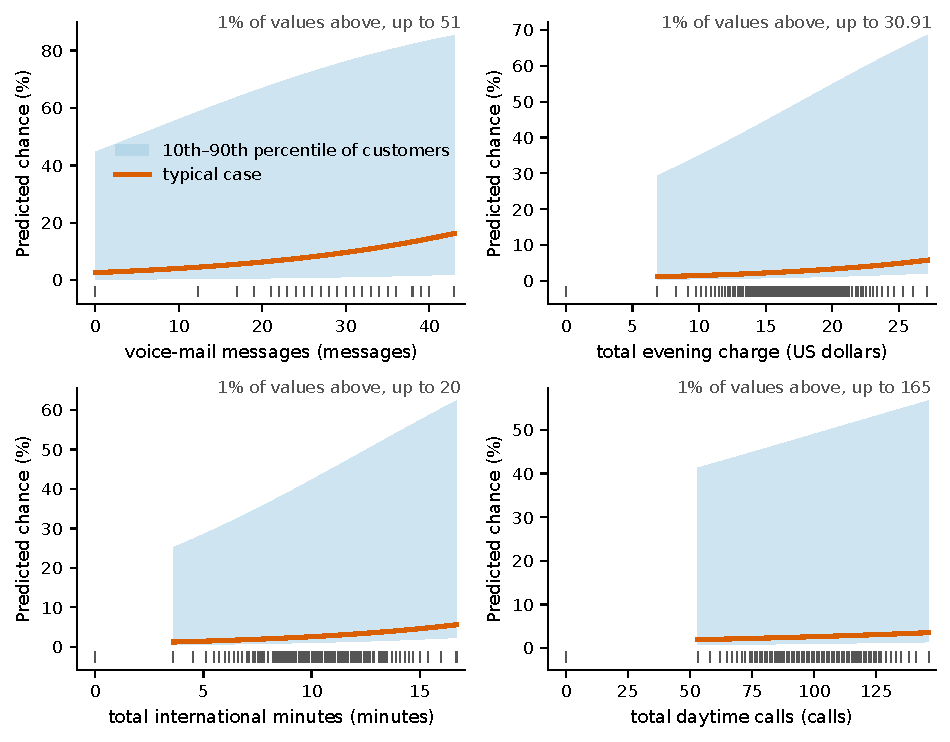
\includegraphics[width=\linewidth,height=0.88\textheight,keepaspectratio]{figures/churn100-s4-c2/ann_79-response.pdf}
\caption{Fixed-weight inputs: Response curves through this part: the typical case (bold), the 10th to 90th percentile of individual customers (band), the fold or step point (dashed) with its spread across them (grey), and the observed values (ticks).}
\label{fig:churn100s4c2:plot-ann79-0}
\end{figure}
\begin{figure}[H]\centering
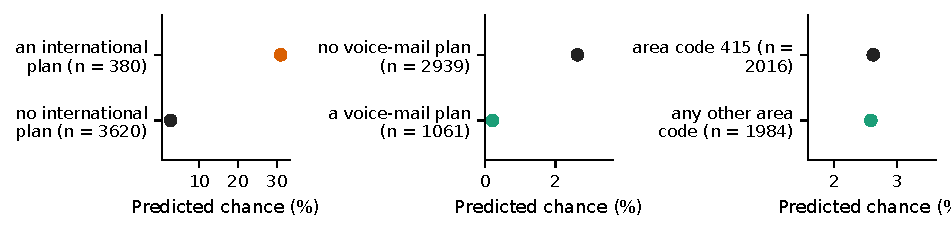
\includegraphics[width=\linewidth,height=0.88\textheight,keepaspectratio]{figures/churn100-s4-c2/ann_79-categories-small.pdf}
\caption{Fixed-weight inputs: The predicted value for the typical case at each level, through this part (n = training customers; grey: fewer than 20).}
\label{fig:churn100s4c2:plot-ann79-1}
\end{figure}
\begin{figure}[H]\centering
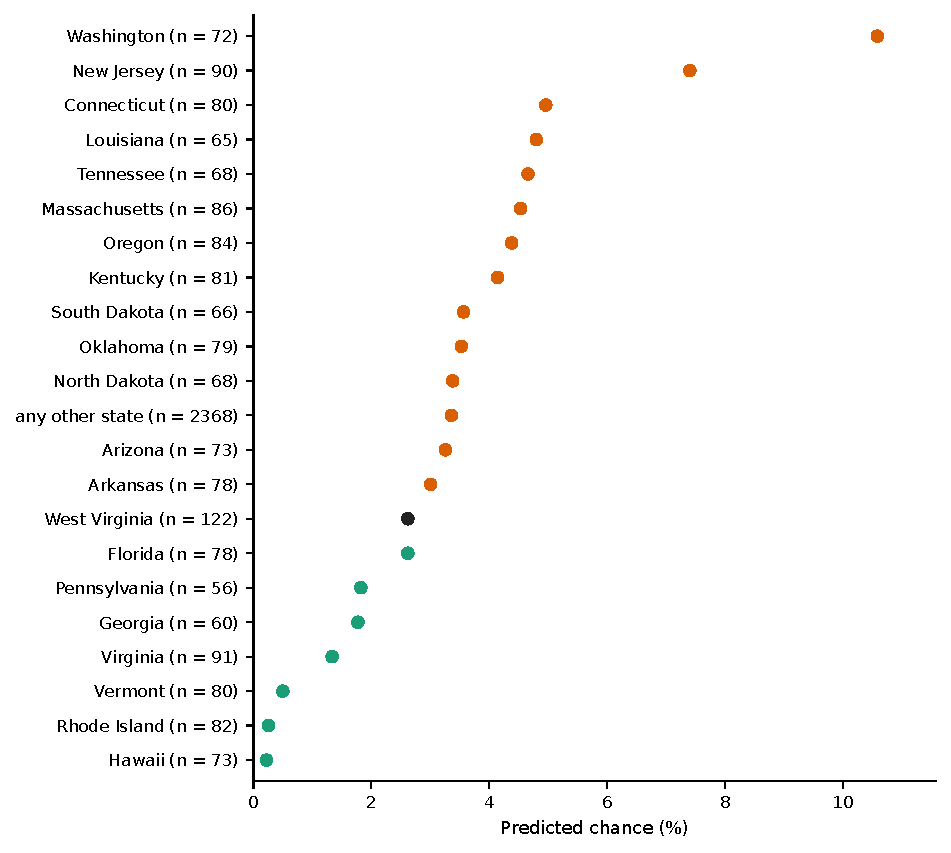
\includegraphics[width=\linewidth,height=0.88\textheight,keepaspectratio]{figures/churn100-s4-c2/ann_79-categories-C048.pdf}
\caption{Fixed-weight inputs: The predicted value for the typical case at each level, through this part (n = training customers; grey: fewer than 20).}
\label{fig:churn100s4c2:plot-ann79-2}
\end{figure}
\begin{figure}[H]\centering
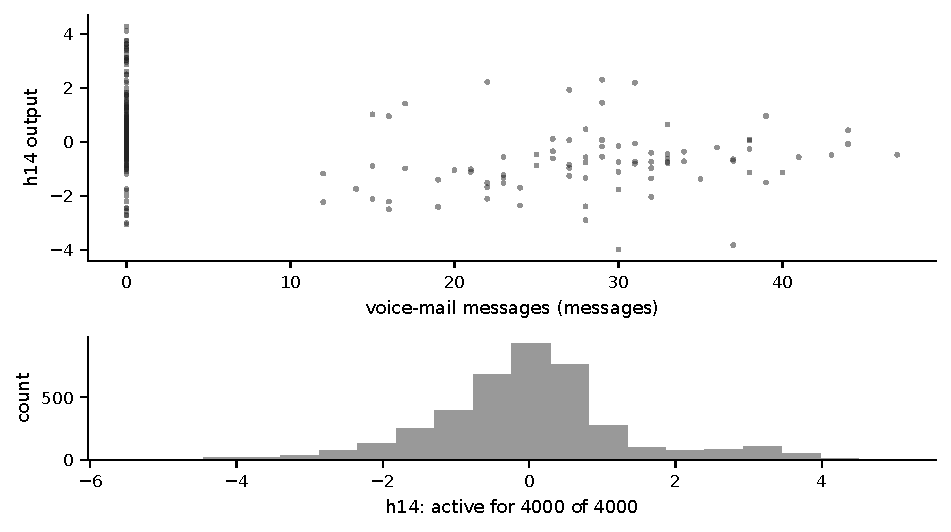
\includegraphics[width=\linewidth,height=0.88\textheight,keepaspectratio]{figures/churn100-s4-c2/ann_79-units.pdf}
\caption{Fixed-weight inputs: This part's hidden units: each unit's output against its main numeric input (top) and how often it is active (bottom).}
\label{fig:churn100s4c2:plot-ann79-3}
\end{figure}
\par\smallskip\noindent{\small Technical detail: \ref{tech:ann79}.\par}
\subsubsection{Service calls}\label{rd:ann86}
\noindent{\footnotesize Part of: The whole model (\ref{rd:ann87}).\par}
\noindent{\small Figure~\ref{fig:churn100s4c2:parts-ann86} shows what feeds this part; Figure~\ref{fig:churn100s4c2:units-ann86} its units and every connection into them (dashed boxes: connections from or to other parts, drawn in their own sections).\par}
\begin{figure}[H]\centering
\resizebox{!}{\ifdim\height>0.5\textheight 0.5\textheight\else\height\fi}{%
\resizebox{\ifdim\width>\linewidth\linewidth\else\width\fi}{!}{%
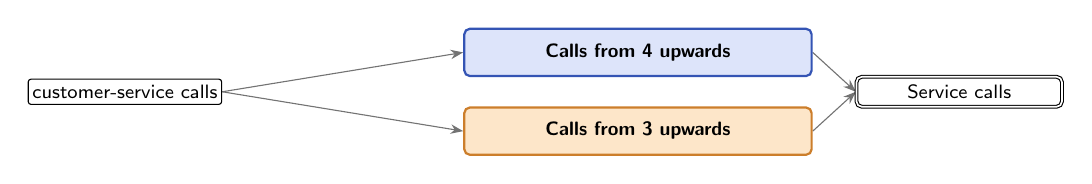
\begin{tikzpicture}[
  font=\sffamily\scriptsize, >={Stealth[length=1.6mm]},
  inp/.style={draw, rounded corners=1pt, fill=white, inner sep=1.5pt, minimum height=3.2mm, anchor=east},
  abox/.style={draw, thick, rounded corners=2pt, align=center, inner sep=3pt, minimum height=6mm, text width=42mm},
  outp/.style={draw, double, rounded corners=2pt, fill=white, align=center, inner sep=3pt, text width=24mm},
  agg/.style={draw=black!55},
]
\node[inp] (i0) at (0,-0.0) {customer-service calls};
\node[abox, fill=RoyalBlue!18, draw=RoyalBlue!80!black] (b0) at (5.28,0.5) {\textbf{Calls from 4 upwards}};
\node[abox, fill=BurntOrange!18, draw=BurntOrange!80!black] (b1) at (5.28,-0.5) {\textbf{Calls from 3 upwards}};
\node[outp] (out) at (9.36,0) {Service calls};
\begin{scope}[on background layer]
\draw[->, agg, thin] (i0.east) -- (b0.west);
\draw[->, agg] (b0.east) -- (out.west);
\draw[->, agg, thin] (i0.east) -- (b1.west);
\draw[->, agg] (b1.east) -- (out.west);
\end{scope}
\end{tikzpicture}}}%
\caption{Service calls: what feeds it, one level down.}
\label{fig:churn100s4c2:parts-ann86}
\end{figure}
\begin{figure}[H]\centering
\resizebox{\ifdim\width>\linewidth\linewidth\else\width\fi}{!}{%
\definecolor{netup}{HTML}{D95F02}\definecolor{netdown}{HTML}{1B9E77}\definecolor{netmixed}{HTML}{7F7F7F}%
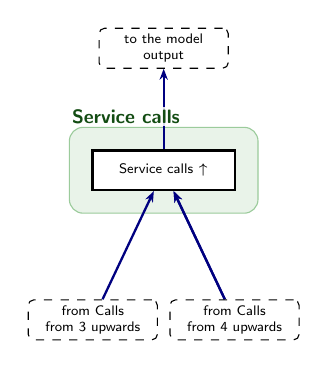
\begin{tikzpicture}[
  font=\sffamily\scriptsize, >={Stealth[length=1.4mm]},
  inp/.style={draw, circle, fill=white, minimum size=3.2mm, inner sep=0pt},
  hid/.style={draw, circle, fill=white, minimum size=5.2mm, inner sep=0.5pt, font=\sffamily\tiny},
  exitbox/.style={draw, thick, rectangle, fill=white, align=center, text width=17mm, minimum height=5mm, inner sep=1.5pt, font=\sffamily\tiny},
  sumbox/.style={draw, thick, dashed, rectangle, fill=white, align=center, text width=17mm, minimum height=5mm, inner sep=1.5pt, font=\sffamily\tiny},
  outp/.style={draw, thick, regular polygon, regular polygon sides=6, fill=white, minimum size=10mm, inner sep=0pt, font=\sffamily\tiny, align=center},
  stub/.style={draw, dashed, rounded corners=2pt, fill=white, align=center, inner sep=2pt, font=\sffamily\tiny, text width=15mm},
  inlab/.style={font=\sffamily\tiny, align=center, text width=15mm, inner sep=1pt, fill=white, fill opacity=0.8, text opacity=1},
  wpos/.style={draw=NavyBlue}, wneg/.style={draw=BrickRed}, wagg/.style={draw=black!45, line width=1.2pt},
  wmix/.style={draw=Plum},
]
\node[exitbox] (nidentityxsvc) at (1.8,1.9) {Service calls $\uparrow$};
\node[stub] (nfromxxCallsxfromx3xupwards) at (0.9,0.0) {from Calls from 3 upwards};
\node[stub] (nfromxxCallsxfromx4xupwards) at (2.7,0.0) {from Calls from 4 upwards};
\node[stub] (ntoxxthexmodelxoutput) at (1.8,3.45) {to the model output};
\begin{scope}[on background layer]
\node[fit=(nidentityxsvc) , inner sep=8pt, rounded corners=5pt, fill=ForestGreen!10, draw=ForestGreen!45] (clu0) {};
\draw[->, wpos, line width=0.83pt] (nfromxxCallsxfromx3xupwards) -- (nidentityxsvc);
\draw[->, wpos, line width=0.87pt] (nfromxxCallsxfromx4xupwards) -- (nidentityxsvc);
\draw[->, wpos, line width=0.79pt] (nfromxxCallsxfromx4xupwards) -- (nidentityxsvc);
\draw[->, wpos, line width=0.60pt] (nidentityxsvc) -- (ntoxxthexmodelxoutput);
\end{scope}
\node[font=\sffamily\scriptsize\bfseries, text=ForestGreen!55!black, anchor=south west, inner sep=1pt, fill=white, fill opacity=0.85, text opacity=1] at (clu0.north west) {Service calls};
\end{tikzpicture}}%
\caption{Service calls: its units and every connection into them. Blue: positive weight (raises the score); red: negative weight (lowers it); thicker: larger weight. Orange outline and up arrow: raises the final prediction; teal and down arrow: lowers it; grey and double arrow: depends.}
\label{fig:churn100s4c2:units-ann86}
\end{figure}
\paragraph{Hypothesis.} This part raises the chance of leaving with calls to customer service from 3 calls upwards, slowly at first, then faster; it adds up two parts.\,{\scriptsize\textcolor{NavyBlue}{[C079, C078, C077]}}
\paragraph{Evidence.} It is made of two parts that are added: calls from 3 upwards and calls from 4 upwards.\,{\scriptsize\textcolor{NavyBlue}{[C079]}} From 3 calls upwards it adds to the chance slowly at first, then faster: for a typical such customer, 4 calls take it from about 3\% to about 18\%.\,{\scriptsize\textcolor{NavyBlue}{[C078]}} Up to 3 calls it barely moves a typical customer's chance, which stays at about 3\%, rising slowly at first, then faster.\,{\scriptsize\textcolor{NavyBlue}{[C077]}}
\par\noindent{\small Evidence plots: Figure~\ref{fig:churn100s4c2:plot-ann86-0}, Figure~\ref{fig:churn100s4c2:plot-ann86-1}, Figure~\ref{fig:churn100s4c2:plot-ann86-2}.\par}
\par\noindent{\small Figure~\ref{fig:churn100s4c2:plot-ann86-1} shows this part's own output, unit h15: it switches on at about 2.899 calls of customer-service calls, and is zero below.\par}
\begin{figure}[H]\centering
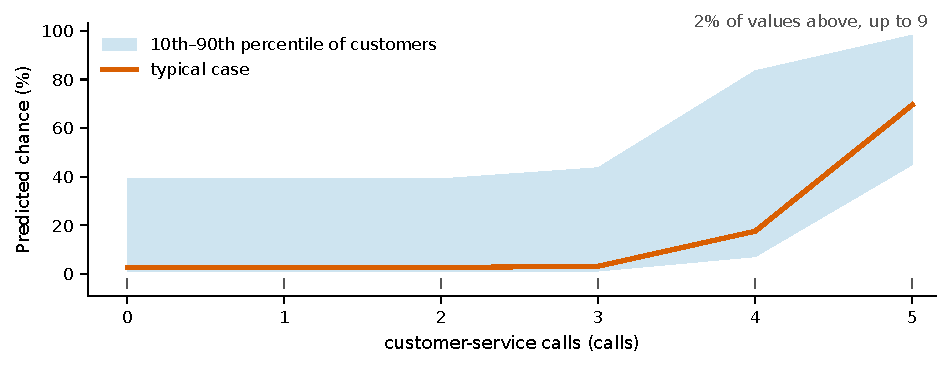
\includegraphics[width=\linewidth,height=0.88\textheight,keepaspectratio]{figures/churn100-s4-c2/ann_86-response.pdf}
\caption{Service calls: Response curves through this part: the typical case (bold), the 10th to 90th percentile of individual customers (band), the fold or step point (dashed) with its spread across them (grey), and the observed values (ticks).}
\label{fig:churn100s4c2:plot-ann86-0}
\end{figure}
\begin{figure}[H]\centering
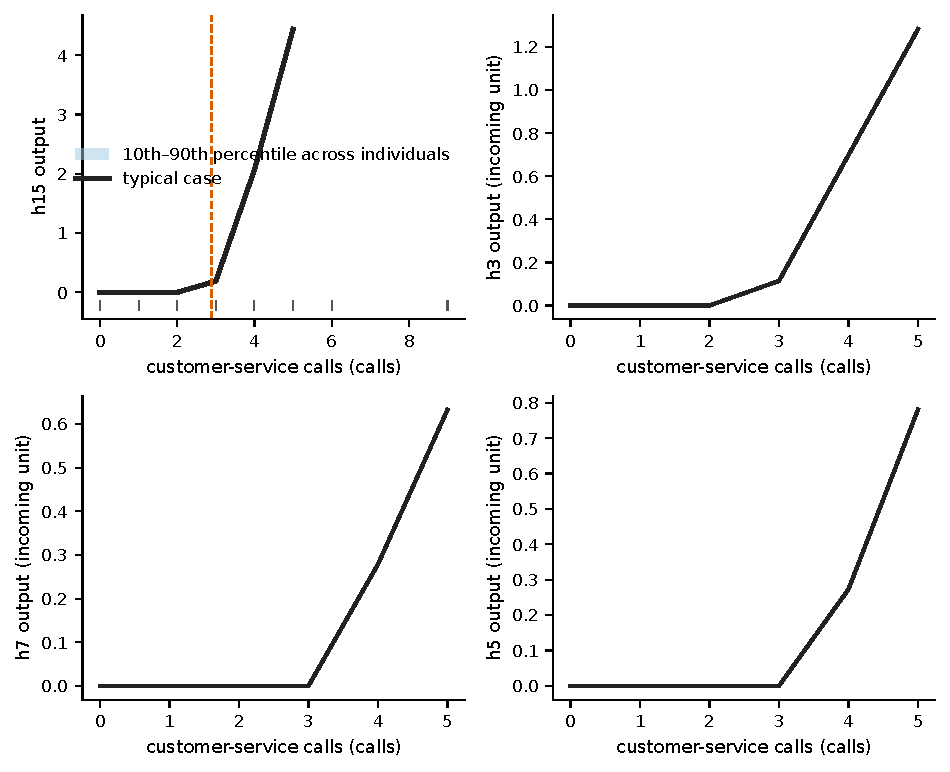
\includegraphics[width=\linewidth,height=0.88\textheight,keepaspectratio]{figures/churn100-s4-c2/ann_86-partial-identity_svc.pdf}
\caption{Service calls: This part's own output, unit h15 (combines 3 non-linear units), on its own scale (its activation), with every other input at the typical case; it is active for 848 of 4000. Bold: the typical case; band: 10th to 90th percentile across individuals; dashed: where it switches on; ticks: the data.}
\label{fig:churn100s4c2:plot-ann86-1}
\end{figure}
\begin{figure}[H]\centering
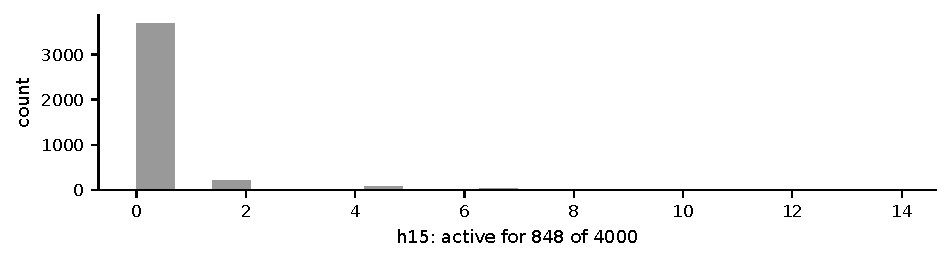
\includegraphics[width=\linewidth,height=0.88\textheight,keepaspectratio]{figures/churn100-s4-c2/ann_86-units.pdf}
\caption{Service calls: This part's hidden units: each unit's output against its main numeric input (top) and how often it is active (bottom).}
\label{fig:churn100s4c2:plot-ann86-2}
\end{figure}
\par\smallskip\noindent{\small \textbf{Dive deeper:} Calls from 4 upwards (\ref{rd:ann81}); Calls from 3 upwards (\ref{rd:ann80}). Technical detail: \ref{tech:ann86}.\par}
\subsubsection{Calls from 4 upwards}\label{rd:ann81}
\noindent{\footnotesize Part of: Service calls (\ref{rd:ann86}).\par}
\noindent{\small Figure~\ref{fig:churn100s4c2:parts-ann81} shows what feeds this part; Figure~\ref{fig:churn100s4c2:units-ann81} its units and every connection into them (dashed boxes: connections from or to other parts, drawn in their own sections).\par}
\begin{figure}[H]\centering
\resizebox{!}{\ifdim\height>0.5\textheight 0.5\textheight\else\height\fi}{%
\resizebox{\ifdim\width>\linewidth\linewidth\else\width\fi}{!}{%
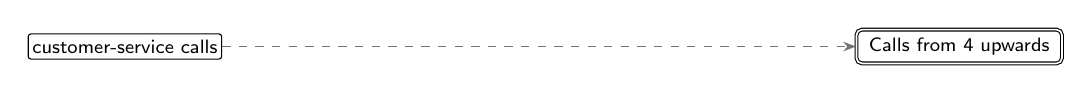
\begin{tikzpicture}[
  font=\sffamily\scriptsize, >={Stealth[length=1.6mm]},
  inp/.style={draw, rounded corners=1pt, fill=white, inner sep=1.5pt, minimum height=3.2mm, anchor=east},
  abox/.style={draw, thick, rounded corners=2pt, align=center, inner sep=3pt, minimum height=6mm, text width=42mm},
  outp/.style={draw, double, rounded corners=2pt, fill=white, align=center, inner sep=3pt, text width=24mm},
  agg/.style={draw=black!55},
]
\node[inp] (i0) at (0,-0.0) {customer-service calls};
\node[outp] (out) at (9.36,0) {Calls from 4 upwards};
\begin{scope}[on background layer]
\draw[->, agg, thin, dashed] (i0.east) -- (out.west);
\end{scope}
\end{tikzpicture}}}%
\caption{Calls from 4 upwards: what feeds it, one level down.}
\label{fig:churn100s4c2:parts-ann81}
\end{figure}
\begin{figure}[H]\centering
\resizebox{\ifdim\width>\linewidth\linewidth\else\width\fi}{!}{%
\definecolor{netup}{HTML}{D95F02}\definecolor{netdown}{HTML}{1B9E77}\definecolor{netmixed}{HTML}{7F7F7F}%
\begin{tikzpicture}[
  font=\sffamily\scriptsize, >={Stealth[length=1.4mm]},
  inp/.style={draw, circle, fill=white, minimum size=3.2mm, inner sep=0pt},
  hid/.style={draw, circle, fill=white, minimum size=5.2mm, inner sep=0.5pt, font=\sffamily\tiny},
  exitbox/.style={draw, thick, rectangle, fill=white, align=center, text width=17mm, minimum height=5mm, inner sep=1.5pt, font=\sffamily\tiny},
  sumbox/.style={draw, thick, dashed, rectangle, fill=white, align=center, text width=17mm, minimum height=5mm, inner sep=1.5pt, font=\sffamily\tiny},
  outp/.style={draw, thick, regular polygon, regular polygon sides=6, fill=white, minimum size=10mm, inner sep=0pt, font=\sffamily\tiny, align=center},
  stub/.style={draw, dashed, rounded corners=2pt, fill=white, align=center, inner sep=2pt, font=\sffamily\tiny, text width=15mm},
  inlab/.style={font=\sffamily\tiny, align=center, text width=15mm, inner sep=1pt, fill=white, fill opacity=0.8, text opacity=1},
  wpos/.style={draw=NavyBlue}, wneg/.style={draw=BrickRed}, wagg/.style={draw=black!45, line width=1.2pt},
  wmix/.style={draw=Plum},
]
\node[hid] (n6713) at (2.0,3.25) {h5};
\node[hid] (n9436) at (2.0,1.9) {h7};
\node[inp, draw=netup, very thick] (ninxxnumberxcustomerxservicexcalls) at (2.0,0.0) {};
\path (ninxxnumberxcustomerxservicexcalls.south) node[inlab, anchor=north] (labninxxnumberxcustomerxservicexcalls) {customer-service calls $\uparrow$};
\node[stub] (ntoxxServicexcalls) at (2.0,4.8) {to Service calls};
\begin{scope}[on background layer]
\node[fit=(n6713) (n9436) , inner sep=8pt, rounded corners=5pt, fill=ForestGreen!10, draw=ForestGreen!45] (clu0) {};
\draw[->, wpos, line width=0.75pt] (n9436) -- (n6713);
\draw[->, wpos, line width=0.41pt] (ninxxnumberxcustomerxservicexcalls) -- (n9436);
\draw[->, wpos, line width=0.87pt] (n9436) -- (ntoxxServicexcalls);
\draw[->, wpos, line width=0.79pt] (n6713) -- (ntoxxServicexcalls);
\end{scope}
\node[font=\sffamily\scriptsize\bfseries, text=ForestGreen!55!black, anchor=south west, inner sep=1pt, fill=white, fill opacity=0.85, text opacity=1] at (clu0.north west) {Calls from 4 upwards};
\end{tikzpicture}}%
\caption{Calls from 4 upwards: its units and every connection into them. Blue: positive weight (raises the score); red: negative weight (lowers it); thicker: larger weight. Orange outline and up arrow: raises the final prediction; teal and down arrow: lowers it; grey and double arrow: depends.}
\label{fig:churn100s4c2:units-ann81}
\end{figure}
\paragraph{Hypothesis.} This part raises the chance of leaving from 4 customer-service calls upwards, slowly at first, then faster.\,{\scriptsize\textcolor{NavyBlue}{[C093]}}
\paragraph{Evidence.} It acts on 318 of 4000 training customers, 159 of whom left; for the typical customer it acts on, the chance is about 8\% without it and about 18\% with it.\,{\scriptsize\textcolor{NavyBlue}{[C094]}} Through it, the chance rises slowly at first, then faster: 4 calls take a typical such customer from about 3\% to about 6\%.\,{\scriptsize\textcolor{NavyBlue}{[C093]}} Its formula reproduces the part exactly on all 4000 training customers.\,{\scriptsize\textcolor{NavyBlue}{[C095]}}
\par\noindent{\small Evidence plots: Figure~\ref{fig:churn100s4c2:plot-ann81-0}, Figure~\ref{fig:churn100s4c2:plot-ann81-1}, Figure~\ref{fig:churn100s4c2:plot-ann81-2}.\par}
\par\noindent{\small Figure~\ref{fig:churn100s4c2:plot-ann81-0} shows this part's own output, unit h7: it switches on at about 3.212 calls of customer-service calls, and is zero below.\par}
\par\noindent{\small Figure~\ref{fig:churn100s4c2:plot-ann81-1} shows this part's own output, unit h5: it switches on at about 3.463 calls of customer-service calls, and is zero below.\par}
\begin{figure}[H]\centering
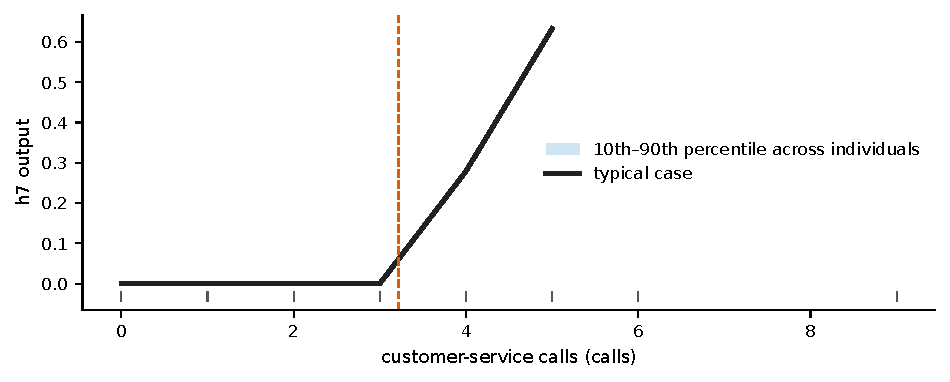
\includegraphics[width=\linewidth,height=0.88\textheight,keepaspectratio]{figures/churn100-s4-c2/ann_81-partial-9436.pdf}
\caption{Calls from 4 upwards: This part's own output, unit h7 (the output of 'Calls from 4 upwards'), on its own scale (its activation), with every other input at the typical case; it is active for 318 of 4000. Bold: the typical case; band: 10th to 90th percentile across individuals; dashed: where it switches on; ticks: the data.}
\label{fig:churn100s4c2:plot-ann81-0}
\end{figure}
\begin{figure}[H]\centering
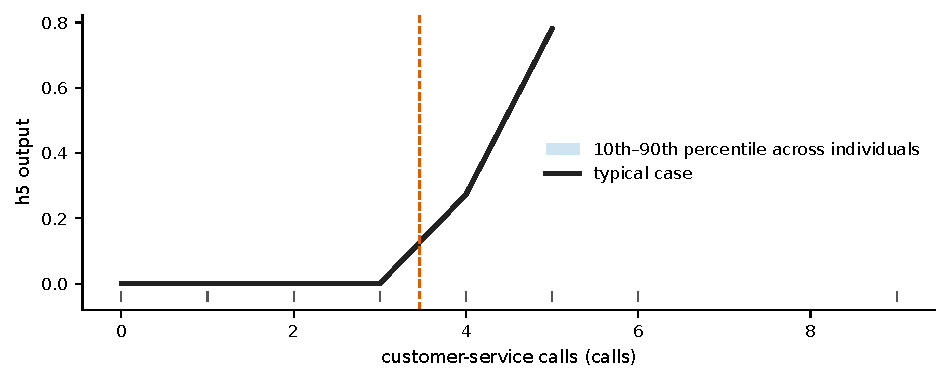
\includegraphics[width=\linewidth,height=0.88\textheight,keepaspectratio]{figures/churn100-s4-c2/ann_81-partial-6713.pdf}
\caption{Calls from 4 upwards: This part's own output, unit h5 (the output of 'Calls from 4 upwards'), on its own scale (its activation), with every other input at the typical case; it is active for 318 of 4000. Bold: the typical case; band: 10th to 90th percentile across individuals; dashed: where it switches on; ticks: the data.}
\label{fig:churn100s4c2:plot-ann81-1}
\end{figure}
\begin{figure}[H]\centering
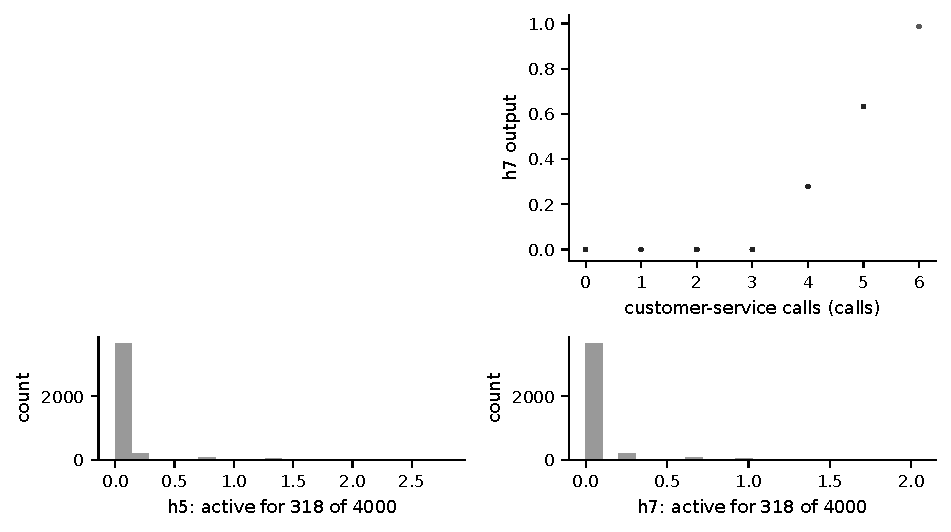
\includegraphics[width=\linewidth,height=0.88\textheight,keepaspectratio]{figures/churn100-s4-c2/ann_81-units.pdf}
\caption{Calls from 4 upwards: This part's hidden units: each unit's output against its main numeric input (top) and how often it is active (bottom).}
\label{fig:churn100s4c2:plot-ann81-2}
\end{figure}
\par\smallskip\noindent{\small Technical detail: \ref{tech:ann81}.\par}
\subsubsection{Calls from 3 upwards}\label{rd:ann80}
\noindent{\footnotesize Part of: Service calls (\ref{rd:ann86}).\par}
\noindent{\small Figure~\ref{fig:churn100s4c2:parts-ann80} shows what feeds this part; Figure~\ref{fig:churn100s4c2:units-ann80} its units and every connection into them (dashed boxes: connections from or to other parts, drawn in their own sections).\par}
\begin{figure}[H]\centering
\resizebox{!}{\ifdim\height>0.5\textheight 0.5\textheight\else\height\fi}{%
\resizebox{\ifdim\width>\linewidth\linewidth\else\width\fi}{!}{%
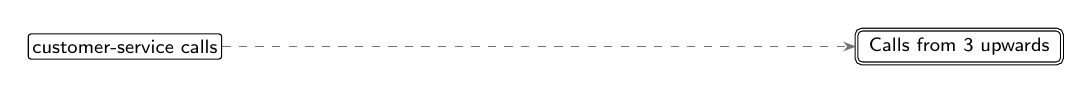
\begin{tikzpicture}[
  font=\sffamily\scriptsize, >={Stealth[length=1.6mm]},
  inp/.style={draw, rounded corners=1pt, fill=white, inner sep=1.5pt, minimum height=3.2mm, anchor=east},
  abox/.style={draw, thick, rounded corners=2pt, align=center, inner sep=3pt, minimum height=6mm, text width=42mm},
  outp/.style={draw, double, rounded corners=2pt, fill=white, align=center, inner sep=3pt, text width=24mm},
  agg/.style={draw=black!55},
]
\node[inp] (i0) at (0,-0.0) {customer-service calls};
\node[outp] (out) at (9.36,0) {Calls from 3 upwards};
\begin{scope}[on background layer]
\draw[->, agg, thin, dashed] (i0.east) -- (out.west);
\end{scope}
\end{tikzpicture}}}%
\caption{Calls from 3 upwards: what feeds it, one level down.}
\label{fig:churn100s4c2:parts-ann80}
\end{figure}
\begin{figure}[H]\centering
\resizebox{\ifdim\width>\linewidth\linewidth\else\width\fi}{!}{%
\definecolor{netup}{HTML}{D95F02}\definecolor{netdown}{HTML}{1B9E77}\definecolor{netmixed}{HTML}{7F7F7F}%
\begin{tikzpicture}[
  font=\sffamily\scriptsize, >={Stealth[length=1.4mm]},
  inp/.style={draw, circle, fill=white, minimum size=3.2mm, inner sep=0pt},
  hid/.style={draw, circle, fill=white, minimum size=5.2mm, inner sep=0.5pt, font=\sffamily\tiny},
  exitbox/.style={draw, thick, rectangle, fill=white, align=center, text width=17mm, minimum height=5mm, inner sep=1.5pt, font=\sffamily\tiny},
  sumbox/.style={draw, thick, dashed, rectangle, fill=white, align=center, text width=17mm, minimum height=5mm, inner sep=1.5pt, font=\sffamily\tiny},
  outp/.style={draw, thick, regular polygon, regular polygon sides=6, fill=white, minimum size=10mm, inner sep=0pt, font=\sffamily\tiny, align=center},
  stub/.style={draw, dashed, rounded corners=2pt, fill=white, align=center, inner sep=2pt, font=\sffamily\tiny, text width=15mm},
  inlab/.style={font=\sffamily\tiny, align=center, text width=15mm, inner sep=1pt, fill=white, fill opacity=0.8, text opacity=1},
  wpos/.style={draw=NavyBlue}, wneg/.style={draw=BrickRed}, wagg/.style={draw=black!45, line width=1.2pt},
  wmix/.style={draw=Plum},
]
\node[hid] (n12730) at (2.0,1.9) {h11};
\node[hid] (n12171) at (2.0,3.25) {h10};
\node[exitbox] (n5268) at (2.0,4.6) {Calls from 3 upwards $\uparrow$};
\node[inp, draw=netup, very thick] (ninxxnumberxcustomerxservicexcalls) at (2.0,0.0) {};
\path (ninxxnumberxcustomerxservicexcalls.south) node[inlab, anchor=north] (labninxxnumberxcustomerxservicexcalls) {customer-service calls $\uparrow$};
\node[stub] (ntoxxServicexcalls) at (2.0,6.15) {to Service calls};
\begin{scope}[on background layer]
\node[fit=(n12730) (n12171) (n5268) , inner sep=8pt, rounded corners=5pt, fill=ForestGreen!10, draw=ForestGreen!45] (clu0) {};
\draw[->, wpos, line width=0.38pt] (n12171) -- (n5268);
\draw[->, wpos, line width=0.50pt] (n12730) -- (n12171);
\draw[->, wpos, line width=0.34pt] (ninxxnumberxcustomerxservicexcalls) -- (n5268);
\draw[->, wpos, line width=0.55pt] (ninxxnumberxcustomerxservicexcalls) -- (n12171);
\draw[->, wpos, line width=0.53pt] (ninxxnumberxcustomerxservicexcalls) -- (n12730);
\draw[->, wpos, line width=0.83pt] (n5268) -- (ntoxxServicexcalls);
\end{scope}
\node[font=\sffamily\scriptsize\bfseries, text=ForestGreen!55!black, anchor=south west, inner sep=1pt, fill=white, fill opacity=0.85, text opacity=1] at (clu0.north west) {Calls from 3 upwards};
\end{tikzpicture}}%
\caption{Calls from 3 upwards: its units and every connection into them. Blue: positive weight (raises the score); red: negative weight (lowers it); thicker: larger weight. Orange outline and up arrow: raises the final prediction; teal and down arrow: lowers it; grey and double arrow: depends.}
\label{fig:churn100s4c2:units-ann80}
\end{figure}
\paragraph{Hypothesis.} This part raises the chance of leaving from 3 customer-service calls upwards, slowly at first, then faster.\,{\scriptsize\textcolor{NavyBlue}{[C097, C096]}}
\paragraph{Evidence.} It acts on 848 of 4000 training customers, 215 of whom left; for the typical customer it acts on, the chance is about 3\% without it and about 4\% with it.\,{\scriptsize\textcolor{NavyBlue}{[C098]}} Through it, the chance rises slowly at first, then faster: 4 calls take a typical such customer from about 3\% to about 8\%.\,{\scriptsize\textcolor{NavyBlue}{[C097]}} Its formula reproduces the part exactly on all 4000 training customers.\,{\scriptsize\textcolor{NavyBlue}{[C099]}}
\par\noindent{\small Evidence plots: Figure~\ref{fig:churn100s4c2:plot-ann80-0}, Figure~\ref{fig:churn100s4c2:plot-ann80-1}, Figure~\ref{fig:churn100s4c2:plot-ann80-2}.\par}
\par\noindent{\small Figure~\ref{fig:churn100s4c2:plot-ann80-1} shows this part's own output, unit h3: it switches on at about 2.805 calls of customer-service calls, and is zero below.\par}
\begin{figure}[H]\centering
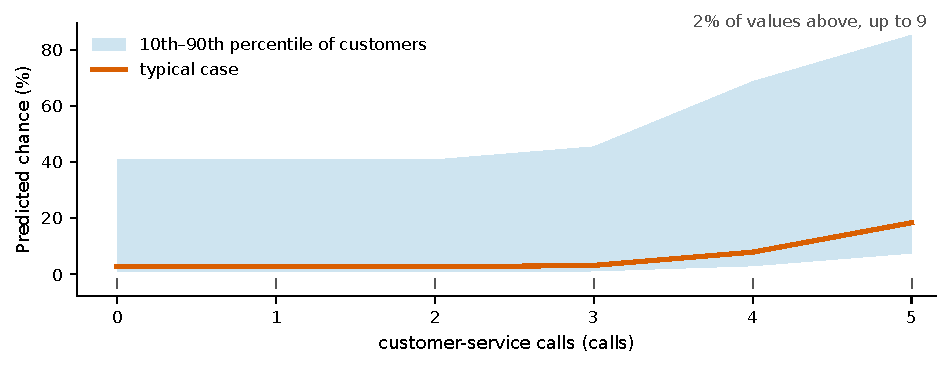
\includegraphics[width=\linewidth,height=0.88\textheight,keepaspectratio]{figures/churn100-s4-c2/ann_80-response.pdf}
\caption{Calls from 3 upwards: Response curves through this part: the typical case (bold), the 10th to 90th percentile of individual customers (band), the fold or step point (dashed) with its spread across them (grey), and the observed values (ticks).}
\label{fig:churn100s4c2:plot-ann80-0}
\end{figure}
\begin{figure}[H]\centering
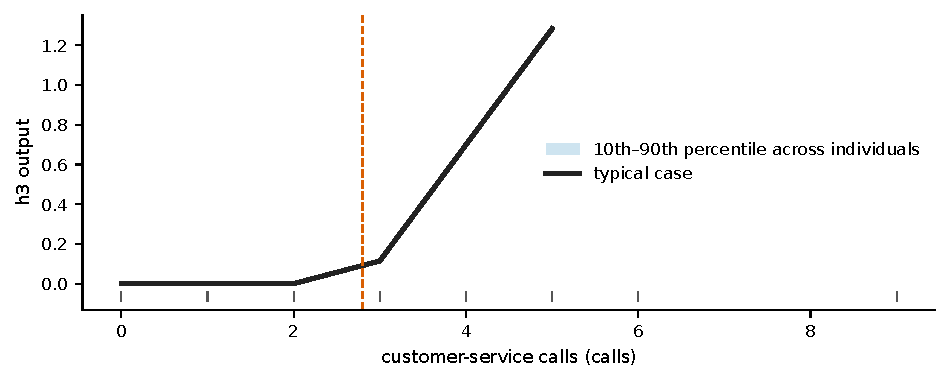
\includegraphics[width=\linewidth,height=0.88\textheight,keepaspectratio]{figures/churn100-s4-c2/ann_80-partial-5268.pdf}
\caption{Calls from 3 upwards: This part's own output, unit h3 (the output of 'Calls from 3 upwards'), on its own scale (its activation), with every other input at the typical case; it is active for 848 of 4000. Bold: the typical case; band: 10th to 90th percentile across individuals; dashed: where it switches on; ticks: the data.}
\label{fig:churn100s4c2:plot-ann80-1}
\end{figure}
\begin{figure}[H]\centering
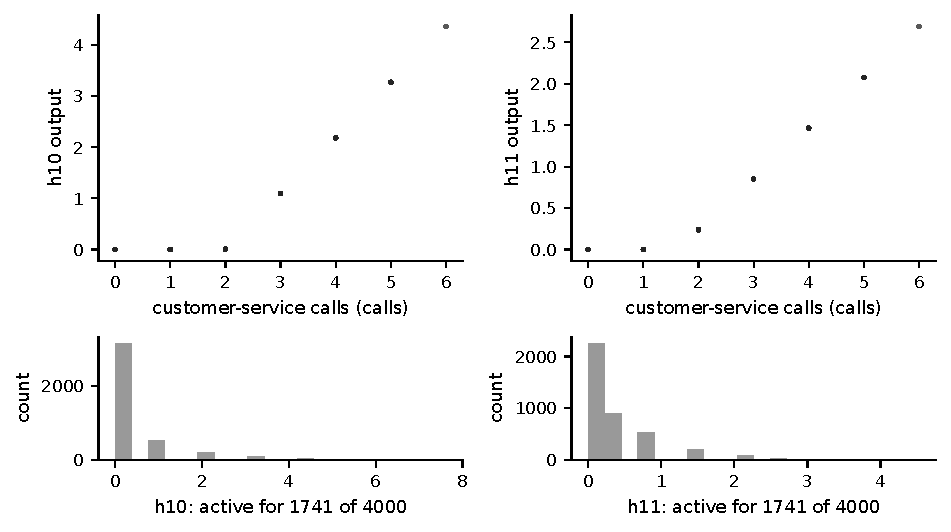
\includegraphics[width=\linewidth,height=0.88\textheight,keepaspectratio]{figures/churn100-s4-c2/ann_80-units.pdf}
\caption{Calls from 3 upwards: This part's hidden units: each unit's output against its main numeric input (top) and how often it is active (bottom).}
\label{fig:churn100s4c2:plot-ann80-2}
\end{figure}
\par\smallskip\noindent{\small Technical detail: \ref{tech:ann80}.\par}
\subsubsection{Heavy daytime use}\label{rd:ann82}
\noindent{\footnotesize Part of: The whole model (\ref{rd:ann87}).\par}
\noindent{\small Figure~\ref{fig:churn100s4c2:parts-ann82} shows what feeds this part; Figure~\ref{fig:churn100s4c2:units-ann82} its units and every connection into them (dashed boxes: connections from or to other parts, drawn in their own sections).\par}
\begin{figure}[H]\centering
\resizebox{!}{\ifdim\height>0.5\textheight 0.5\textheight\else\height\fi}{%
\resizebox{\ifdim\width>\linewidth\linewidth\else\width\fi}{!}{%
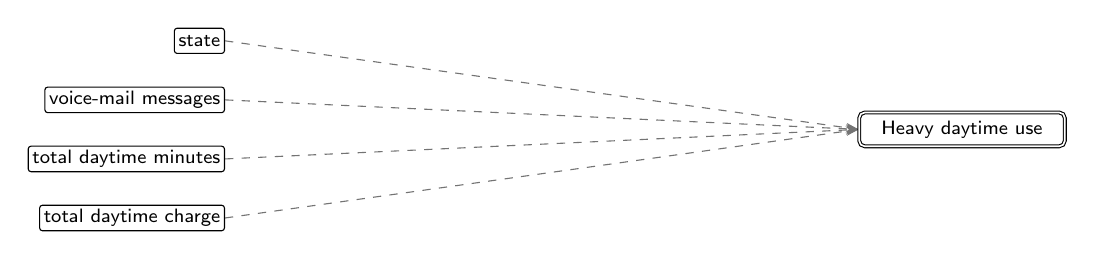
\begin{tikzpicture}[
  font=\sffamily\scriptsize, >={Stealth[length=1.6mm]},
  inp/.style={draw, rounded corners=1pt, fill=white, inner sep=1.5pt, minimum height=3.2mm, anchor=east},
  abox/.style={draw, thick, rounded corners=2pt, align=center, inner sep=3pt, minimum height=6mm, text width=42mm},
  outp/.style={draw, double, rounded corners=2pt, fill=white, align=center, inner sep=3pt, text width=24mm},
  agg/.style={draw=black!55},
]
\node[inp] (i0) at (0,1.125) {state};
\node[inp] (i1) at (0,0.375) {voice-mail messages};
\node[inp] (i2) at (0,-0.375) {total daytime minutes};
\node[inp] (i3) at (0,-1.125) {total daytime charge};
\node[outp] (out) at (9.36,0) {Heavy daytime use};
\begin{scope}[on background layer]
\draw[->, agg, thin, dashed] (i0.east) -- (out.west);
\draw[->, agg, thin, dashed] (i1.east) -- (out.west);
\draw[->, agg, thin, dashed] (i2.east) -- (out.west);
\draw[->, agg, thin, dashed] (i3.east) -- (out.west);
\end{scope}
\end{tikzpicture}}}%
\caption{Heavy daytime use: what feeds it, one level down.}
\label{fig:churn100s4c2:parts-ann82}
\end{figure}
\begin{figure}[H]\centering
\resizebox{\ifdim\width>\linewidth\linewidth\else\width\fi}{!}{%
\definecolor{netup}{HTML}{D95F02}\definecolor{netdown}{HTML}{1B9E77}\definecolor{netmixed}{HTML}{7F7F7F}%
\begin{tikzpicture}[
  font=\sffamily\scriptsize, >={Stealth[length=1.4mm]},
  inp/.style={draw, circle, fill=white, minimum size=3.2mm, inner sep=0pt},
  hid/.style={draw, circle, fill=white, minimum size=5.2mm, inner sep=0.5pt, font=\sffamily\tiny},
  exitbox/.style={draw, thick, rectangle, fill=white, align=center, text width=17mm, minimum height=5mm, inner sep=1.5pt, font=\sffamily\tiny},
  sumbox/.style={draw, thick, dashed, rectangle, fill=white, align=center, text width=17mm, minimum height=5mm, inner sep=1.5pt, font=\sffamily\tiny},
  outp/.style={draw, thick, regular polygon, regular polygon sides=6, fill=white, minimum size=10mm, inner sep=0pt, font=\sffamily\tiny, align=center},
  stub/.style={draw, dashed, rounded corners=2pt, fill=white, align=center, inner sep=2pt, font=\sffamily\tiny, text width=15mm},
  inlab/.style={font=\sffamily\tiny, align=center, text width=15mm, inner sep=1pt, fill=white, fill opacity=0.8, text opacity=1},
  wpos/.style={draw=NavyBlue}, wneg/.style={draw=BrickRed}, wagg/.style={draw=black!45, line width=1.2pt},
  wmix/.style={draw=Plum},
]
\node[hid] (n3118) at (4.35,1.9) {h2};
\node[hid] (n10131) at (2.85,1.9) {h9};
\node[inp, draw=netup, very thick] (ninxxtotalxdayxminutes) at (2.7,0.0) {};
\path (ninxxtotalxdayxminutes.south) node[inlab, anchor=north] (labninxxtotalxdayxminutes) {total daytime minutes $\uparrow$};
\node[inp, draw=netup, very thick] (ninxxtotalxdayxcharge) at (4.5,0.0) {};
\path (ninxxtotalxdayxcharge.south) node[inlab, anchor=north] (labninxxtotalxdayxcharge) {total daytime charge $\uparrow$};
\node[inp, draw=netdown, very thick] (ninxxnumberxvmailxmessages) at (6.3,0.0) {};
\path (ninxxnumberxvmailxmessages.south) node[inlab, anchor=north] (labninxxnumberxvmailxmessages) {voice-mail messages $\downarrow$};
\node[inp, draw=netmixed, very thick] (ngrpxxstate) at (0.9,0.0) {};
\path (ngrpxxstate.south) node[inlab, anchor=north] (labngrpxxstate) {state (22 of 51 used) $\updownarrow$};
\node[stub] (ntoxxthexmodelxoutput) at (3.6,3.45) {to the model output};
\begin{scope}[on background layer]
\node[fit=(n3118) (n10131) , inner sep=8pt, rounded corners=5pt, fill=Orchid!10, draw=Orchid!45] (clu0) {};
\draw[->, wpos, line width=0.44pt] (ninxxtotalxdayxminutes) -- (n3118);
\draw[->, wpos, line width=0.38pt] (ninxxtotalxdayxcharge) -- (n3118);
\draw[->, wpos, line width=0.54pt] (ninxxtotalxdayxminutes) -- (n10131);
\draw[->, wneg, line width=0.48pt] (ninxxnumberxvmailxmessages) -- (n3118);
\draw[->, wpos, line width=0.79pt] (n3118) -- (ntoxxthexmodelxoutput);
\draw[->, wpos, line width=0.92pt] (n10131) -- (ntoxxthexmodelxoutput);
\draw[->, wneg, line width=0.49pt] (ngrpxxstate) -- node[pos=0.8, sloped, above, font=\sffamily\tiny, inner sep=1pt, fill=white, fill opacity=0.8, text opacity=1] {-0.67} (n10131);
\end{scope}
\node[font=\sffamily\scriptsize\bfseries, text=Orchid!55!black, anchor=south west, inner sep=1pt, fill=white, fill opacity=0.85, text opacity=1] at (clu0.north west) {Heavy daytime use};
\end{tikzpicture}}%
\caption{Heavy daytime use: its units and every connection into them. Blue: positive weight (raises the score); red: negative weight (lowers it); thicker: larger weight. Orange outline and up arrow: raises the final prediction; teal and down arrow: lowers it; grey and double arrow: depends.}
\label{fig:churn100s4c2:units-ann82}
\end{figure}
\paragraph{Hypothesis.} This part raises the chance of leaving for heavy daytime users: daytime minutes add to it only above about 221 minutes (between 186 and 221 minutes for different customers), in an uneven way, and voice-mail messages and being in Washington lower it.\,{\scriptsize\textcolor{NavyBlue}{[C088, C080, C082]}}
\paragraph{Evidence.} This part acts on 1099 of 4000 training customers, 291 of whom left; for the typical customer it acts on, the chance is about 3\% without it and about 12\% with it.\,{\scriptsize\textcolor{NavyBlue}{[C091]}} Daytime minutes add to the chance only once they rise above about 221 minutes (between 186 and 221 minutes for different customers), in an uneven way: for a typical such customer, from about 3\% at 0 minutes to about 19\% at 271 minutes.\,{\scriptsize\textcolor{NavyBlue}{[C088]}} More voice-mail messages lower it in an uneven way: for the typical customer it acts on, from about 12\% at 0 to about 6\% at 32 messages.\,{\scriptsize\textcolor{NavyBlue}{[C080]}} Customers in Washington get less from it: about 7\% instead of about 12\% for the typical customer it acts on.\,{\scriptsize\textcolor{NavyBlue}{[C082]}} Its formula reproduces the part exactly on all 4000 training customers.\,{\scriptsize\textcolor{NavyBlue}{[C092]}}
\par\noindent{\small Evidence plots: Figure~\ref{fig:churn100s4c2:plot-ann82-0}, Figure~\ref{fig:churn100s4c2:plot-ann82-1}, Figure~\ref{fig:churn100s4c2:plot-ann82-2}, Figure~\ref{fig:churn100s4c2:plot-ann82-3}, Figure~\ref{fig:churn100s4c2:plot-ann82-4}, Figure~\ref{fig:churn100s4c2:plot-ann82-5}, Figure~\ref{fig:churn100s4c2:plot-ann82-6}, Figure~\ref{fig:churn100s4c2:plot-ann82-7}, Figure~\ref{fig:churn100s4c2:plot-ann82-8}.\par}
\par\noindent{\small Figure~\ref{fig:churn100s4c2:plot-ann82-6} shows this part's own output, unit h2: over its two main inputs, with the line where it switches on.\par}
\par\noindent{\small Figure~\ref{fig:churn100s4c2:plot-ann82-7} shows this part's own output, unit h9: it switches on at about 221.1 minutes of total daytime minutes, and is zero below.\par}
\begin{figure}[H]\centering
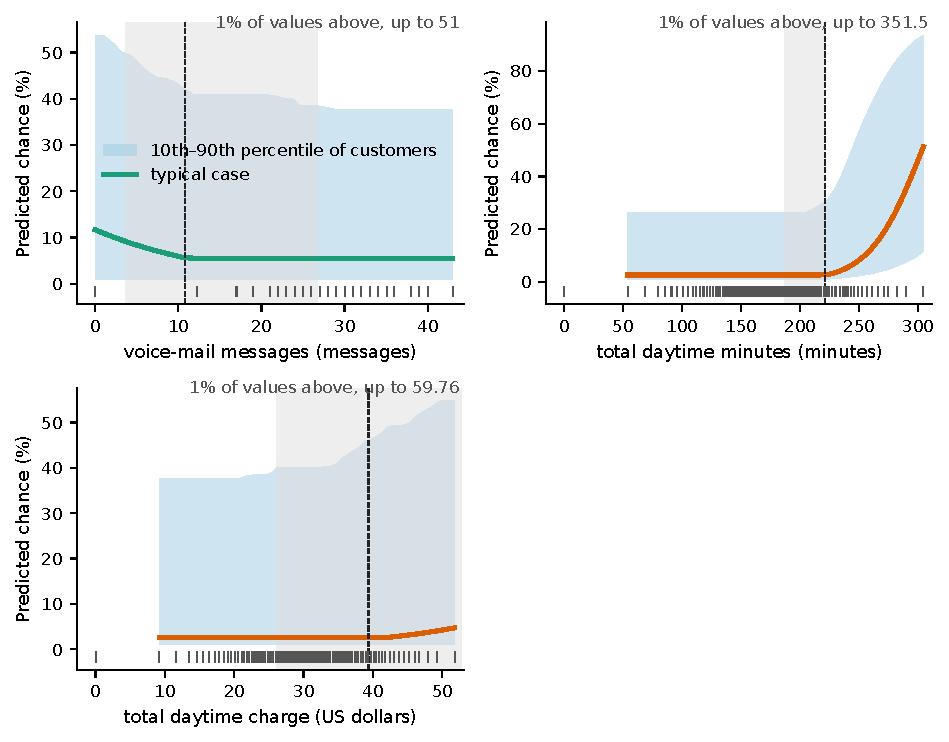
\includegraphics[width=\linewidth,height=0.88\textheight,keepaspectratio]{figures/churn100-s4-c2/ann_82-response.pdf}
\caption{Heavy daytime use: Response curves through this part: the typical case (bold), the 10th to 90th percentile of individual customers (band), the fold or step point (dashed) with its spread across them (grey), and the observed values (ticks).}
\label{fig:churn100s4c2:plot-ann82-0}
\end{figure}
\begin{figure}[H]\centering
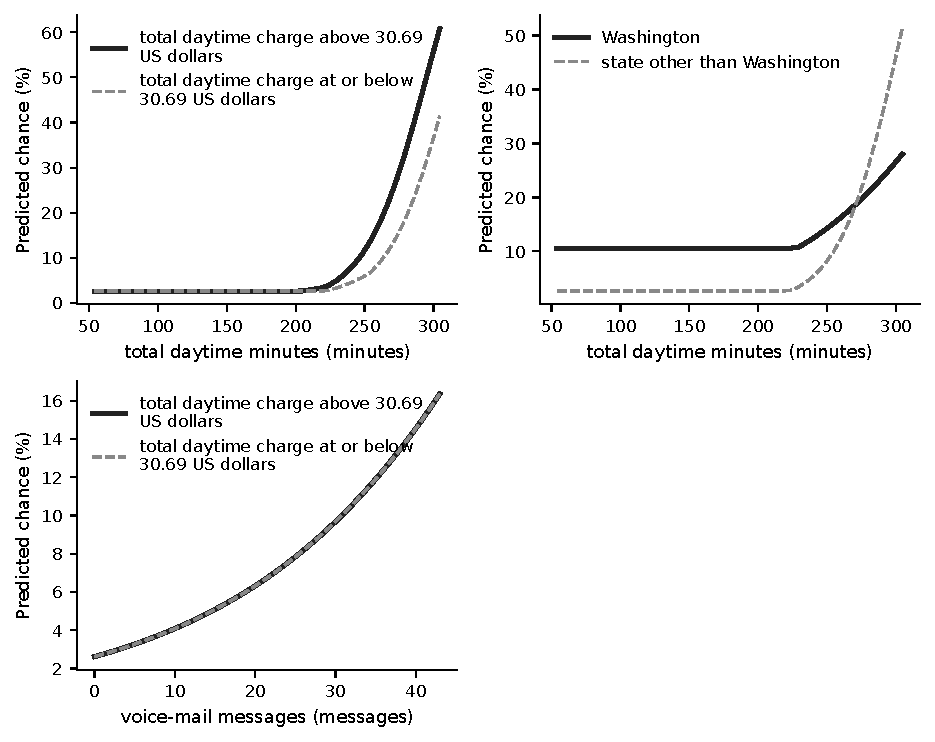
\includegraphics[width=\linewidth,height=0.88\textheight,keepaspectratio]{figures/churn100-s4-c2/ann_82-interaction.pdf}
\caption{Heavy daytime use: How the effect differs between groups: one curve per group, for the typical case of each group.}
\label{fig:churn100s4c2:plot-ann82-1}
\end{figure}
\begin{figure}[H]\centering
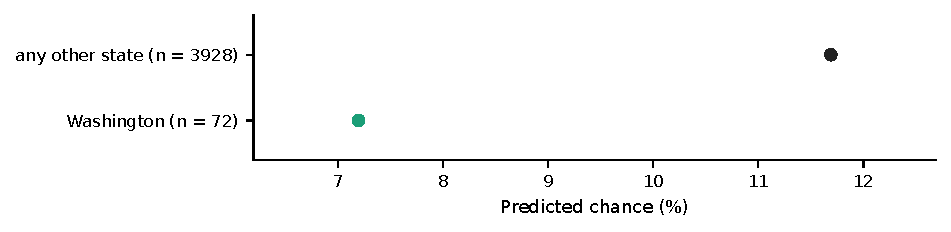
\includegraphics[width=\linewidth,height=0.88\textheight,keepaspectratio]{figures/churn100-s4-c2/ann_82-categories-small.pdf}
\caption{Heavy daytime use: The predicted value for the typical case at each level, through this part (n = training customers; grey: fewer than 20).}
\label{fig:churn100s4c2:plot-ann82-2}
\end{figure}
\begin{figure}[H]\centering
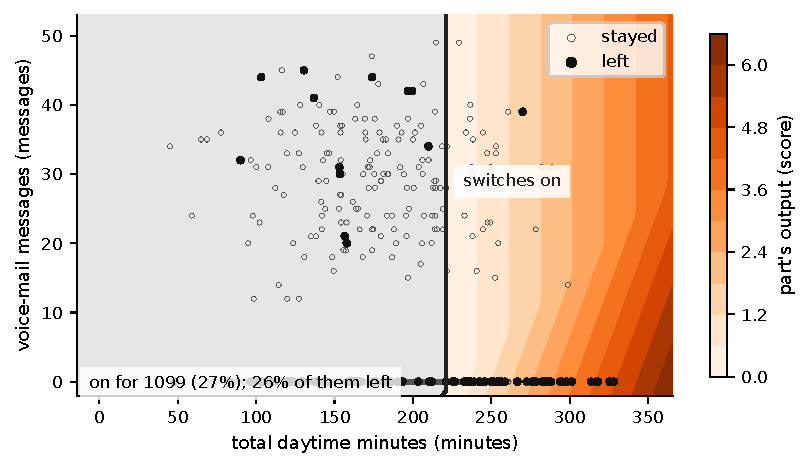
\includegraphics[width=\linewidth,height=0.88\textheight,keepaspectratio]{figures/churn100-s4-c2/ann_82-deep-map.pdf}
\caption{Heavy daytime use: The part's own output over its two numeric inputs, other inputs at the typical case: colour where it is on, flat grey where it is switched off, the black line where it switches on; training customers as hollow (no event) and filled (event) points, so the part can be seen catching the events (the predicted-chance overlay was harder to read). The switch-on line is traced on this map only; the boundary claim (C113) did not pass its check on the data, so no rule is stated.}
\label{fig:churn100s4c2:plot-ann82-3}
\end{figure}
\begin{figure}[H]\centering
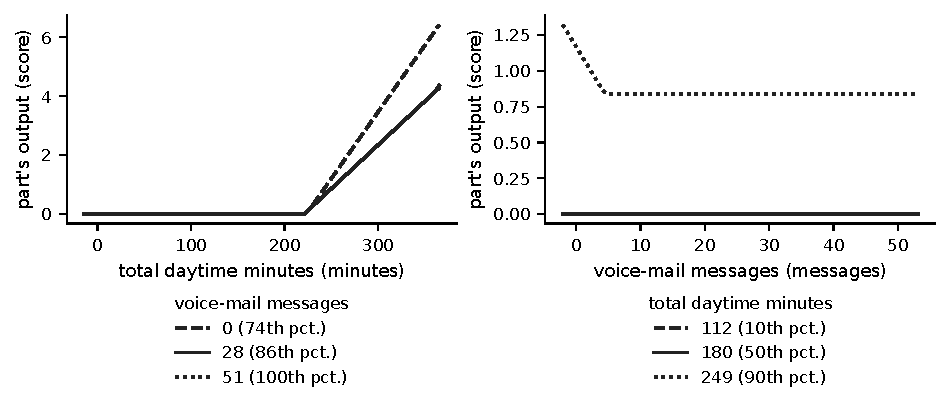
\includegraphics[width=\linewidth,height=0.88\textheight,keepaspectratio]{figures/churn100-s4-c2/ann_82-deep-slices.pdf}
\caption{Heavy daytime use: Slices of the same map: the part's own output against each input at three values of the other, so the tilted boundary shows as a shifting hinge. The switch-on line is traced on this map only; the boundary claim (C113) did not pass its check on the data, so no rule is stated.}
\label{fig:churn100s4c2:plot-ann82-4}
\end{figure}
\begin{figure}[H]\centering
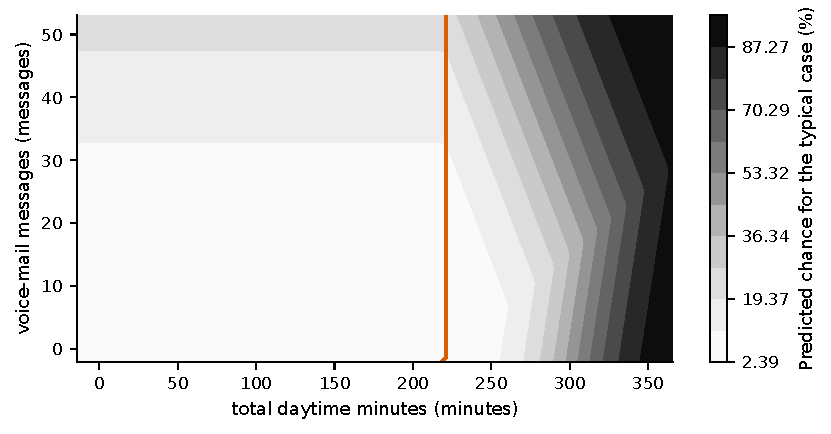
\includegraphics[width=\linewidth,height=0.88\textheight,keepaspectratio]{figures/churn100-s4-c2/ann_82-deep-risk.pdf}
\caption{Heavy daytime use: The same map on the final scale: the predicted value for the typical case, with the switch-on line (orange). The switch-on line is traced on this map only; the boundary claim (C113) did not pass its check on the data, so no rule is stated.}
\label{fig:churn100s4c2:plot-ann82-5}
\end{figure}
\begin{figure}[H]\centering
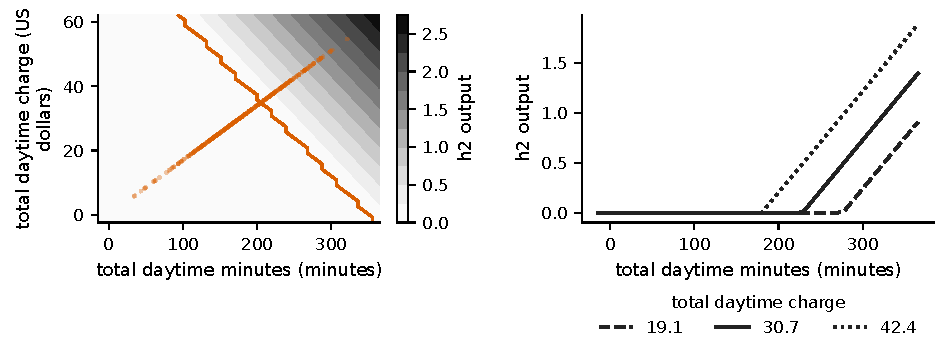
\includegraphics[width=\linewidth,height=0.88\textheight,keepaspectratio]{figures/churn100-s4-c2/ann_82-partial-3118.pdf}
\caption{Heavy daytime use: This part's own output, unit h2 (the output of 'Heavy daytime use'), on its own scale (its activation), with every other input at the typical case; it is active for 896 of 4000. Left: its output over its two main inputs (orange line: where it switches on; dots: the data); right: slices at three values of the second input.}
\label{fig:churn100s4c2:plot-ann82-6}
\end{figure}
\begin{figure}[H]\centering
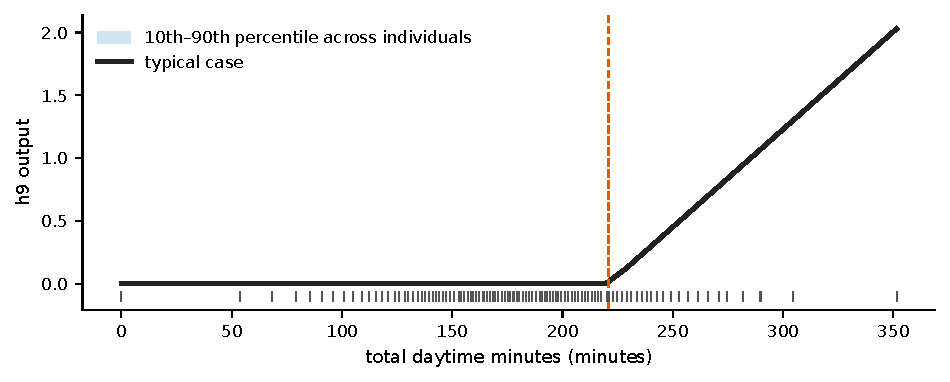
\includegraphics[width=\linewidth,height=0.88\textheight,keepaspectratio]{figures/churn100-s4-c2/ann_82-partial-10131.pdf}
\caption{Heavy daytime use: This part's own output, unit h9 (the output of 'Heavy daytime use'), on its own scale (its activation), with every other input at the typical case; it is active for 870 of 4000. Bold: the typical case; band: 10th to 90th percentile across individuals; dashed: where it switches on; ticks: the data.}
\label{fig:churn100s4c2:plot-ann82-7}
\end{figure}
\begin{figure}[H]\centering
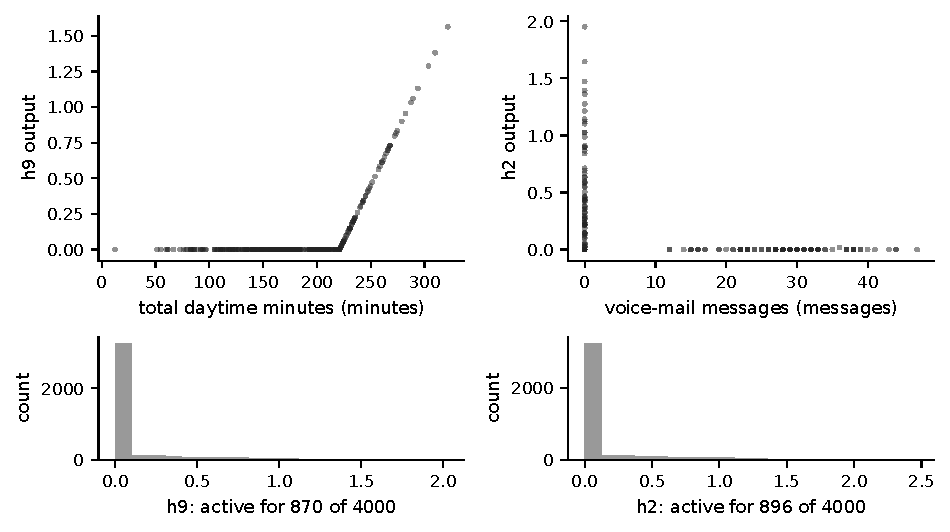
\includegraphics[width=\linewidth,height=0.88\textheight,keepaspectratio]{figures/churn100-s4-c2/ann_82-units.pdf}
\caption{Heavy daytime use: This part's hidden units: each unit's output against its main numeric input (top) and how often it is active (bottom).}
\label{fig:churn100s4c2:plot-ann82-8}
\end{figure}
\par\smallskip\noindent{\small Technical detail: \ref{tech:ann82}.\par}
\subsubsection{State units}\label{rd:ann85}
\noindent{\footnotesize Part of: The whole model (\ref{rd:ann87}).\par}
\noindent{\small Figure~\ref{fig:churn100s4c2:parts-ann85} shows what feeds this part; Figure~\ref{fig:churn100s4c2:units-ann85} its units and every connection into them (dashed boxes: connections from or to other parts, drawn in their own sections).\par}
\begin{figure}[H]\centering
\resizebox{!}{\ifdim\height>0.5\textheight 0.5\textheight\else\height\fi}{%
\resizebox{\ifdim\width>\linewidth\linewidth\else\width\fi}{!}{%
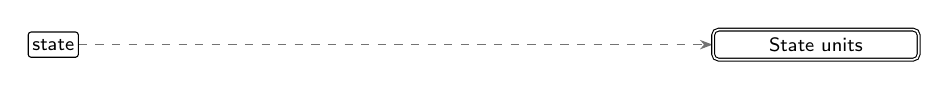
\begin{tikzpicture}[
  font=\sffamily\scriptsize, >={Stealth[length=1.6mm]},
  inp/.style={draw, rounded corners=1pt, fill=white, inner sep=1.5pt, minimum height=3.2mm, anchor=east},
  abox/.style={draw, thick, rounded corners=2pt, align=center, inner sep=3pt, minimum height=6mm, text width=42mm},
  outp/.style={draw, double, rounded corners=2pt, fill=white, align=center, inner sep=3pt, text width=24mm},
  agg/.style={draw=black!55},
]
\node[inp] (i0) at (0,-0.0) {state};
\node[outp] (out) at (9.36,0) {State units};
\begin{scope}[on background layer]
\draw[->, agg, thin, dashed] (i0.east) -- (out.west);
\end{scope}
\end{tikzpicture}}}%
\caption{State units: what feeds it, one level down.}
\label{fig:churn100s4c2:parts-ann85}
\end{figure}
\begin{figure}[H]\centering
\resizebox{\ifdim\width>\linewidth\linewidth\else\width\fi}{!}{%
\definecolor{netup}{HTML}{D95F02}\definecolor{netdown}{HTML}{1B9E77}\definecolor{netmixed}{HTML}{7F7F7F}%
\begin{tikzpicture}[
  font=\sffamily\scriptsize, >={Stealth[length=1.4mm]},
  inp/.style={draw, circle, fill=white, minimum size=3.2mm, inner sep=0pt},
  hid/.style={draw, circle, fill=white, minimum size=5.2mm, inner sep=0.5pt, font=\sffamily\tiny},
  exitbox/.style={draw, thick, rectangle, fill=white, align=center, text width=17mm, minimum height=5mm, inner sep=1.5pt, font=\sffamily\tiny},
  sumbox/.style={draw, thick, dashed, rectangle, fill=white, align=center, text width=17mm, minimum height=5mm, inner sep=1.5pt, font=\sffamily\tiny},
  outp/.style={draw, thick, regular polygon, regular polygon sides=6, fill=white, minimum size=10mm, inner sep=0pt, font=\sffamily\tiny, align=center},
  stub/.style={draw, dashed, rounded corners=2pt, fill=white, align=center, inner sep=2pt, font=\sffamily\tiny, text width=15mm},
  inlab/.style={font=\sffamily\tiny, align=center, text width=15mm, inner sep=1pt, fill=white, fill opacity=0.8, text opacity=1},
  wpos/.style={draw=NavyBlue}, wneg/.style={draw=BrickRed}, wagg/.style={draw=black!45, line width=1.2pt},
  wmix/.style={draw=Plum},
]
\node[hid] (n9954) at (1.85,1.9) {h8};
\node[hid] (n1295) at (0.35,1.9) {h1};
\node[hid] (n7872) at (1.1,3.25) {h6};
\node[inp, draw=netmixed, very thick] (ngrpxxstate) at (1.1,0.0) {};
\path (ngrpxxstate.south) node[inlab, anchor=north] (labngrpxxstate) {state (22 of 51 used) $\updownarrow$};
\node[stub] (ntoxxthexmodelxoutput) at (1.1,4.8) {to the model output};
\begin{scope}[on background layer]
\node[fit=(n9954) (n1295) (n7872) , inner sep=8pt, rounded corners=5pt, fill=Goldenrod!10, draw=Goldenrod!45] (clu0) {};
\draw[->, wpos, line width=0.61pt] (n1295) -- (n7872);
\draw[->, wneg, line width=0.60pt] (n1295) -- (ntoxxthexmodelxoutput);
\draw[->, wneg, line width=0.67pt] (n7872) -- (ntoxxthexmodelxoutput);
\draw[->, wpos, line width=0.26pt] (n9954) -- (ntoxxthexmodelxoutput);
\draw[->, wpos, line width=0.60pt] (ngrpxxstate) -- node[pos=0.8, sloped, above, font=\sffamily\tiny, inner sep=1pt, fill=white, fill opacity=0.8, text opacity=1] {+1.01} (n9954);
\draw[->, wneg, line width=0.69pt] (ngrpxxstate) -- node[pos=0.8, sloped, above, font=\sffamily\tiny, inner sep=1pt, fill=white, fill opacity=0.8, text opacity=1] {-1.27} (n1295);
\end{scope}
\node[font=\sffamily\scriptsize\bfseries, text=Goldenrod!55!black, anchor=south west, inner sep=1pt, fill=white, fill opacity=0.85, text opacity=1] at (clu0.north west) {State units};
\end{tikzpicture}}%
\caption{State units: its units and every connection into them. Blue: positive weight (raises the score); red: negative weight (lowers it); thicker: larger weight. Orange outline and up arrow: raises the final prediction; teal and down arrow: lowers it; grey and double arrow: depends.}
\label{fig:churn100s4c2:units-ann85}
\end{figure}
\paragraph{Hypothesis.} This part reads only the state and raises the chance of leaving in Rhode Island, and a little in Indiana.\,{\scriptsize\textcolor{NavyBlue}{[C100, C101]}}
\paragraph{Evidence.} Through it, a typical customer's chance goes from about 3\% to about 22\% in Rhode Island, and up by less than a point in Indiana.\,{\scriptsize\textcolor{NavyBlue}{[C100, C101]}} Its formula reproduces the part exactly on all 4000 training customers.\,{\scriptsize\textcolor{NavyBlue}{[C102]}}
\par\noindent{\small Evidence plots: Figure~\ref{fig:churn100s4c2:plot-ann85-0}, Figure~\ref{fig:churn100s4c2:plot-ann85-1}.\par}
\begin{figure}[H]\centering
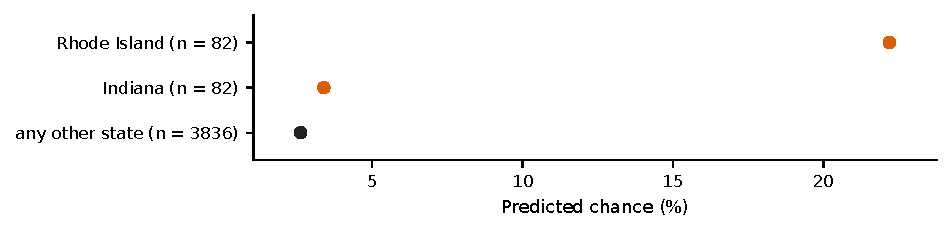
\includegraphics[width=\linewidth,height=0.88\textheight,keepaspectratio]{figures/churn100-s4-c2/ann_85-categories-small.pdf}
\caption{State units: The predicted value for the typical case at each level, through this part (n = training customers; grey: fewer than 20).}
\label{fig:churn100s4c2:plot-ann85-0}
\end{figure}
\begin{figure}[H]\centering
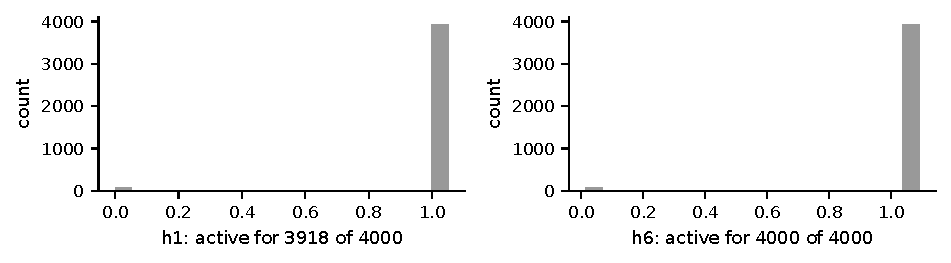
\includegraphics[width=\linewidth,height=0.88\textheight,keepaspectratio]{figures/churn100-s4-c2/ann_85-units.pdf}
\caption{State units: This part's hidden units: each unit's output against its main numeric input (top) and how often it is active (bottom).}
\label{fig:churn100s4c2:plot-ann85-1}
\end{figure}
\par\smallskip\noindent{\small Technical detail: \ref{tech:ann85}.\par}
\subsubsection{Evening unit}\label{rd:ann83}
\noindent{\footnotesize Part of: The whole model (\ref{rd:ann87}).\par}
\noindent{\small Figure~\ref{fig:churn100s4c2:parts-ann83} shows what feeds this part; Figure~\ref{fig:churn100s4c2:units-ann83} its units and every connection into them (dashed boxes: connections from or to other parts, drawn in their own sections).\par}
\begin{figure}[H]\centering
\resizebox{!}{\ifdim\height>0.5\textheight 0.5\textheight\else\height\fi}{%
\resizebox{\ifdim\width>\linewidth\linewidth\else\width\fi}{!}{%
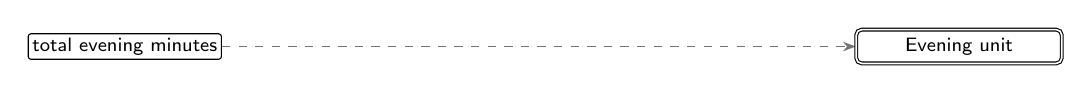
\begin{tikzpicture}[
  font=\sffamily\scriptsize, >={Stealth[length=1.6mm]},
  inp/.style={draw, rounded corners=1pt, fill=white, inner sep=1.5pt, minimum height=3.2mm, anchor=east},
  abox/.style={draw, thick, rounded corners=2pt, align=center, inner sep=3pt, minimum height=6mm, text width=42mm},
  outp/.style={draw, double, rounded corners=2pt, fill=white, align=center, inner sep=3pt, text width=24mm},
  agg/.style={draw=black!55},
]
\node[inp] (i0) at (0,-0.0) {total evening minutes};
\node[outp] (out) at (9.36,0) {Evening unit};
\begin{scope}[on background layer]
\draw[->, agg, thin, dashed] (i0.east) -- (out.west);
\end{scope}
\end{tikzpicture}}}%
\caption{Evening unit: what feeds it, one level down.}
\label{fig:churn100s4c2:parts-ann83}
\end{figure}
\begin{figure}[H]\centering
\resizebox{\ifdim\width>\linewidth\linewidth\else\width\fi}{!}{%
\definecolor{netup}{HTML}{D95F02}\definecolor{netdown}{HTML}{1B9E77}\definecolor{netmixed}{HTML}{7F7F7F}%
\begin{tikzpicture}[
  font=\sffamily\scriptsize, >={Stealth[length=1.4mm]},
  inp/.style={draw, circle, fill=white, minimum size=3.2mm, inner sep=0pt},
  hid/.style={draw, circle, fill=white, minimum size=5.2mm, inner sep=0.5pt, font=\sffamily\tiny},
  exitbox/.style={draw, thick, rectangle, fill=white, align=center, text width=17mm, minimum height=5mm, inner sep=1.5pt, font=\sffamily\tiny},
  sumbox/.style={draw, thick, dashed, rectangle, fill=white, align=center, text width=17mm, minimum height=5mm, inner sep=1.5pt, font=\sffamily\tiny},
  outp/.style={draw, thick, regular polygon, regular polygon sides=6, fill=white, minimum size=10mm, inner sep=0pt, font=\sffamily\tiny, align=center},
  stub/.style={draw, dashed, rounded corners=2pt, fill=white, align=center, inner sep=2pt, font=\sffamily\tiny, text width=15mm},
  inlab/.style={font=\sffamily\tiny, align=center, text width=15mm, inner sep=1pt, fill=white, fill opacity=0.8, text opacity=1},
  wpos/.style={draw=NavyBlue}, wneg/.style={draw=BrickRed}, wagg/.style={draw=black!45, line width=1.2pt},
  wmix/.style={draw=Plum},
]
\node[exitbox] (n15524) at (1.2,3.25) {Evening unit $\uparrow$};
\node[hid] (n14484) at (1.2,1.9) {h12};
\node[inp, draw=netup, very thick] (ninxxtotalxevexminutes) at (1.2,0.0) {};
\path (ninxxtotalxevexminutes.south) node[inlab, anchor=north] (labninxxtotalxevexminutes) {total evening minutes $\uparrow$};
\node[stub] (ntoxxthexmodelxoutput) at (1.2,4.8) {to the model output};
\begin{scope}[on background layer]
\node[fit=(n15524) (n14484) , inner sep=8pt, rounded corners=5pt, fill=Cerulean!10, draw=Cerulean!45] (clu0) {};
\draw[->, wpos, line width=0.60pt] (ninxxtotalxevexminutes) -- (n14484);
\draw[->, wpos, line width=0.61pt] (n14484) -- (n15524);
\draw[->, wpos, line width=0.32pt] (n15524) -- (ntoxxthexmodelxoutput);
\end{scope}
\node[font=\sffamily\scriptsize\bfseries, text=Cerulean!55!black, anchor=south west, inner sep=1pt, fill=white, fill opacity=0.85, text opacity=1] at (clu0.north west) {Evening unit};
\end{tikzpicture}}%
\caption{Evening unit: its units and every connection into them. Blue: positive weight (raises the score); red: negative weight (lowers it); thicker: larger weight. Orange outline and up arrow: raises the final prediction; teal and down arrow: lowers it; grey and double arrow: depends.}
\label{fig:churn100s4c2:units-ann83}
\end{figure}
\paragraph{Hypothesis.} This part reads evening minutes and barely changes the chance of leaving: nothing until about 217 minutes, then steadily.\,{\scriptsize\textcolor{NavyBlue}{[C103, C104]}}
\paragraph{Evidence.} Through it, evening minutes change nothing until about 217 minutes, then raise the chance steadily, but a typical customer's chance stays at about 3\% from 138 to 266 minutes.\,{\scriptsize\textcolor{NavyBlue}{[C103]}} Its formula reproduces the part exactly on all 4000 training customers.\,{\scriptsize\textcolor{NavyBlue}{[C105]}}
\par\noindent{\small Evidence plots: Figure~\ref{fig:churn100s4c2:plot-ann83-0}, Figure~\ref{fig:churn100s4c2:plot-ann83-1}.\par}
\begin{figure}[H]\centering
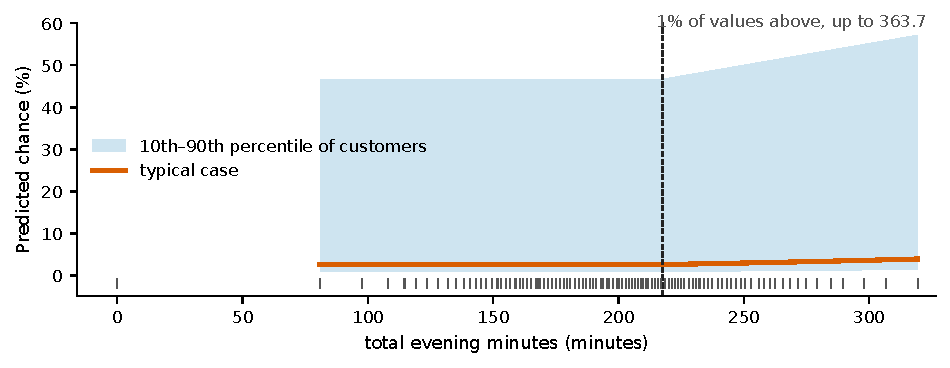
\includegraphics[width=\linewidth,height=0.88\textheight,keepaspectratio]{figures/churn100-s4-c2/ann_83-response.pdf}
\caption{Evening unit: Response curves through this part: the typical case (bold), the 10th to 90th percentile of individual customers (band), the fold or step point (dashed) with its spread across them (grey), and the observed values (ticks).}
\label{fig:churn100s4c2:plot-ann83-0}
\end{figure}
\begin{figure}[H]\centering
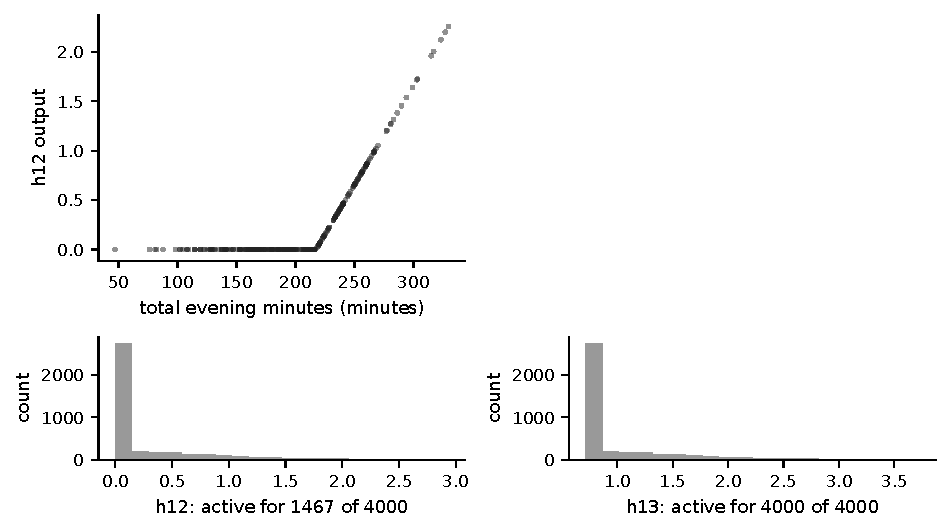
\includegraphics[width=\linewidth,height=0.88\textheight,keepaspectratio]{figures/churn100-s4-c2/ann_83-units.pdf}
\caption{Evening unit: This part's hidden units: each unit's output against its main numeric input (top) and how often it is active (bottom).}
\label{fig:churn100s4c2:plot-ann83-1}
\end{figure}
\par\smallskip\noindent{\small Technical detail: \ref{tech:ann83}.\par}
\subsubsection{Small voice-mail unit}\label{rd:ann84}
\noindent{\footnotesize Part of: The whole model (\ref{rd:ann87}).\par}
\noindent{\small Figure~\ref{fig:churn100s4c2:parts-ann84} shows what feeds this part; Figure~\ref{fig:churn100s4c2:units-ann84} its units and every connection into them (dashed boxes: connections from or to other parts, drawn in their own sections).\par}
\begin{figure}[H]\centering
\resizebox{!}{\ifdim\height>0.5\textheight 0.5\textheight\else\height\fi}{%
\resizebox{\ifdim\width>\linewidth\linewidth\else\width\fi}{!}{%
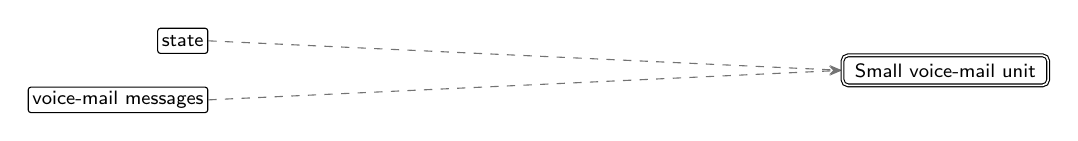
\begin{tikzpicture}[
  font=\sffamily\scriptsize, >={Stealth[length=1.6mm]},
  inp/.style={draw, rounded corners=1pt, fill=white, inner sep=1.5pt, minimum height=3.2mm, anchor=east},
  abox/.style={draw, thick, rounded corners=2pt, align=center, inner sep=3pt, minimum height=6mm, text width=42mm},
  outp/.style={draw, double, rounded corners=2pt, fill=white, align=center, inner sep=3pt, text width=24mm},
  agg/.style={draw=black!55},
]
\node[inp] (i0) at (0,0.375) {state};
\node[inp] (i1) at (0,-0.375) {voice-mail messages};
\node[outp] (out) at (9.36,0) {Small voice-mail unit};
\begin{scope}[on background layer]
\draw[->, agg, thin, dashed] (i0.east) -- (out.west);
\draw[->, agg, thin, dashed] (i1.east) -- (out.west);
\end{scope}
\end{tikzpicture}}}%
\caption{Small voice-mail unit: what feeds it, one level down.}
\label{fig:churn100s4c2:parts-ann84}
\end{figure}
\begin{figure}[H]\centering
\resizebox{\ifdim\width>\linewidth\linewidth\else\width\fi}{!}{%
\definecolor{netup}{HTML}{D95F02}\definecolor{netdown}{HTML}{1B9E77}\definecolor{netmixed}{HTML}{7F7F7F}%
\begin{tikzpicture}[
  font=\sffamily\scriptsize, >={Stealth[length=1.4mm]},
  inp/.style={draw, circle, fill=white, minimum size=3.2mm, inner sep=0pt},
  hid/.style={draw, circle, fill=white, minimum size=5.2mm, inner sep=0.5pt, font=\sffamily\tiny},
  exitbox/.style={draw, thick, rectangle, fill=white, align=center, text width=17mm, minimum height=5mm, inner sep=1.5pt, font=\sffamily\tiny},
  sumbox/.style={draw, thick, dashed, rectangle, fill=white, align=center, text width=17mm, minimum height=5mm, inner sep=1.5pt, font=\sffamily\tiny},
  outp/.style={draw, thick, regular polygon, regular polygon sides=6, fill=white, minimum size=10mm, inner sep=0pt, font=\sffamily\tiny, align=center},
  stub/.style={draw, dashed, rounded corners=2pt, fill=white, align=center, inner sep=2pt, font=\sffamily\tiny, text width=15mm},
  inlab/.style={font=\sffamily\tiny, align=center, text width=15mm, inner sep=1pt, fill=white, fill opacity=0.8, text opacity=1},
  wpos/.style={draw=NavyBlue}, wneg/.style={draw=BrickRed}, wagg/.style={draw=black!45, line width=1.2pt},
  wmix/.style={draw=Plum},
]
\node[exitbox] (n6089) at (2.1,1.9) {Small voice-mail unit $\uparrow$};
\node[inp, draw=netup, very thick] (ninxxnumberxvmailxmessages) at (3.0,0.0) {};
\path (ninxxnumberxvmailxmessages.south) node[inlab, anchor=north] (labninxxnumberxvmailxmessages) {voice-mail messages $\uparrow$};
\node[inp, draw=netmixed, very thick] (ngrpxxstate) at (1.2,0.0) {};
\path (ngrpxxstate.south) node[inlab, anchor=north] (labngrpxxstate) {state (22 of 51 used) $\updownarrow$};
\node[stub] (ntoxxthexmodelxoutput) at (2.1,3.45) {to the model output};
\begin{scope}[on background layer]
\node[fit=(n6089) , inner sep=8pt, rounded corners=5pt, fill=Mahogany!10, draw=Mahogany!45] (clu0) {};
\draw[->, wpos, line width=0.54pt] (ninxxnumberxvmailxmessages) -- (n6089);
\draw[->, wpos, line width=0.25pt] (n6089) -- (ntoxxthexmodelxoutput);
\draw[->, wpos, line width=0.65pt] (ngrpxxstate) -- node[pos=0.8, sloped, above, font=\sffamily\tiny, inner sep=1pt, fill=white, fill opacity=0.8, text opacity=1] {+1.14} (n6089);
\end{scope}
\node[font=\sffamily\scriptsize\bfseries, text=Mahogany!55!black, anchor=south west, inner sep=1pt, fill=white, fill opacity=0.85, text opacity=1] at (clu0.north west) {Small voice-mail unit};
\end{tikzpicture}}%
\caption{Small voice-mail unit: its units and every connection into them. Blue: positive weight (raises the score); red: negative weight (lowers it); thicker: larger weight. Orange outline and up arrow: raises the final prediction; teal and down arrow: lowers it; grey and double arrow: depends.}
\label{fig:churn100s4c2:units-ann84}
\end{figure}
\paragraph{Hypothesis.} This small part reads voice-mail messages and being in Louisiana, and barely changes the predictions.\,{\scriptsize\textcolor{NavyBlue}{[C111]}}
\paragraph{Evidence.} Through it, a typical customer's chance stays at about 3\% in Louisiana as elsewhere, and voice-mail messages barely change it (about 3\% at 0 and at 32 messages).\,{\scriptsize\textcolor{NavyBlue}{[C106, C107]}} Switching it off changes the predictions by at most one point.\,{\scriptsize\textcolor{NavyBlue}{[C111]}} Its formula reproduces the part exactly on all 4000 training customers.\,{\scriptsize\textcolor{NavyBlue}{[C112]}}
\par\noindent{\small Evidence plots: Figure~\ref{fig:churn100s4c2:plot-ann84-0}, Figure~\ref{fig:churn100s4c2:plot-ann84-1}, Figure~\ref{fig:churn100s4c2:plot-ann84-2}, Figure~\ref{fig:churn100s4c2:plot-ann84-3}.\par}
\begin{figure}[H]\centering
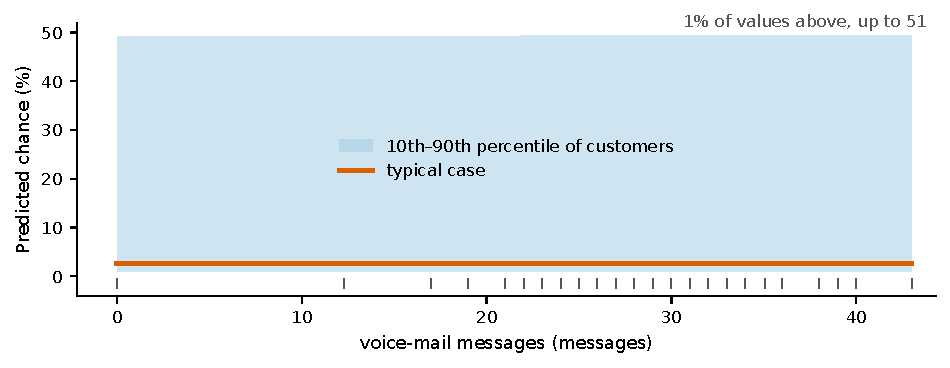
\includegraphics[width=\linewidth,height=0.88\textheight,keepaspectratio]{figures/churn100-s4-c2/ann_84-response.pdf}
\caption{Small voice-mail unit: Response curves through this part: the typical case (bold), the 10th to 90th percentile of individual customers (band), the fold or step point (dashed) with its spread across them (grey), and the observed values (ticks).}
\label{fig:churn100s4c2:plot-ann84-0}
\end{figure}
\begin{figure}[H]\centering
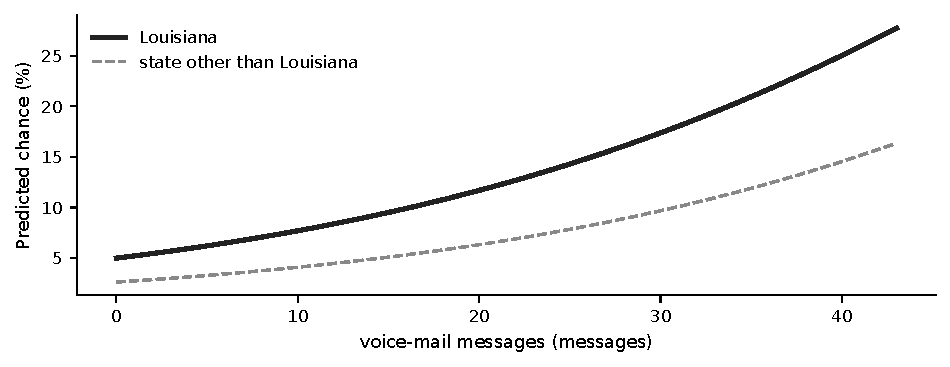
\includegraphics[width=\linewidth,height=0.88\textheight,keepaspectratio]{figures/churn100-s4-c2/ann_84-interaction.pdf}
\caption{Small voice-mail unit: How the effect differs between groups: one curve per group, for the typical case of each group.}
\label{fig:churn100s4c2:plot-ann84-1}
\end{figure}
\begin{figure}[H]\centering
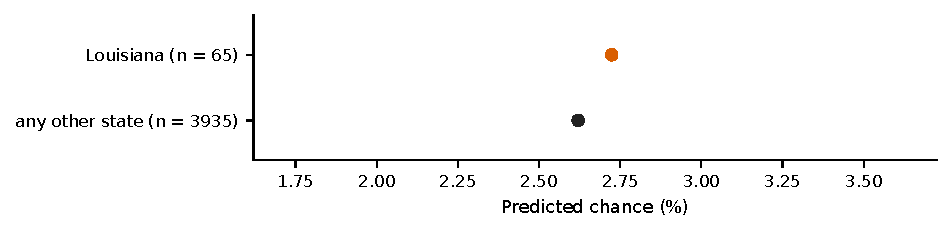
\includegraphics[width=\linewidth,height=0.88\textheight,keepaspectratio]{figures/churn100-s4-c2/ann_84-categories-small.pdf}
\caption{Small voice-mail unit: The predicted value for the typical case at each level, through this part (n = training customers; grey: fewer than 20).}
\label{fig:churn100s4c2:plot-ann84-2}
\end{figure}
\begin{figure}[H]\centering
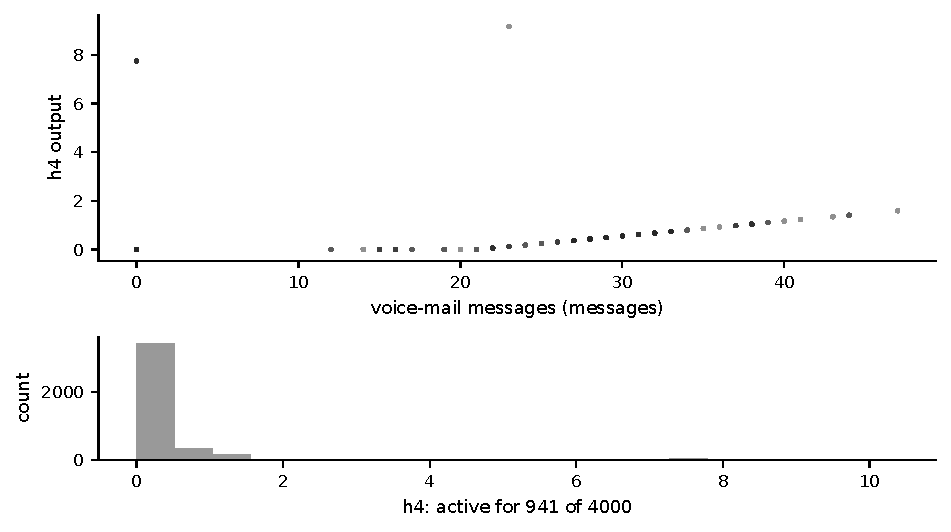
\includegraphics[width=\linewidth,height=0.88\textheight,keepaspectratio]{figures/churn100-s4-c2/ann_84-units.pdf}
\caption{Small voice-mail unit: This part's hidden units: each unit's output against its main numeric input (top) and how often it is active (bottom).}
\label{fig:churn100s4c2:plot-ann84-3}
\end{figure}
\par\smallskip\noindent{\small Technical detail: \ref{tech:ann84}.\par}
\subsection{Not supported by the model}
\begin{itemize}\setlength\itemsep{0pt}\small
\item C109: threshold claim about number of voice-mail messages in part ann\_\allowbreak{}84: not supported by the model (the fold changes the curve by only 0.007 log-odds compared with a straight line (needed 0.1); the effect past the fold is too small or not consistent across patients).
\item C110: subgroup claim about state and number of voice-mail messages in part ann\_\allowbreak{}84: not supported by the model (its effect is negligible).
\item C113: boundary claim about total daytime minutes and number of voice-mail messages in part ann\_\allowbreak{}82: not supported by the model (the boundary rule matches 0.0 of training rows (needs 0.99)).
\end{itemize}
\clearpage\section*{Technical detail: churn100-s4-c2}
\addcontentsline{toc}{section}{Technical detail: churn100-s4-c2}
\noindent{\small The record behind each part: the original hypothesis, the closed form, and every claim with its estimate (log-odds and odds ratio), range across patients, n and test check.\par}
\renewcommand{\thesubsection}{T.\arabic{subsection}}\setcounter{subsection}{0}
\subsection{The whole model}\label{tech:ann87}
\noindent{\footnotesize Annotation ann\_\allowbreak{}87 (churn\_\allowbreak{}logit). Reads: state, account length, area code, international calling plan, voice-mail plan, number of voice-mail messages, total daytime minutes, total daytime calls, total daytime charge, total evening minutes, total evening calls, total evening charge, total night-time minutes, total night-time calls, total night-time charge, total international minutes, total international calls, total international charge, number of calls to customer service.\par}
\paragraph{Original hypothesis (unchanged).} Root: logit P(churn) = -1.30 + linear\_\allowbreak{}backbone (identity\_\allowbreak{}lin) + service\_\allowbreak{}calls (identity\_\allowbreak{}svc) + 1.53*3118 + 1.91*10131 (day\_\allowbreak{}usage\_\allowbreak{}hinges) + 0.20*15524 (evening\_\allowbreak{}hinge) - 1.01*1295 - 1.21*7872 + 0.04*9954 (state\_\allowbreak{}offsets) + 0.005*6089, purely additive in the logit; the sigmoid is the only coupling. 37 inputs are unconnected (international charge and calls, night minutes/\allowbreak{}charge/\allowbreak{}calls,\allowbreak{} evening calls, area codes 408/510 and 29 state indicators) and have zero effect. Train AUC 0.8908, accuracy 0.888. Performance sources (train): all children replaced by least-squares linear fits gives AUC 0.8333 (an L2 logistic regression refit on all 71 inputs gets 0.8433); restoring day\_\allowbreak{}usage\_\allowbreak{}hinges alone gives 0.8707, service\_\allowbreak{}calls alone 0.8659, both 0.8907; evening, state and voicemail units restore nothing. So the gain over linear (+0.058) comes from the day-usage and service-call thresholds, which are complementary. Rare-category switches: state:11 -2.75 logit (73 rows, empirical -1.35); state:46 -1.94 (80 rows, -0.91); state:45 -0.94 (91, -0.85); state:47 +0.90 mean (72 rows, empirical +0.92; direct +1.23, but it switches off 10131 so heavy day users lose up to 2.75); state:31 +0.83 (90, +0.67); state:18 +0.41 (65 rows, empirical -0.48: opposite sign); state:39 -0.25 net (82, -0.93: direct -2.61 almost cancelled by the state units).
\paragraph{Closed form.} Read through its parts (their formulas are in their own sections).
\paragraph{Split inputs.} To annotate the parts, the explanation split these inputs into copies (a refactoring step that does not change what the model computes); the diagrams draw each input once: customer-service calls (2 copies); voice-mail messages (3 copies).
\paragraph{State: every level the model reads.} Whole-model change in the predicted chance for a typical customer when only the state changes from the reference; n = training customers in that level.\par\smallskip
{\scriptsize\rowcolors{2}{black!6}{white}
\begin{longtable}{@{}lllrlc@{}}
\toprule\rowcolor{white}
Claim & From & To & n & Chance & OK \\
\midrule\endhead
\bottomrule\endfoot
C002 & West Virginia & Washington & 72 & 3\% to 11\% & \textcolor{OliveGreen}{yes} \\
C005 & West Virginia & New Jersey & 90 & 3\% to 7\% & \textcolor{OliveGreen}{yes} \\
C008 & West Virginia & Louisiana & 65 & 3\% to 5\% & \textcolor{OliveGreen}{yes} \\
C009 & West Virginia & Connecticut & 80 & 3\% to 5\% & \textcolor{OliveGreen}{yes} \\
C013 & West Virginia & Tennessee & 68 & 3\% to 5\% & \textcolor{OliveGreen}{yes} \\
C014 & West Virginia & Massachusetts & 86 & 3\% to 5\% & \textcolor{OliveGreen}{yes} \\
C015 & West Virginia & Oregon & 84 & 3\% to 4\% & \textcolor{OliveGreen}{yes} \\
C016 & West Virginia & Indiana & 82 & 3\% to 4\% & \textcolor{OliveGreen}{yes} \\
C017 & West Virginia & Kentucky & 81 & 3\% to 4\% & \textcolor{OliveGreen}{yes} \\
C019 & West Virginia & South Dakota & 66 & 3\% to 4\% & \textcolor{OliveGreen}{yes} \\
C020 & West Virginia & Oklahoma & 79 & 3\% to 4\% & \textcolor{OliveGreen}{yes} \\
C024 & West Virginia & North Dakota & 68 & 3\% to 3\% & \textcolor{OliveGreen}{yes} \\
C025 & West Virginia & state other than Georgia, Hawaii, Indiana, Kentucky, Loui... & 2286 & 3\% to 3\% & \textcolor{OliveGreen}{yes} \\
C027 & West Virginia & Arizona & 73 & 3\% to 3\% & \textcolor{OliveGreen}{yes} \\
C030 & West Virginia & Arkansas & 78 & 3\% to 3\% & \textcolor{OliveGreen}{yes} \\
C033 & West Virginia & Rhode Island & 82 & 3\% to 3\% & \textcolor{OliveGreen}{yes} \\
C034 & West Virginia & Florida & 78 & 3\% to 3\% & \textcolor{OliveGreen}{yes} \\
C023 & West Virginia & Pennsylvania & 56 & 3\% to 2\% & \textcolor{OliveGreen}{yes} \\
C022 & West Virginia & Georgia & 60 & 3\% to 2\% & \textcolor{OliveGreen}{yes} \\
C018 & West Virginia & Virginia & 91 & 3\% to 1\% & \textcolor{OliveGreen}{yes} \\
C012 & West Virginia & Vermont & 80 & 3\% to $<$1\% & \textcolor{OliveGreen}{yes} \\
C007 & West Virginia & Hawaii & 73 & 3\% to $<$1\% & \textcolor{OliveGreen}{yes} \\
\end{longtable}}
\paragraph{Evidence table} (next page, landscape).
\begin{landscape}
{\scriptsize\setlength{\tabcolsep}{3pt}\renewcommand{\arraystretch}{1.15}
\rowcolors{2}{black!6}{white}
\begin{longtable}{@{}l>{\raggedright\arraybackslash}p{0.36\linewidth}>{\raggedright\arraybackslash}p{0.14\linewidth}rrr>{\raggedright\arraybackslash}p{0.06\linewidth}>{\raggedright\arraybackslash}p{0.17\linewidth}c@{}}
\toprule\rowcolor{white}
ID & What is checked & Risk, typical patient & Log-odds & OR & Range (p10--p90) & n & Test check & OK \\
\midrule\endfirsthead
\toprule\rowcolor{white}
ID & What is checked & Risk, typical patient & Log-odds & OR & Range (p10--p90) & n & Test check & OK \\
\midrule\endhead
\bottomrule\endfoot
C001 & direction: international calling plan: no international plan to an international plan (whole model) \newline{\itshape shape: categorical; highest to lowest: an international plan, no international plan} & 3\% to 31\% & 2.82 & 16.7 & 2.82 to 2.82 & 3620, 380 & agrees; AUC gain 0.060 [0.032, 0.090] & \textcolor{OliveGreen}{yes} \\
C002 & direction: state: West Virginia to Washington (whole model) \newline{\itshape shape: categorical; highest to lowest: Washington, New Jersey, Louisiana, Connecticut, Tennessee, Massachusetts ...} & 3\% to 11\% & 1.27 & 3.58 & 0.64 to 1.48 & 122, 72 & disagrees; AUC gain -0.012 [-0.026, 0.0005] & \textcolor{OliveGreen}{yes} \\
C003 & direction: voice-mail messages: 0 messages to 32 messages (whole model) \newline{\itshape shape: steady; 72\% of patients same; fallback; risk saturates near 0\%} & 3\% to 11\% & 1.21 & 3.35 & 0.39 to 1.47 & 4000 & agrees; AUC gain 0.017 [0.005, 0.031] & \textcolor{OliveGreen}{yes} \\
C004 & direction: total daytime minutes: 112 minutes to 249 minutes (whole model) \newline{\itshape shape: hinge at 223 minutes; 50\% of patients same; fallback; risk saturates near 0\%; matches the fold at 221 minutes} & 3\% to 8\% & 1.13 & 3.10 & 0.83 to 1.79 & 4000 & agrees; AUC gain 0.036 [0.015, 0.059] & \textcolor{OliveGreen}{yes} \\
C005 & direction: state: West Virginia to New Jersey (whole model) \newline{\itshape shape: categorical; highest to lowest: Washington, New Jersey, Louisiana, Connecticut, Tennessee, Massachusetts ...} & 3\% to 7\% & 1.09 & 2.97 & 1.09 to 1.09 & 122, 90 & disagrees; AUC gain -0.012 [-0.026, 0.0005] & \textcolor{OliveGreen}{yes} \\
C006 & direction: voice-mail plan: no voice-mail plan to a voice-mail plan (whole model) \newline{\itshape shape: categorical; highest to lowest: no voice-mail plan, a voice-mail plan} & 3\% to $<$1\% & -2.54 & 0.08 & -2.54 to -2.54 & 2939, 1061 & agrees; AUC gain 0.033 [0.014, 0.053] & \textcolor{OliveGreen}{yes} \\
C007 & direction: state: West Virginia to Hawaii (whole model) \newline{\itshape shape: categorical; highest to lowest: Washington, New Jersey, Louisiana, Connecticut, Tennessee, Massachusetts ...} & 3\% to $<$1\% & -2.50 & 0.08 & -2.50 to -2.50 & 122, 73 & disagrees; AUC gain -0.012 [-0.026, 0.0005] & \textcolor{OliveGreen}{yes} \\
C008 & direction: state: West Virginia to Louisiana (whole model) \newline{\itshape shape: categorical; highest to lowest: Washington, New Jersey, Louisiana, Connecticut, Tennessee, Massachusetts ...} & 3\% to 5\% & 0.67 & 1.95 & 0.67 to 0.67 & 122, 65 & disagrees; AUC gain -0.012 [-0.026, 0.0005] & \textcolor{OliveGreen}{yes} \\
C009 & direction: state: West Virginia to Connecticut (whole model) \newline{\itshape shape: categorical; highest to lowest: Washington, New Jersey, Louisiana, Connecticut, Tennessee, Massachusetts ...} & 3\% to 5\% & 0.66 & 1.94 & 0.66 to 0.66 & 122, 80 & disagrees; AUC gain -0.012 [-0.026, 0.0005] & \textcolor{OliveGreen}{yes} \\
C010 & direction: total evening charge: 11.76 US dollars to 22.57 US dollars (whole model) \newline{\itshape shape: steady; 100\% of patients same; verified; risk saturates near 0\%} & 2\% to 4\% & 0.88 & 2.42 & 0.88 to 0.88 & 4000 & agrees; AUC gain 0.013 [0.004, 0.022] & \textcolor{OliveGreen}{yes} \\
C011 & direction: total international minutes: 7 minutes to 14 minutes (whole model) \newline{\itshape shape: steady; 100\% of patients same; verified; risk saturates near 0\%} & 2\% to 4\% & 0.85 & 2.35 & 0.85 to 0.85 & 4000 & unclear; AUC gain 0.0008 [-0.007, 0.008] & \textcolor{OliveGreen}{yes} \\
C012 & direction: state: West Virginia to Vermont (whole model) \newline{\itshape shape: categorical; highest to lowest: Washington, New Jersey, Louisiana, Connecticut, Tennessee, Massachusetts ...} & 3\% to $<$1\% & -1.68 & 0.19 & -1.68 to -1.68 & 122, 80 & disagrees; AUC gain -0.012 [-0.026, 0.0005] & \textcolor{OliveGreen}{yes} \\
C013 & direction: state: West Virginia to Tennessee (whole model) \newline{\itshape shape: categorical; highest to lowest: Washington, New Jersey, Louisiana, Connecticut, Tennessee, Massachusetts ...} & 3\% to 5\% & 0.60 & 1.82 & 0.60 to 0.60 & 122, 68 & disagrees; AUC gain -0.012 [-0.026, 0.0005] & \textcolor{OliveGreen}{yes} \\
C014 & direction: state: West Virginia to Massachusetts (whole model) \newline{\itshape shape: categorical; highest to lowest: Washington, New Jersey, Louisiana, Connecticut, Tennessee, Massachusetts ...} & 3\% to 5\% & 0.57 & 1.77 & 0.57 to 0.57 & 122, 86 & disagrees; AUC gain -0.012 [-0.026, 0.0005] & \textcolor{OliveGreen}{yes} \\
C015 & direction: state: West Virginia to Oregon (whole model) \newline{\itshape shape: categorical; highest to lowest: Washington, New Jersey, Louisiana, Connecticut, Tennessee, Massachusetts ...} & 3\% to 4\% & 0.53 & 1.70 & 0.53 to 0.53 & 122, 84 & disagrees; AUC gain -0.012 [-0.026, 0.0005] & \textcolor{OliveGreen}{yes} \\
C016 & direction: state: West Virginia to Indiana (whole model) \newline{\itshape shape: categorical; highest to lowest: Washington, New Jersey, Louisiana, Connecticut, Tennessee, Massachusetts ...} & 3\% to 4\% & 0.52 & 1.69 & 0.52 to 0.52 & 122, 82 & disagrees; AUC gain -0.012 [-0.026, 0.0005] & \textcolor{OliveGreen}{yes} \\
C017 & direction: state: West Virginia to Kentucky (whole model) \newline{\itshape shape: categorical; highest to lowest: Washington, New Jersey, Louisiana, Connecticut, Tennessee, Massachusetts ...} & 3\% to 4\% & 0.47 & 1.61 & 0.47 to 0.47 & 122, 81 & disagrees; AUC gain -0.012 [-0.026, 0.0005] & \textcolor{OliveGreen}{yes} \\
C018 & direction: state: West Virginia to Virginia (whole model) \newline{\itshape shape: categorical; highest to lowest: Washington, New Jersey, Louisiana, Connecticut, Tennessee, Massachusetts ...} & 3\% to 1\% & -0.69 & 0.50 & -0.69 to -0.69 & 122, 91 & disagrees; AUC gain -0.012 [-0.026, 0.0005] & \textcolor{OliveGreen}{yes} \\
C019 & direction: state: West Virginia to South Dakota (whole model) \newline{\itshape shape: categorical; highest to lowest: Washington, New Jersey, Louisiana, Connecticut, Tennessee, Massachusetts ...} & 3\% to 4\% & 0.32 & 1.37 & 0.32 to 0.32 & 122, 66 & disagrees; AUC gain -0.012 [-0.026, 0.0005] & \textcolor{OliveGreen}{yes} \\
C020 & direction: state: West Virginia to Oklahoma (whole model) \newline{\itshape shape: categorical; highest to lowest: Washington, New Jersey, Louisiana, Connecticut, Tennessee, Massachusetts ...} & 3\% to 4\% & 0.31 & 1.36 & 0.31 to 0.31 & 122, 79 & disagrees; AUC gain -0.012 [-0.026, 0.0005] & \textcolor{OliveGreen}{yes} \\
C021 & direction: total daytime calls: 75 calls to 125 calls (whole model) \newline{\itshape shape: steady; 100\% of patients same; verified; risk saturates near 0\%} & 2\% to 3\% & 0.33 & 1.40 & 0.33 to 0.33 & 4000 & disagrees; AUC gain -0.002 [-0.005, 0.0008] & \textcolor{OliveGreen}{yes} \\
C022 & direction: state: West Virginia to Georgia (whole model) \newline{\itshape shape: categorical; highest to lowest: Washington, New Jersey, Louisiana, Connecticut, Tennessee, Massachusetts ...} & 3\% to 2\% & -0.40 & 0.67 & -0.40 to -0.40 & 122, 60 & disagrees; AUC gain -0.012 [-0.026, 0.0005] & \textcolor{OliveGreen}{yes} \\
C023 & direction: state: West Virginia to Pennsylvania (whole model) \newline{\itshape shape: categorical; highest to lowest: Washington, New Jersey, Louisiana, Connecticut, Tennessee, Massachusetts ...} & 3\% to 2\% & -0.37 & 0.69 & -0.37 to -0.37 & 122, 56 & disagrees; AUC gain -0.012 [-0.026, 0.0005] & \textcolor{OliveGreen}{yes} \\
C024 & direction: state: West Virginia to North Dakota (whole model) \newline{\itshape shape: categorical; highest to lowest: Washington, New Jersey, Louisiana, Connecticut, Tennessee, Massachusetts ...} & 3\% to 3\% & 0.26 & 1.30 & 0.26 to 0.26 & 122, 68 & disagrees; AUC gain -0.012 [-0.026, 0.0005] & \textcolor{OliveGreen}{yes} \\
C025 & direction: state: West Virginia to state other than Georgia, Hawaii, Indiana, Kentucky, Louisiana, Massachusetts, Arkansas, North Dakota, Arizona, New Jersey, Oklahoma, Oregon, Pennsylvania, Rhode Island, South Dakota, Tennessee, Virginia, Vermont, Washington, West Virginia, Connecticut, Florida (whole model) \newline{\itshape shape: categorical; highest to lowest: Washington, New Jersey, Louisiana, Connecticut, Tennessee, Massachusetts ...} & 3\% to 3\% & 0.26 & 1.29 & 0.26 to 0.26 & 122, 2286 & disagrees; AUC gain -0.012 [-0.026, 0.0005] & \textcolor{OliveGreen}{yes} \\
C026 & direction: account length: 48 to 152 (whole model) \newline{\itshape shape: steady; 100\% of patients same; verified; risk saturates near 0\%} & 2\% to 3\% & 0.28 & 1.32 & 0.28 to 0.28 & 4000 & disagrees; AUC gain -0.001 [-0.004, 0.0006] & \textcolor{OliveGreen}{yes} \\
C027 & direction: state: West Virginia to Arizona (whole model) \newline{\itshape shape: categorical; highest to lowest: Washington, New Jersey, Louisiana, Connecticut, Tennessee, Massachusetts ...} & 3\% to 3\% & 0.22 & 1.25 & 0.22 to 0.22 & 122, 73 & disagrees; AUC gain -0.012 [-0.026, 0.0005] & \textcolor{OliveGreen}{yes} \\
C028 & direction: total evening minutes: 138 minutes to 266 minutes (whole model) \newline{\itshape shape: hinge at 218 minutes; 100\% of patients same; verified; risk saturates near 0\%; matches the fold at 217 minutes} & 3\% to 3\% & 0.20 & 1.22 & 0.20 to 0.20 & 4000 & unclear; AUC gain 0.003 [-8e-05, 0.005] & \textcolor{OliveGreen}{yes} \\
C029 & direction: customer-service calls: 0 calls to 3 calls (whole model) \newline{\itshape shape: accelerating; 100\% of patients same; verified; risk saturates near 0\%} & 3\% to 3\% & 0.19 & 1.21 & 0.19 to 0.19 & 4000 & agrees; AUC gain 0.111 [0.070, 0.152] & \textcolor{OliveGreen}{yes} \\
C030 & direction: state: West Virginia to Arkansas (whole model) \newline{\itshape shape: categorical; highest to lowest: Washington, New Jersey, Louisiana, Connecticut, Tennessee, Massachusetts ...} & 3\% to 3\% & 0.14 & 1.15 & 0.14 to 0.14 & 122, 78 & disagrees; AUC gain -0.012 [-0.026, 0.0005] & \textcolor{OliveGreen}{yes} \\
C031 & direction: area code: area code 415 to area code other than area code 415 (whole model) \newline{\itshape shape: categorical; highest to lowest: area code 415, area code other than area code 415} & 3\% to 3\% & -0.01 & 0.99 & -0.01 to -0.01 & 2016, 1984 & disagrees; AUC gain -0.0002 [-0.0004, 5e-05] & \textcolor{OliveGreen}{yes} \\
C032 & direction: total daytime charge: 19.07 US dollars to 42.40 US dollars (whole model) \newline{\itshape shape: hinge at 42.20 US dollars; 77\% of patients same; fallback; risk saturates near 0\%; matches the fold at 39.34 US dollars} & 3\% to 3\% & 0.24 & 1.27 & 0.00 to 0.94 & 4000 & unclear; AUC gain 0.005 [-0.0004, 0.012] & \textcolor{OliveGreen}{yes} \\
C033 & direction: state: West Virginia to Rhode Island (whole model) \newline{\itshape shape: categorical; highest to lowest: Washington, New Jersey, Louisiana, Connecticut, Tennessee, Massachusetts ...} & 3\% to 3\% & 0.004 & 1.00 & 0.004 to 0.004 & 122, 82 & disagrees; AUC gain -0.012 [-0.026, 0.0005] & \textcolor{OliveGreen}{yes} \\
C034 & direction: state: West Virginia to Florida (whole model) \newline{\itshape shape: categorical; highest to lowest: Washington, New Jersey, Louisiana, Connecticut, Tennessee, Massachusetts ...} & 3\% to 3\% & -0.0006 & 1.00 & -0.0006 to -0.0006 & 122, 78 & disagrees; AUC gain -0.012 [-0.026, 0.0005] & \textcolor{OliveGreen}{yes} \\
C035 & magnitude: international calling plan: no international plan to an international plan, typical patient \newline{\itshape shape: categorical; highest to lowest: an international plan, no international plan} & 3\% to 31\% & 2.82 & 16.7 &  & 3620, 380 & agrees; AUC gain 0.060 [0.032, 0.090] & \textcolor{OliveGreen}{yes} \\
C036 & magnitude: state: West Virginia to Washington, typical patient \newline{\itshape shape: categorical; highest to lowest: Washington, New Jersey, Louisiana, Connecticut, Tennessee, Massachusetts ...} & 3\% to 11\% & 1.48 & 4.40 &  & 122, 72 & disagrees; AUC gain -0.012 [-0.026, 0.0005] & \textcolor{OliveGreen}{yes} \\
C037 & magnitude: voice-mail messages: 0 messages to 32 messages, typical patient \newline{\itshape shape: steady; 72\% of patients same; fallback; risk saturates near 0\%} & 3\% to 11\% & 1.47 & 4.37 &  & 4000 & agrees; AUC gain 0.017 [0.005, 0.031] & \textcolor{OliveGreen}{yes} \\
C038 & magnitude: total daytime minutes: 112 minutes to 249 minutes, typical patient \newline{\itshape shape: hinge at 223 minutes; 50\% of patients same; fallback; risk saturates near 0\%; matches the fold at 221 minutes} & 3\% to 8\% & 1.15 & 3.17 &  & 4000 & agrees; AUC gain 0.036 [0.015, 0.059] & \textcolor{OliveGreen}{yes} \\
C039 & magnitude: voice-mail plan: no voice-mail plan to a voice-mail plan, typical patient \newline{\itshape shape: categorical; highest to lowest: no voice-mail plan, a voice-mail plan} & 3\% to $<$1\% & -2.54 & 0.08 &  & 2939, 1061 & agrees; AUC gain 0.033 [0.014, 0.053] & \textcolor{OliveGreen}{yes} \\
C040 & null: model ignores total evening calls (exact rule) &  & 0.00 &  &  & 4000 & train only & \textcolor{OliveGreen}{yes} \\
C041 & null: model ignores total international calls (exact rule) &  & 0.00 &  &  & 4000 & train only & \textcolor{OliveGreen}{yes} \\
C042 & null: model ignores total international charge (exact rule) &  & 0.00 &  &  & 4000 & train only & \textcolor{OliveGreen}{yes} \\
C043 & null: model ignores total night-time calls (exact rule) &  & 0.00 &  &  & 4000 & train only & \textcolor{OliveGreen}{yes} \\
C044 & null: model ignores total night-time charge (exact rule) &  & 0.00 &  &  & 4000 & train only & \textcolor{OliveGreen}{yes} \\
C045 & null: model ignores total night-time minutes (exact rule) &  & 0.00 &  &  & 4000 & train only & \textcolor{OliveGreen}{yes} \\
C046 & structure: made of linear\_\allowbreak{}backbone, service\_\allowbreak{}calls, day\_\allowbreak{}usage\_\allowbreak{}hinges, evening\_\allowbreak{}hinge, vmail\_\allowbreak{}state18\_\allowbreak{}unit, state\_\allowbreak{}offsets; added &  &  &  &  & 4000 & train only & \textcolor{OliveGreen}{yes} \\
\end{longtable}}
\end{landscape}
\subsection{Fixed-weight inputs}\label{tech:ann79}
\noindent{\footnotesize Annotation ann\_\allowbreak{}79 (linear\_\allowbreak{}backbone). Reads: state, account length, area code, international calling plan, voice-mail plan, number of voice-mail messages, total daytime calls, total evening charge, total international minutes.\par}
\paragraph{Original hypothesis (unchanged).} Direct input-to-output edges collected through identity\_\allowbreak{}lin (an identity node). Exactly linear in 29 inputs: voicemail plan -1.12 per SD (-2.54 logit for having a plan, mostly offset for heavy message users by voicemail messages +0.62 per SD), international plan +0.83 (+2.82 logit for having one), evening charge +0.35, international minutes +0.34, day calls +0.13, account length +0.11, and state offsets: state:11 -0.37 (-2.75 logit for its 73 customers), state:39 -0.37 (-2.61, but the state\_\allowbreak{}offsets units give back +2.36), state:46 -0.27 (-1.94), state:47 +0.16 (+1.23), state:31 +0.12 (+0.83), state:45 -0.14 (-0.94), then smaller states and area code 415 (+0.01). Day minutes, day charge and customer-service calls have NO direct edge: they act only through hinges. Evidence: closed form exact (identity); train sensitivities equal the weights (voicemail plan 1.12, voicemail messages 0.62, international plan 0.83).
\paragraph{Closed form} {\footnotesize(weights and biases at 3 significant figures; largest difference from the part on the training patients 1.33227e-15).}
{\small\begingroup\allowdisplaybreaks
\begin{align*}
y_{0} &= 0.00719 x_{areaCode:415} + 0.106 x_{accountLength} + 0.0569 x_{state:6} \\
&\qquad + 0.163 x_{state:47\_a} + 0.133 x_{totalDayCalls} + 0.337 x_{totalIntlMinutes} \\
&\qquad + 0.044 x_{state:42} + 0.007 x_{state:36} + 0.00781 x_{state:41} \\
&\qquad + 0.621 x_{numberVmailMessages\_a} + 0.0397 x_{state:37} + 0.35 x_{totalEveCharge} \\
&\qquad + 0.0453 x_{state:19} + 0.047 x_{state:18\_a} + 0.826 x_{internationalPlan} \\
&\qquad + 0.000897 x_{state:28} + 0.0307 x_{state:17} + 0.124 x_{state:31} - 0.37 x_{state:39\_a} \\
&\qquad - 0.0355 x_{state:9} - 0.0158 x_{state:2} - 0.00422 x_{state:3} - 0.271 x_{state:46} \\
&\qquad - 1.12 x_{voiceMailPlan} - 0.141 x_{state:45} - 0.044 x_{state:49} - 0.0737 x_{state:38} \\
&\qquad - 0.0797 x_{state:10} - 0.368 x_{state:11}
\end{align*}\endgroup}

\paragraph{Evidence table} (next page, landscape).
\begin{landscape}
{\scriptsize\setlength{\tabcolsep}{3pt}\renewcommand{\arraystretch}{1.15}
\rowcolors{2}{black!6}{white}
\begin{longtable}{@{}l>{\raggedright\arraybackslash}p{0.36\linewidth}>{\raggedright\arraybackslash}p{0.14\linewidth}rrr>{\raggedright\arraybackslash}p{0.06\linewidth}>{\raggedright\arraybackslash}p{0.17\linewidth}c@{}}
\toprule\rowcolor{white}
ID & What is checked & Risk, typical patient & Log-odds & OR & Range (p10--p90) & n & Test check & OK \\
\midrule\endfirsthead
\toprule\rowcolor{white}
ID & What is checked & Risk, typical patient & Log-odds & OR & Range (p10--p90) & n & Test check & OK \\
\midrule\endhead
\bottomrule\endfoot
C047 & direction: international calling plan: no international plan to an international plan (through this part) \newline{\itshape shape: categorical; highest to lowest: an international plan, no international plan} & 3\% to 31\% & 2.82 & 16.7 & 2.82 to 2.82 & 3620, 380 & agrees; AUC gain 0.060 [0.032, 0.090] & \textcolor{OliveGreen}{yes} \\
C048 & direction: state: West Virginia to Washington (through this part) \newline{\itshape shape: categorical; highest to lowest: Washington, New Jersey, Connecticut, Louisiana, Tennessee, Massachusetts ...} & 3\% to 11\% & 1.48 & 4.40 & 1.48 to 1.48 & 122, 72 & disagrees; AUC gain -0.008 [-0.022, 0.005] & \textcolor{OliveGreen}{yes} \\
C049 & direction: voice-mail messages: 0 messages to 32 messages (through this part) \newline{\itshape shape: steady; 100\% of patients same; verified; risk saturates near 0\%} & 3\% to 10\% & 1.47 & 4.35 & 1.47 to 1.47 & 4000 & agrees; AUC gain 0.016 [0.003, 0.029] & \textcolor{OliveGreen}{yes} \\
C050 & direction: state: West Virginia to New Jersey (through this part) \newline{\itshape shape: categorical; highest to lowest: Washington, New Jersey, Connecticut, Louisiana, Tennessee, Massachusetts ...} & 3\% to 7\% & 1.09 & 2.97 & 1.09 to 1.09 & 122, 90 & disagrees; AUC gain -0.008 [-0.022, 0.005] & \textcolor{OliveGreen}{yes} \\
C051 & direction: voice-mail plan: no voice-mail plan to a voice-mail plan (through this part) \newline{\itshape shape: categorical; highest to lowest: no voice-mail plan, a voice-mail plan} & 3\% to $<$1\% & -2.54 & 0.08 & -2.54 to -2.54 & 2939, 1061 & agrees; AUC gain 0.033 [0.014, 0.053] & \textcolor{OliveGreen}{yes} \\
C052 & direction: state: West Virginia to Hawaii (through this part) \newline{\itshape shape: categorical; highest to lowest: Washington, New Jersey, Connecticut, Louisiana, Tennessee, Massachusetts ...} & 3\% to $<$1\% & -2.50 & 0.08 & -2.50 to -2.50 & 122, 73 & disagrees; AUC gain -0.008 [-0.022, 0.005] & \textcolor{OliveGreen}{yes} \\
C053 & direction: state: West Virginia to Rhode Island (through this part) \newline{\itshape shape: categorical; highest to lowest: Washington, New Jersey, Connecticut, Louisiana, Tennessee, Massachusetts ...} & 3\% to $<$1\% & -2.36 & 0.09 & -2.36 to -2.36 & 122, 82 & disagrees; AUC gain -0.008 [-0.022, 0.005] & \textcolor{OliveGreen}{yes} \\
C054 & direction: state: West Virginia to Connecticut (through this part) \newline{\itshape shape: categorical; highest to lowest: Washington, New Jersey, Connecticut, Louisiana, Tennessee, Massachusetts ...} & 3\% to 5\% & 0.66 & 1.94 & 0.66 to 0.66 & 122, 80 & disagrees; AUC gain -0.008 [-0.022, 0.005] & \textcolor{OliveGreen}{yes} \\
C055 & direction: total evening charge: 11.76 US dollars to 22.57 US dollars (through this part) \newline{\itshape shape: steady; 100\% of patients same; verified; risk saturates near 0\%} & 2\% to 4\% & 0.88 & 2.42 & 0.88 to 0.88 & 4000 & agrees; AUC gain 0.013 [0.004, 0.022] & \textcolor{OliveGreen}{yes} \\
C056 & direction: total international minutes: 7 minutes to 14 minutes (through this part) \newline{\itshape shape: steady; 100\% of patients same; verified; risk saturates near 0\%} & 2\% to 4\% & 0.85 & 2.35 & 0.85 to 0.85 & 4000 & unclear; AUC gain 0.0008 [-0.007, 0.008] & \textcolor{OliveGreen}{yes} \\
C057 & direction: state: West Virginia to Louisiana (through this part) \newline{\itshape shape: categorical; highest to lowest: Washington, New Jersey, Connecticut, Louisiana, Tennessee, Massachusetts ...} & 3\% to 5\% & 0.63 & 1.87 & 0.63 to 0.63 & 122, 65 & disagrees; AUC gain -0.008 [-0.022, 0.005] & \textcolor{OliveGreen}{yes} \\
C058 & direction: state: West Virginia to Vermont (through this part) \newline{\itshape shape: categorical; highest to lowest: Washington, New Jersey, Connecticut, Louisiana, Tennessee, Massachusetts ...} & 3\% to $<$1\% & -1.68 & 0.19 & -1.68 to -1.68 & 122, 80 & disagrees; AUC gain -0.008 [-0.022, 0.005] & \textcolor{OliveGreen}{yes} \\
C059 & direction: state: West Virginia to Tennessee (through this part) \newline{\itshape shape: categorical; highest to lowest: Washington, New Jersey, Connecticut, Louisiana, Tennessee, Massachusetts ...} & 3\% to 5\% & 0.60 & 1.82 & 0.60 to 0.60 & 122, 68 & disagrees; AUC gain -0.008 [-0.022, 0.005] & \textcolor{OliveGreen}{yes} \\
C060 & direction: state: West Virginia to Massachusetts (through this part) \newline{\itshape shape: categorical; highest to lowest: Washington, New Jersey, Connecticut, Louisiana, Tennessee, Massachusetts ...} & 3\% to 5\% & 0.57 & 1.77 & 0.57 to 0.57 & 122, 86 & disagrees; AUC gain -0.008 [-0.022, 0.005] & \textcolor{OliveGreen}{yes} \\
C061 & direction: state: West Virginia to Oregon (through this part) \newline{\itshape shape: categorical; highest to lowest: Washington, New Jersey, Connecticut, Louisiana, Tennessee, Massachusetts ...} & 3\% to 4\% & 0.53 & 1.70 & 0.53 to 0.53 & 122, 84 & disagrees; AUC gain -0.008 [-0.022, 0.005] & \textcolor{OliveGreen}{yes} \\
C062 & direction: state: West Virginia to Kentucky (through this part) \newline{\itshape shape: categorical; highest to lowest: Washington, New Jersey, Connecticut, Louisiana, Tennessee, Massachusetts ...} & 3\% to 4\% & 0.47 & 1.61 & 0.47 to 0.47 & 122, 81 & disagrees; AUC gain -0.008 [-0.022, 0.005] & \textcolor{OliveGreen}{yes} \\
C063 & direction: state: West Virginia to Virginia (through this part) \newline{\itshape shape: categorical; highest to lowest: Washington, New Jersey, Connecticut, Louisiana, Tennessee, Massachusetts ...} & 3\% to 1\% & -0.69 & 0.50 & -0.69 to -0.69 & 122, 91 & disagrees; AUC gain -0.008 [-0.022, 0.005] & \textcolor{OliveGreen}{yes} \\
C064 & direction: state: West Virginia to South Dakota (through this part) \newline{\itshape shape: categorical; highest to lowest: Washington, New Jersey, Connecticut, Louisiana, Tennessee, Massachusetts ...} & 3\% to 4\% & 0.32 & 1.37 & 0.32 to 0.32 & 122, 66 & disagrees; AUC gain -0.008 [-0.022, 0.005] & \textcolor{OliveGreen}{yes} \\
C065 & direction: state: West Virginia to Oklahoma (through this part) \newline{\itshape shape: categorical; highest to lowest: Washington, New Jersey, Connecticut, Louisiana, Tennessee, Massachusetts ...} & 3\% to 4\% & 0.31 & 1.36 & 0.31 to 0.31 & 122, 79 & disagrees; AUC gain -0.008 [-0.022, 0.005] & \textcolor{OliveGreen}{yes} \\
C066 & direction: total daytime calls: 75 calls to 125 calls (through this part) \newline{\itshape shape: steady; 100\% of patients same; verified; risk saturates near 0\%} & 2\% to 3\% & 0.33 & 1.40 & 0.33 to 0.33 & 4000 & disagrees; AUC gain -0.002 [-0.005, 0.0008] & \textcolor{OliveGreen}{yes} \\
C067 & direction: state: West Virginia to Georgia (through this part) \newline{\itshape shape: categorical; highest to lowest: Washington, New Jersey, Connecticut, Louisiana, Tennessee, Massachusetts ...} & 3\% to 2\% & -0.40 & 0.67 & -0.40 to -0.40 & 122, 60 & disagrees; AUC gain -0.008 [-0.022, 0.005] & \textcolor{OliveGreen}{yes} \\
C068 & direction: state: West Virginia to Pennsylvania (through this part) \newline{\itshape shape: categorical; highest to lowest: Washington, New Jersey, Connecticut, Louisiana, Tennessee, Massachusetts ...} & 3\% to 2\% & -0.37 & 0.69 & -0.37 to -0.37 & 122, 56 & disagrees; AUC gain -0.008 [-0.022, 0.005] & \textcolor{OliveGreen}{yes} \\
C069 & direction: state: West Virginia to North Dakota (through this part) \newline{\itshape shape: categorical; highest to lowest: Washington, New Jersey, Connecticut, Louisiana, Tennessee, Massachusetts ...} & 3\% to 3\% & 0.26 & 1.30 & 0.26 to 0.26 & 122, 68 & disagrees; AUC gain -0.008 [-0.022, 0.005] & \textcolor{OliveGreen}{yes} \\
C070 & direction: state: West Virginia to state other than Georgia, Hawaii, Kentucky, Louisiana, Massachusetts, Arkansas, North Dakota, Arizona, New Jersey, Oklahoma, Oregon, Pennsylvania, Rhode Island, South Dakota, Tennessee, Virginia, Vermont, Washington, West Virginia, Connecticut, Florida (through this part) \newline{\itshape shape: categorical; highest to lowest: Washington, New Jersey, Connecticut, Louisiana, Tennessee, Massachusetts ...} & 3\% to 3\% & 0.26 & 1.29 & 0.26 to 0.26 & 122, 2368 & disagrees; AUC gain -0.008 [-0.022, 0.005] & \textcolor{OliveGreen}{yes} \\
C071 & direction: account length: 48 to 152 (through this part) \newline{\itshape shape: steady; 100\% of patients same; verified; risk saturates near 0\%} & 2\% to 3\% & 0.28 & 1.32 & 0.28 to 0.28 & 4000 & disagrees; AUC gain -0.001 [-0.004, 0.0006] & \textcolor{OliveGreen}{yes} \\
C072 & direction: state: West Virginia to Arizona (through this part) \newline{\itshape shape: categorical; highest to lowest: Washington, New Jersey, Connecticut, Louisiana, Tennessee, Massachusetts ...} & 3\% to 3\% & 0.22 & 1.25 & 0.22 to 0.22 & 122, 73 & disagrees; AUC gain -0.008 [-0.022, 0.005] & \textcolor{OliveGreen}{yes} \\
C073 & direction: state: West Virginia to Arkansas (through this part) \newline{\itshape shape: categorical; highest to lowest: Washington, New Jersey, Connecticut, Louisiana, Tennessee, Massachusetts ...} & 3\% to 3\% & 0.14 & 1.15 & 0.14 to 0.14 & 122, 78 & disagrees; AUC gain -0.008 [-0.022, 0.005] & \textcolor{OliveGreen}{yes} \\
C074 & direction: area code: area code 415 to area code other than area code 415 (through this part) \newline{\itshape shape: categorical; highest to lowest: area code 415, area code other than area code 415} & 3\% to 3\% & -0.01 & 0.99 & -0.01 to -0.01 & 2016, 1984 & disagrees; AUC gain -0.0002 [-0.0004, 5e-05] & \textcolor{OliveGreen}{yes} \\
C075 & direction: state: West Virginia to Florida (through this part) \newline{\itshape shape: categorical; highest to lowest: Washington, New Jersey, Connecticut, Louisiana, Tennessee, Massachusetts ...} & 3\% to 3\% & -0.0006 & 1.00 & -0.0006 to -0.0006 & 122, 78 & disagrees; AUC gain -0.008 [-0.022, 0.005] & \textcolor{OliveGreen}{yes} \\
C076 & structure: its formula reproduces it on 4000 training patients (largest difference 1.33227e-15) &  & 1e-15 &  &  & 4000 & train only & \textcolor{OliveGreen}{yes} \\
\end{longtable}}
\end{landscape}
\subsection{Service calls}\label{tech:ann86}
\noindent{\footnotesize Annotation ann\_\allowbreak{}86 (service\_\allowbreak{}calls). Reads: number of calls to customer service.\par}
\paragraph{Original hypothesis (unchanged).} Composition of csc\_\allowbreak{}moderate\_\allowbreak{}chain and csc\_\allowbreak{}high\_\allowbreak{}hinge: their exits are summed by identity\_\allowbreak{}svc = 1.66*5268 + 1.76*9436 + 1.54*6713, which enters the logit with weight 1; they read the same input (two split copies of customer-service calls). Hypothesis: all of the model's service-call effect is a threshold: nothing for 0-2 calls, +0.19 logit at 3 calls, then about +2.4 logit per extra call (+2.07 at 4, +4.44 at 5, +6.81 at 6, +9.18 at 7). Evidence (train): churn by calls 0-7 is 0.115/\allowbreak{}0.110/\allowbreak{}0.110/\allowbreak{}0.106/\allowbreak{}0.437/\allowbreak{}0.571/\allowbreak{}0.679/\allowbreak{}0.545 against model 0.118/\allowbreak{}0.108/\allowbreak{}0.105/\allowbreak{}0.115/\allowbreak{}0.327/\allowbreak{}0.749/\allowbreak{}0.956/\allowbreak{}0.986: the threshold is right, but the model under-predicts at 4 calls and is over-confident from 5 calls (116 customers). Mean-ablating both children gives AUC 0.7976, linear replacement 0.8711; restoring service\_\allowbreak{}calls alone onto the all-linear model gives 0.8659 (all-linear 0.8333).
\paragraph{Closed form.} Read through its parts (their formulas are in their own sections).
\paragraph{Evidence table} (next page, landscape).
\begin{landscape}
{\scriptsize\setlength{\tabcolsep}{3pt}\renewcommand{\arraystretch}{1.15}
\rowcolors{2}{black!6}{white}
\begin{longtable}{@{}l>{\raggedright\arraybackslash}p{0.36\linewidth}>{\raggedright\arraybackslash}p{0.14\linewidth}rrr>{\raggedright\arraybackslash}p{0.06\linewidth}>{\raggedright\arraybackslash}p{0.17\linewidth}c@{}}
\toprule\rowcolor{white}
ID & What is checked & Risk, typical patient & Log-odds & OR & Range (p10--p90) & n & Test check & OK \\
\midrule\endfirsthead
\toprule\rowcolor{white}
ID & What is checked & Risk, typical patient & Log-odds & OR & Range (p10--p90) & n & Test check & OK \\
\midrule\endhead
\bottomrule\endfoot
C077 & direction: customer-service calls: 0 calls to 3 calls (through this part) \newline{\itshape shape: accelerating; 100\% of patients same; verified; risk saturates near 0\%} & 3\% to 3\% & 0.19 & 1.21 & 0.19 to 0.19 & 4000 & agrees; AUC gain 0.111 [0.070, 0.152] & \textcolor{OliveGreen}{yes} \\
C078 & threshold: customer-service calls: fold at about 3 calls (starts) \newline{\itshape shape: accelerating; 100\% of patients same; verified; risk saturates near 0\%} & 3\% to 18\% (typical patient with a fold) & 2.07 & 7.90 & 2.07 to 2.07 & 4000, 848 & agrees; AUC gain 0.111 [0.070, 0.152] & \textcolor{OliveGreen}{yes} \\
C079 & structure: made of csc\_\allowbreak{}moderate\_\allowbreak{}chain, csc\_\allowbreak{}high\_\allowbreak{}hinge; added &  &  &  &  & 4000 & train only & \textcolor{OliveGreen}{yes} \\
\end{longtable}}
\end{landscape}
\subsection{Calls from 4 upwards}\label{tech:ann81}
\noindent{\footnotesize Annotation ann\_\allowbreak{}81 (csc\_\allowbreak{}high\_\allowbreak{}hinge). Reads: number of calls to customer service.\par}
\paragraph{Original hypothesis (unchanged).} 9436 = relu(-0.58 + 0.46 csc), 6713 = relu(-0.13 + 1.43*9436); logit weights +1.76 and +1.54 (via identity\_\allowbreak{}svc). Hypothesis: a second hinge on customer-service calls, off for 0-3 calls and switching on from 4 calls, adding about +1.4 logit per extra call (+0.91 at 4, +2.32 at 5, +3.72 at 6). Active on exactly the 8\% of customers with 4+ calls (318 rows; empirical churn jumps from 0.11 at 3 calls to 0.44 at 4). Evidence: line plot correlation 0.66; mean ablation AUC 0.8761; linear replacement 0.8857 (R2 0.44/0.41); restored alone onto all-linear 0.8571.
\paragraph{Closed form} {\footnotesize(weights and biases at 3 significant figures; largest difference from the part on the training patients 0.0).}
{\small\begingroup\allowdisplaybreaks
\begin{align*}
y_{0} &= \operatorname{relu}\bigl(-0.582 + 0.462 x_{numberCustomerServiceCalls\_b}\bigr) \\
y_{1} &= \operatorname{relu}\bigl(-0.127 + 1.43 \operatorname{relu}\bigl(-0.582 \\
&\qquad + 0.462 x_{numberCustomerServiceCalls\_b}\bigr)\bigr)
\end{align*}\endgroup}

\paragraph{Evidence table} (next page, landscape).
\begin{landscape}
{\scriptsize\setlength{\tabcolsep}{3pt}\renewcommand{\arraystretch}{1.15}
\rowcolors{2}{black!6}{white}
\begin{longtable}{@{}l>{\raggedright\arraybackslash}p{0.36\linewidth}>{\raggedright\arraybackslash}p{0.14\linewidth}rrr>{\raggedright\arraybackslash}p{0.06\linewidth}>{\raggedright\arraybackslash}p{0.17\linewidth}c@{}}
\toprule\rowcolor{white}
ID & What is checked & Risk, typical patient & Log-odds & OR & Range (p10--p90) & n & Test check & OK \\
\midrule\endfirsthead
\toprule\rowcolor{white}
ID & What is checked & Risk, typical patient & Log-odds & OR & Range (p10--p90) & n & Test check & OK \\
\midrule\endhead
\bottomrule\endfoot
C093 & threshold: customer-service calls: fold at about 4 calls (starts) \newline{\itshape shape: accelerating; 100\% of patients same; verified; risk saturates near 0\%} & 3\% to 6\% (typical patient with a fold) & 0.91 & 2.49 & 0.91 to 0.91 & 4000, 318 & agrees; AUC gain 0.023 [0.012, 0.035] & \textcolor{OliveGreen}{yes} \\
C094 & subgroup: who this part acts on: 318 of 4000 patients & 8\% to 18\% (typical patient this part acts on (risk without the part, then with it)) & 1.71 & 5.51 & 0.91 to 3.72 & 318, 3682 & agrees; AUC gain 0.023 [0.012, 0.035] & \textcolor{OliveGreen}{yes} \\
C095 & structure: its formula reproduces it on 4000 training patients (largest difference 0.0) &  & 0.00 &  &  & 4000 & train only & \textcolor{OliveGreen}{yes} \\
\end{longtable}}
\end{landscape}
\subsection{Calls from 3 upwards}\label{tech:ann80}
\noindent{\footnotesize Annotation ann\_\allowbreak{}80 (csc\_\allowbreak{}moderate\_\allowbreak{}chain). Reads: number of calls to customer service.\par}
\paragraph{Original hypothesis (unchanged).} 12730 = relu(-0.03 + 0.80 csc), 12171 = relu(-0.44 + 0.84 csc + 0.72*12730), 5268 = relu(-0.56 + 0.25 csc + 0.36*12171); logit weight +1.66 (via identity\_\allowbreak{}svc). Hypothesis: a convex hinge on customer-service calls that is zero for 0-2 calls, just switches on at 3 calls (mean logit +0.19) and then adds about +1.0 logit per extra call (+1.16 at 4, +2.12 at 5, +3.09 at 6). Evidence (train, n=4000): line plot of 5268 against calls rises from 0 to 3.6 (correlation 0.74); 5268 active on 21\% of customers (all with 3+ calls). Mean ablation AUC 0.8733 (full 0.8908); linear replacement 0.8852 (R2 0.55); restored alone onto the all-linearised model 0.8565 (all-linear 0.8333).
\paragraph{Closed form} {\footnotesize(weights and biases at 3 significant figures; largest difference from the part on the training patients 4.44089e-16).}
{\small\begingroup\allowdisplaybreaks
\begin{align*}
y_{0} &= \operatorname{relu}\bigl(-0.557 + 0.358 \operatorname{relu}\bigl(-0.443 \\
&\qquad + 0.719 \operatorname{relu}\bigl(-0.0259 + 0.801 x_{numberCustomerServiceCalls\_acd}\bigr) \\
&\qquad + 0.845 x_{numberCustomerServiceCalls\_acd}\bigr) \\
&\qquad + 0.254 x_{numberCustomerServiceCalls\_acd}\bigr)
\end{align*}\endgroup}

\paragraph{Evidence table} (next page, landscape).
\begin{landscape}
{\scriptsize\setlength{\tabcolsep}{3pt}\renewcommand{\arraystretch}{1.15}
\rowcolors{2}{black!6}{white}
\begin{longtable}{@{}l>{\raggedright\arraybackslash}p{0.36\linewidth}>{\raggedright\arraybackslash}p{0.14\linewidth}rrr>{\raggedright\arraybackslash}p{0.06\linewidth}>{\raggedright\arraybackslash}p{0.17\linewidth}c@{}}
\toprule\rowcolor{white}
ID & What is checked & Risk, typical patient & Log-odds & OR & Range (p10--p90) & n & Test check & OK \\
\midrule\endfirsthead
\toprule\rowcolor{white}
ID & What is checked & Risk, typical patient & Log-odds & OR & Range (p10--p90) & n & Test check & OK \\
\midrule\endhead
\bottomrule\endfoot
C096 & direction: customer-service calls: 0 calls to 3 calls (through this part) \newline{\itshape shape: accelerating; 100\% of patients same; verified; risk saturates near 0\%} & 3\% to 3\% & 0.19 & 1.21 & 0.19 to 0.19 & 4000 & agrees; AUC gain 0.028 [0.014, 0.042] & \textcolor{OliveGreen}{yes} \\
C097 & threshold: customer-service calls: fold at about 3 calls (starts) \newline{\itshape shape: accelerating; 100\% of patients same; verified; risk saturates near 0\%} & 3\% to 8\% (typical patient with a fold) & 1.16 & 3.18 & 1.16 to 1.16 & 4000, 848 & agrees; AUC gain 0.028 [0.014, 0.042] & \textcolor{OliveGreen}{yes} \\
C098 & subgroup: who this part acts on: 848 of 4000 patients & 3\% to 4\% (typical patient this part acts on (risk without the part, then with it)) & 0.76 & 2.13 & 0.19 to 2.12 & 848, 3152 & agrees; AUC gain 0.028 [0.014, 0.042] & \textcolor{OliveGreen}{yes} \\
C099 & structure: its formula reproduces it on 4000 training patients (largest difference 4.44089e-16) &  & 4e-16 &  &  & 4000 & train only & \textcolor{OliveGreen}{yes} \\
\end{longtable}}
\end{landscape}
\subsection{Heavy daytime use}\label{tech:ann82}
\noindent{\footnotesize Annotation ann\_\allowbreak{}82 (day\_\allowbreak{}usage\_\allowbreak{}hinges). Reads: state, number of voice-mail messages, total daytime minutes, total daytime charge.\par}
\paragraph{Original hypothesis (unchanged).} 3118 = relu(-0.86 + 0.55 dayMin + 0.38 dayCharge - 0.65 vmailMessages), logit weight +1.53; 10131 = relu(-0.72 + 0.84 dayMin - 0.67 state:47), logit weight +1.91. Day minutes and day charge are collinear (r = 1.0000), so 3118 is one hinge in day usage. Hypothesis: day usage has no effect below about 200 minutes, then raises churn risk steeply. 3118 switches on at about 209 day minutes for customers with no voicemail messages (its kink moves up about 25 minutes per 10 messages: 267 at 20, 292 at 30), so it is on for only 2\% of message users; 10131 switches on at about 221 day minutes for everyone except state:47 (off for all 72 state:47 customers). Evidence (train): combined logit contribution 0 below 200 minutes, +0.62 at 220-240, +1.61 at 240-260, +2.59 at 260-280, +4.26 above 280; churn by band 0.06 (200-220), 0.14, 0.26, 0.46, 0.67 vs model 0.08, 0.15, 0.28, 0.43, 0.68 (well calibrated). Sensitivity: 3118 vmail messages 0.15, day minutes 0.12, day charge 0.09; 10131 day minutes 0.18, state:47 0.14. Mean ablation AUC 0.8107 (the largest single drop); linear replacement 0.8657 (R2 0.46/0.45); restored alone onto all-linear 0.8707 (all-linear 0.8333).
\paragraph{Closed form} {\footnotesize(weights and biases at 3 significant figures; largest difference from the part on the training patients 4.44089e-16).}
{\small\begingroup\allowdisplaybreaks
\begin{align*}
y_{0} &= \operatorname{relu}\bigl(-0.856 + 0.382 x_{totalDayCharge} + 0.547 x_{totalDayMinutes} \\
&\qquad - 0.65 x_{numberVmailMessages\_b}\bigr) \\
y_{1} &= \operatorname{relu}\bigl(-0.721 + 0.837 x_{totalDayMinutes} \\
&\qquad - 0.672 x_{state:47\_b}\bigr)
\end{align*}\endgroup}

\paragraph{Evidence table} (next page, landscape).
\begin{landscape}
{\scriptsize\setlength{\tabcolsep}{3pt}\renewcommand{\arraystretch}{1.15}
\rowcolors{2}{black!6}{white}
\begin{longtable}{@{}l>{\raggedright\arraybackslash}p{0.36\linewidth}>{\raggedright\arraybackslash}p{0.14\linewidth}rrr>{\raggedright\arraybackslash}p{0.06\linewidth}>{\raggedright\arraybackslash}p{0.17\linewidth}c@{}}
\toprule\rowcolor{white}
ID & What is checked & Risk, typical patient & Log-odds & OR & Range (p10--p90) & n & Test check & OK \\
\midrule\endfirsthead
\toprule\rowcolor{white}
ID & What is checked & Risk, typical patient & Log-odds & OR & Range (p10--p90) & n & Test check & OK \\
\midrule\endhead
\bottomrule\endfoot
C080 & direction: voice-mail messages: 0 messages to 32 messages (through this part) \newline{\itshape shape: hinge at 11 messages; 64\% of patients same; fallback; one point with C089 (median fold 11 messages, typical patient 11 messages, 10th-90th percentile 4 messages to 27 messages, wide)} & 12\% to 6\% (typical patient this part acts on) & -0.26 & 0.77 & -1.08 to 0.00 & 4000 & agrees; AUC gain 0.006 [0.003, 0.009] & \textcolor{OliveGreen}{yes} \\
C081 & direction: total daytime minutes: 112 minutes to 249 minutes (through this part) \newline{\itshape shape: hinge at 221 minutes; 50\% of patients same; fallback; risk saturates near 0\%; one point with C088 (median fold 221 minutes, typical patient 223 minutes, 10th-90th percentile 186 minutes to 221 minutes, wide)} & 3\% to 8\% & 1.13 & 3.10 & 0.83 to 1.79 & 4000 & agrees; AUC gain 0.036 [0.015, 0.059] & \textcolor{OliveGreen}{yes} \\
C082 & direction: state: state other than Washington to Washington (through this part) \newline{\itshape shape: categorical; highest to lowest: state other than Washington, Washington} & 12\% to 7\% (typical patient this part acts on) & -0.21 & 0.81 & -0.84 to 0.00 & 3928, 72 & agrees; AUC gain 0.0004 [2e-05, 0.0008] & \textcolor{OliveGreen}{yes} \\
C083 & direction: total daytime charge: 19.07 US dollars to 42.40 US dollars (through this part) \newline{\itshape shape: hinge at 39.34 US dollars; 77\% of patients same; fallback; risk saturates near 0\%; one point with C090 (median fold 39.34 US dollars, typical patient 42.20 US dollars, 10th-90th percentile 26.14 US dollars to 52.75 US dollars, wide)} & 3\% to 3\% & 0.24 & 1.27 & 0.00 to 0.94 & 4000 & unclear; AUC gain 0.005 [-0.0004, 0.012] & \textcolor{OliveGreen}{yes} \\
C084 & interaction: effect of total daytime minutes (112 minutes to 249 minutes) by total daytime charge: total daytime charge above 30.69 US dollars minus total daytime charge at or below 30.69 US dollars; stronger in total daytime charge above 30.69 US dollars \newline{\itshape shape: accelerating; 74\% of patients same; fallback; risk saturates near 0\%} & total daytime charge above 30.69 US dollars: 3\% to 11\%; total daytime charge at or below 30.69 US dollars: 3\% to 6\% & 0.54 & 1.71 &  & 1997, 2003 & agrees; AUC gain 0.005 [-0.0004, 0.012] & \textcolor{OliveGreen}{yes} \\
C085 & interaction: effect of total daytime minutes (112 minutes to 249 minutes) by state: Washington minus state other than Washington; stronger in state other than Washington \newline{\itshape shape: hinge at 223 minutes; 51\% of patients same; fallback; risk saturates near 0\%} & Washington: 11\% to 14\%; state other than Washington: 3\% to 8\% & -0.75 & 0.47 &  & 72, 3928 & agrees; AUC gain 0.0004 [2e-05, 0.0008] & \textcolor{OliveGreen}{yes} \\
C086 & interaction: effect of voice-mail messages (0 messages to 32 messages) by total daytime charge: total daytime charge above 30.69 US dollars minus total daytime charge at or below 30.69 US dollars; stronger in total daytime charge at or below 30.69 US dollars \newline{\itshape shape: steady; 100\% of patients same; verified; risk saturates near 0\%} & total daytime charge above 30.69 US dollars: 3\% to 11\%; total daytime charge at or below 30.69 US dollars: 3\% to 11\% & -0.53 & 0.59 &  & 1997, 2003 & agrees; AUC gain 0.005 [-0.0004, 0.012] & \textcolor{OliveGreen}{yes} \\
C087 & interaction: effect of voice-mail messages (0 messages to 32 messages) by total daytime minutes: total daytime minutes above 180 minutes minus total daytime minutes at or below 180 minutes; stronger in total daytime minutes at or below 180 minutes \newline{\itshape shape: steady; 100\% of patients same; verified; risk saturates near 0\%} & total daytime minutes above 180 minutes: 3\% to 11\%; total daytime minutes at or below 180 minutes: 3\% to 11\% & -0.53 & 0.59 &  & 1997, 2003 & agrees; AUC gain 0.036 [0.015, 0.059] & \textcolor{OliveGreen}{yes} \\
C088 & threshold: total daytime minutes: fold at about 221 minutes (starts) \newline{\itshape shape: hinge at 221 minutes; 48\% of patients same; fallback; risk saturates near 0\%; one point with C088 (median fold 221 minutes, typical patient 223 minutes, 10th-90th percentile 186 minutes to 221 minutes, wide)} & 3\% to 19\% (typical patient with a fold) & 1.98 & 7.25 & 1.48 to 2.79 & 3995, 1099 & agrees; AUC gain 0.036 [0.015, 0.059] & \textcolor{OliveGreen}{yes} \\
C089 & threshold: voice-mail messages: fold at about 11 messages (stops) for customers in New Jersey \newline{\itshape shape: hinge at 11 messages; 74\% of patients same; fallback; one point with C089 (median fold 11 messages, typical patient 11 messages, 10th-90th percentile 4 messages to 27 messages, wide)} & 24\% to 13\% (typical patient with a fold (customers in New Jersey)) & -0.93 & 0.40 & -1.97 to -0.27 & 36, 26 & agrees; AUC gain 0.006 [0.003, 0.009] & \textcolor{OliveGreen}{yes} \\
C090 & threshold: total daytime charge: fold at about 39.34 US dollars (starts) for customers in North Carolina \newline{\itshape shape: hinge at 39.34 US dollars; 88\% of patients same; fallback; one point with C090 (median fold 39.34 US dollars, typical patient 39.00 US dollars, 10th-90th percentile 26.14 US dollars to 52.75 US dollars, wide)} & 4\% to 5\% (typical patient with a fold (customers in North Carolina)) & 0.51 & 1.67 & 0.00 to 1.28 & 50, 17 (small n) & unclear; AUC gain 0.005 [-0.0004, 0.012] & \textcolor{OliveGreen}{yes} \\
C091 & subgroup: who this part acts on: 1099 of 4000 patients & 3\% to 12\% (typical patient this part acts on (risk without the part, then with it)) & 1.49 & 4.42 & 0.12 to 3.47 & 1099, 2901 & agrees; AUC gain 0.080 [0.048, 0.112] & \textcolor{OliveGreen}{yes} \\
C092 & structure: its formula reproduces it on 4000 training patients (largest difference 4.44089e-16) &  & 4e-16 &  &  & 4000 & train only & \textcolor{OliveGreen}{yes} \\
C113 & boundary: boundary &  & 0.00 &  &  & 4000 & train only & \textcolor{BrickRed}{no} \\
\end{longtable}}
\end{landscape}
\subsection{State units}\label{tech:ann85}
\noindent{\footnotesize Annotation ann\_\allowbreak{}85 (state\_\allowbreak{}offsets). Reads: state.\par}
\paragraph{Original hypothesis (unchanged).} 1295 = relu(0.87 - 1.27 state:39) -$>$ 7872 = relu(0.01 + 1.02*1295) (logit weights -1.01, -1.21); 9954 = relu(-0.38 + 1.01 state:15) (weight +0.04). Each depends only on one binary state indicator, so each is exactly an offset (least-squares R2 = 1.0). Hypothesis: the pair is a constant -2.33 logit for everyone except state:39 customers, for whom it is switched off (+2.36 logit), almost cancelling state:39's direct -2.61 (net -0.25, against an empirical log-odds offset of -0.93 for its 82 customers); 9954 adds +0.27 for state:15. Evidence: sensitivity 1.24/1.27 for state:39, 0.02 for state:15; linear replacement AUC 0.8908 (unchanged); mean ablation 0.8898.
\paragraph{Closed form} {\footnotesize(weights and biases at 3 significant figures; largest difference from the part on the training patients 0.0).}
{\small\begingroup\allowdisplaybreaks
\begin{align*}
y_{0} &= \operatorname{relu}\bigl(0.868 - 1.27 x_{state:39\_b}\bigr) \\
y_{1} &= \operatorname{relu}\bigl(0.0138 + 1.02 \operatorname{relu}\bigl(0.868 \\
&\qquad - 1.27 x_{state:39\_b}\bigr)\bigr) \\
y_{2} &= \operatorname{relu}\bigl(-0.38 + 1.01 x_{state:15}\bigr)
\end{align*}\endgroup}

\paragraph{Evidence table} (next page, landscape).
\begin{landscape}
{\scriptsize\setlength{\tabcolsep}{3pt}\renewcommand{\arraystretch}{1.15}
\rowcolors{2}{black!6}{white}
\begin{longtable}{@{}l>{\raggedright\arraybackslash}p{0.36\linewidth}>{\raggedright\arraybackslash}p{0.14\linewidth}rrr>{\raggedright\arraybackslash}p{0.06\linewidth}>{\raggedright\arraybackslash}p{0.17\linewidth}c@{}}
\toprule\rowcolor{white}
ID & What is checked & Risk, typical patient & Log-odds & OR & Range (p10--p90) & n & Test check & OK \\
\midrule\endfirsthead
\toprule\rowcolor{white}
ID & What is checked & Risk, typical patient & Log-odds & OR & Range (p10--p90) & n & Test check & OK \\
\midrule\endhead
\bottomrule\endfoot
C100 & direction: state: state other than Indiana, Rhode Island to Rhode Island (through this part) \newline{\itshape shape: categorical; highest to lowest: Rhode Island, Indiana, state other than Indiana, Rhode Island} & 3\% to 22\% & 2.36 & 10.6 & 2.36 to 2.36 & 3836, 82 & unclear; AUC gain 0.005 [-0.002, 0.016] & \textcolor{OliveGreen}{yes} \\
C101 & direction: state: state other than Indiana, Rhode Island to Indiana (through this part) \newline{\itshape shape: categorical; highest to lowest: Rhode Island, Indiana, state other than Indiana, Rhode Island} & 3\% to 3\% & 0.27 & 1.31 & 0.27 to 0.27 & 3836, 82 & unclear; AUC gain 0.005 [-0.002, 0.016] & \textcolor{OliveGreen}{yes} \\
C102 & structure: its formula reproduces it on 4000 training patients (largest difference 0.0) &  & 0.00 &  &  & 4000 & train only & \textcolor{OliveGreen}{yes} \\
\end{longtable}}
\end{landscape}
\subsection{Evening unit}\label{tech:ann83}
\noindent{\footnotesize Annotation ann\_\allowbreak{}83 (evening\_\allowbreak{}hinge). Reads: total evening minutes.\par}
\paragraph{Original hypothesis (unchanged).} 14484 = relu(-0.33 + 1.01 eveMinutes), 15524 = relu(0.71 + 1.02*14484) (always active); logit weight +0.20. Hypothesis: a small hinge in evening minutes, constant (+0.14 logit) below about 217 evening minutes and rising steadily above (+0.21 at 220-250, +0.36 at 250-300, +0.56 above 300); it adds to the direct evening-charge term (+0.35 per SD). Evidence: line plot correlation 0.79; mean ablation AUC 0.8907, linear replacement 0.8907 (R2 0.62): negligible for ranking.
\paragraph{Closed form} {\footnotesize(weights and biases at 3 significant figures; largest difference from the part on the training patients 0.0).}
{\small\begingroup\allowdisplaybreaks
\begin{align*}
y_{0} &= \operatorname{relu}\bigl(0.714 + 1.02 \operatorname{relu}\bigl(-0.33 \\
&\qquad + 1.01 x_{totalEveMinutes}\bigr)\bigr)
\end{align*}\endgroup}

\paragraph{Evidence table} (next page, landscape).
\begin{landscape}
{\scriptsize\setlength{\tabcolsep}{3pt}\renewcommand{\arraystretch}{1.15}
\rowcolors{2}{black!6}{white}
\begin{longtable}{@{}l>{\raggedright\arraybackslash}p{0.36\linewidth}>{\raggedright\arraybackslash}p{0.14\linewidth}rrr>{\raggedright\arraybackslash}p{0.06\linewidth}>{\raggedright\arraybackslash}p{0.17\linewidth}c@{}}
\toprule\rowcolor{white}
ID & What is checked & Risk, typical patient & Log-odds & OR & Range (p10--p90) & n & Test check & OK \\
\midrule\endfirsthead
\toprule\rowcolor{white}
ID & What is checked & Risk, typical patient & Log-odds & OR & Range (p10--p90) & n & Test check & OK \\
\midrule\endhead
\bottomrule\endfoot
C103 & direction: total evening minutes: 138 minutes to 266 minutes (through this part) \newline{\itshape shape: hinge at 217 minutes; 100\% of patients same; verified; risk saturates near 0\%; one point with C104 (median fold 217 minutes, typical patient 218 minutes, 10th-90th percentile 217 minutes to 217 minutes)} & 3\% to 3\% & 0.20 & 1.22 & 0.20 to 0.20 & 4000 & unclear; AUC gain 0.003 [-8e-05, 0.005] & \textcolor{OliveGreen}{yes} \\
C104 & threshold: total evening minutes: fold at about 217 minutes (starts) \newline{\itshape shape: hinge at 217 minutes; 100\% of patients same; verified; risk saturates near 0\%; one point with C104 (median fold 217 minutes, typical patient 218 minutes, 10th-90th percentile 217 minutes to 217 minutes)} & 3\% to 3\% (typical patient with a fold) & 0.28 & 1.32 & 0.28 to 0.28 & 4000, 1467 & unclear; AUC gain 0.003 [-8e-05, 0.005] & \textcolor{OliveGreen}{yes} \\
C105 & structure: its formula reproduces it on 4000 training patients (largest difference 0.0) &  & 0.00 &  &  & 4000 & train only & \textcolor{OliveGreen}{yes} \\
\end{longtable}}
\end{landscape}
\subsection{Small voice-mail unit}\label{tech:ann84}
\noindent{\footnotesize Annotation ann\_\allowbreak{}84 (vmail\_\allowbreak{}state18\_\allowbreak{}unit). Reads: state, number of voice-mail messages.\par}
\paragraph{Original hypothesis (unchanged).} 6089 = relu(-0.67 + 1.14 state:18 + 0.83 vmailMessages), logit weight +0.005. On for customers with more than about 21 voicemail messages and for all 65 state:18 customers; logit contribution at most +0.05. Hypothesis: negligible. Evidence: mean ablation and linear replacement both leave train AUC at 0.8908.
\paragraph{Closed form} {\footnotesize(weights and biases at 3 significant figures; largest difference from the part on the training patients 1.77636e-15).}
{\small\begingroup\allowdisplaybreaks
\begin{align*}
y_{0} &= \operatorname{relu}\bigl(-0.668 + 1.14 x_{state:18\_b} \\
&\qquad + 0.828 x_{numberVmailMessages\_c}\bigr)
\end{align*}\endgroup}

\paragraph{Evidence table} (next page, landscape).
\begin{landscape}
{\scriptsize\setlength{\tabcolsep}{3pt}\renewcommand{\arraystretch}{1.15}
\rowcolors{2}{black!6}{white}
\begin{longtable}{@{}l>{\raggedright\arraybackslash}p{0.36\linewidth}>{\raggedright\arraybackslash}p{0.14\linewidth}rrr>{\raggedright\arraybackslash}p{0.06\linewidth}>{\raggedright\arraybackslash}p{0.17\linewidth}c@{}}
\toprule\rowcolor{white}
ID & What is checked & Risk, typical patient & Log-odds & OR & Range (p10--p90) & n & Test check & OK \\
\midrule\endfirsthead
\toprule\rowcolor{white}
ID & What is checked & Risk, typical patient & Log-odds & OR & Range (p10--p90) & n & Test check & OK \\
\midrule\endhead
\bottomrule\endfoot
C106 & direction: state: state other than Louisiana to Louisiana (through this part) \newline{\itshape shape: categorical; highest to lowest: Louisiana, state other than Louisiana} & 3\% to 3\% & 0.04 & 1.04 & 0.04 to 0.05 & 3935, 65 & disagrees; AUC gain -6e-05 [-0.0002, 5e-05] & \textcolor{OliveGreen}{yes} \\
C107 & direction: voice-mail messages: 0 messages to 32 messages (through this part) \newline{\itshape shape: flat; 100\% of patients same; verified; risk saturates near 0\%} & 3\% to 3\% & 0.004 & 1.00 & 0.003 to 0.003 & 4000 & unclear; AUC gain 2e-05 [-9e-05, 0.0001] & \textcolor{OliveGreen}{yes} \\
C108 & interaction: effect of voice-mail messages (0 messages to 32 messages) by state: Louisiana minus state other than Louisiana; stronger in Louisiana \newline{\itshape shape: steady; 78\% of patients same; fallback} & Louisiana: 5\% to 19\%; state other than Louisiana: 3\% to 11\% & 0.14 & 1.15 &  & 65, 3935 & unclear; AUC gain -6e-05 [-0.0002, 5e-05] & \textcolor{OliveGreen}{yes} \\
C109 & threshold: voice-mail messages: fold at about 22 messages (starts) \newline{\itshape shape: flat; 100\% of patients same; verified; risk saturates near 0\%} & 3\% to 3\% (typical patient with a fold) & 0.005 & 1.00 & 0.005 to 0.005 & 3935, 876 & unclear; AUC gain 2e-05 [-9e-05, 0.0001] & \textcolor{BrickRed}{no} \\
C110 & subgroup: who this part acts on: 941 of 4000 patients & 2\% to 2\% (typical patient this part acts on (risk without the part, then with it)) & 0.006 & 1.01 & 0.0009 to 0.007 & 941, 3059 & disagrees; AUC gain -5e-05 [-0.0002, 9e-05] & \textcolor{BrickRed}{no} \\
C111 & null: this part barely changes predictions (switched off) &  & 0.01 &  &  & 4000 & train only & \textcolor{OliveGreen}{yes} \\
C112 & structure: its formula reproduces it on 4000 training patients (largest difference 1.77636e-15) &  & 2e-15 &  &  & 4000 & train only & \textcolor{OliveGreen}{yes} \\
\end{longtable}}
\end{landscape}
\subsection*{The network before any explanation}\addcontentsline{toc}{subsection}{The network before any explanation} Figure~\ref{fig:churn100s4c2:raw} (next page, landscape) is the trained network as it is, with no parts, no splits and no inserted units: inputs at the bottom, hidden units by depth, the output at the top, every connection drawn, every input column its own node (one-hot levels included).
\begin{landscape}
\begin{figure}[p]\centering
\resizebox{\linewidth}{!}{%
\definecolor{netup}{HTML}{D95F02}\definecolor{netdown}{HTML}{1B9E77}\definecolor{netmixed}{HTML}{7F7F7F}%
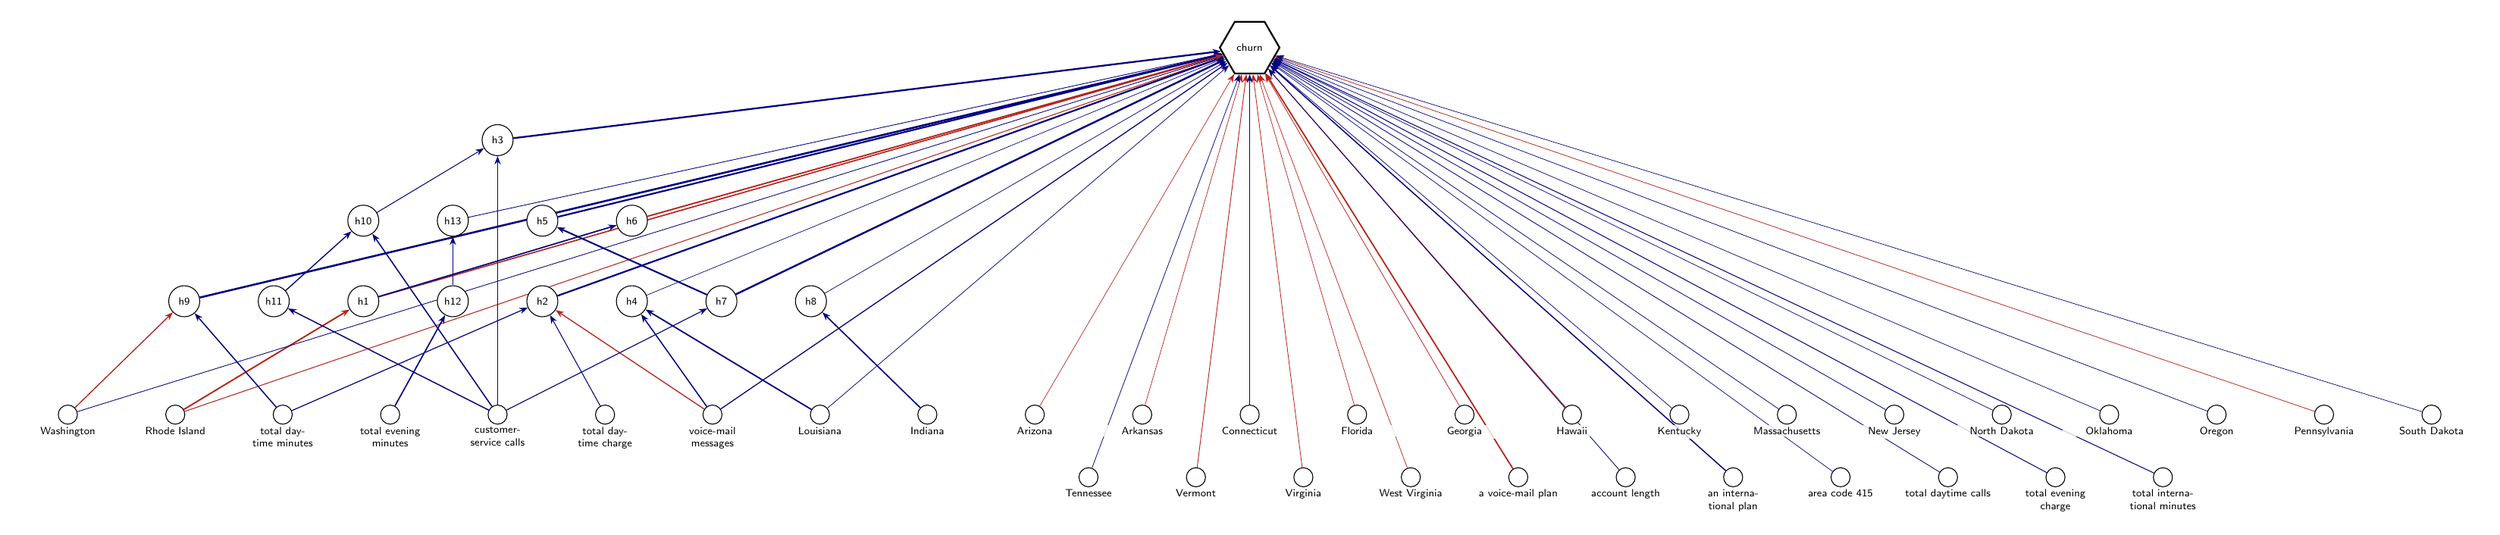
\begin{tikzpicture}[
  font=\sffamily\scriptsize, >={Stealth[length=1.4mm]},
  inp/.style={draw, circle, fill=white, minimum size=3.2mm, inner sep=0pt},
  hid/.style={draw, circle, fill=white, minimum size=5.2mm, inner sep=0.5pt, font=\sffamily\tiny},
  exitbox/.style={draw, thick, rectangle, fill=white, align=center, text width=17mm, minimum height=5mm, inner sep=1.5pt, font=\sffamily\tiny},
  sumbox/.style={draw, thick, dashed, rectangle, fill=white, align=center, text width=17mm, minimum height=5mm, inner sep=1.5pt, font=\sffamily\tiny},
  outp/.style={draw, thick, regular polygon, regular polygon sides=6, fill=white, minimum size=10mm, inner sep=0pt, font=\sffamily\tiny, align=center},
  stub/.style={draw, dashed, rounded corners=2pt, fill=white, align=center, inner sep=2pt, font=\sffamily\tiny, text width=15mm},
  inlab/.style={font=\sffamily\tiny, align=center, text width=15mm, inner sep=1pt, fill=white, fill opacity=0.8, text opacity=1},
  wpos/.style={draw=NavyBlue}, wneg/.style={draw=BrickRed}, wagg/.style={draw=black!45, line width=1.2pt},
  wmix/.style={draw=Plum},
]
\node[inp] (ninxxstatex17) at (27.0,0.0) {};
\path (ninxxstatex17.south) node[inlab, anchor=north] (labninxxstatex17) {Kentucky};
\node[inp] (ninxxstatex18) at (12.6,0.0) {};
\path (ninxxstatex18.south) node[inlab, anchor=north] (labninxxstatex18) {Louisiana};
\node[inp] (ninxxstatex19) at (28.8,0.0) {};
\path (ninxxstatex19.south) node[inlab, anchor=north] (labninxxstatex19) {Massachusetts};
\node[inp] (ninxxstatex2) at (18.0,0.0) {};
\path (ninxxstatex2.south) node[inlab, anchor=north] (labninxxstatex2) {Arkansas};
\node[inp] (ninxxstatex28) at (32.4,0.0) {};
\path (ninxxstatex28.south) node[inlab, anchor=north] (labninxxstatex28) {North Dakota};
\node[inp] (ninxxstatex3) at (16.2,0.0) {};
\path (ninxxstatex3.south) node[inlab, anchor=north] (labninxxstatex3) {Arizona};
\node[inp] (ninxxstatex31) at (30.6,0.0) {};
\path (ninxxstatex31.south) node[inlab, anchor=north] (labninxxstatex31) {New Jersey};
\node[inp] (ninxxstatex10) at (23.4,0.0) {};
\path (ninxxstatex10.south) node[inlab, anchor=north] (labninxxstatex10) {Georgia};
\node[inp] (ninxxstatex36) at (34.2,0.0) {};
\path (ninxxstatex36.south) node[inlab, anchor=north] (labninxxstatex36) {Oklahoma};
\node[inp] (ninxxstatex37) at (36.0,0.0) {};
\path (ninxxstatex37.south) node[inlab, anchor=north] (labninxxstatex37) {Oregon};
\node[inp] (ninxxstatex38) at (37.8,0.0) {};
\path (ninxxstatex38.south) node[inlab, anchor=north] (labninxxstatex38) {Pennsylvania};
\node[inp] (ninxxstatex39) at (1.8,0.0) {};
\path (ninxxstatex39.south) node[inlab, anchor=north] (labninxxstatex39) {Rhode Island};
\node[inp] (ninxxstatex41) at (39.6,0.0) {};
\path (ninxxstatex41.south) node[inlab, anchor=north] (labninxxstatex41) {South Dakota};
\node[inp] (ninxxstatex42) at (17.1,-1.05) {};
\path (ninxxstatex42.south) node[inlab, anchor=north] (labninxxstatex42) {Tennessee};
\node[inp] (ninxxstatex11) at (25.2,0.0) {};
\path (ninxxstatex11.south) node[inlab, anchor=north] (labninxxstatex11) {Hawaii};
\node[inp] (ninxxstatex45) at (20.7,-1.05) {};
\path (ninxxstatex45.south) node[inlab, anchor=north] (labninxxstatex45) {Virginia};
\node[inp] (ninxxstatex46) at (18.9,-1.05) {};
\path (ninxxstatex46.south) node[inlab, anchor=north] (labninxxstatex46) {Vermont};
\node[inp] (ninxxstatex47) at (0.0,0.0) {};
\path (ninxxstatex47.south) node[inlab, anchor=north] (labninxxstatex47) {Washington};
\node[inp] (ninxxstatex49) at (22.5,-1.05) {};
\path (ninxxstatex49.south) node[inlab, anchor=north] (labninxxstatex49) {West Virginia};
\node[inp] (ninxxstatex6) at (19.8,0.0) {};
\path (ninxxstatex6.south) node[inlab, anchor=north] (labninxxstatex6) {Connecticut};
\node[inp] (ninxxstatex9) at (21.6,0.0) {};
\path (ninxxstatex9.south) node[inlab, anchor=north] (labninxxstatex9) {Florida};
\node[inp] (ninxxaccountxlength) at (26.1,-1.05) {};
\path (ninxxaccountxlength.south) node[inlab, anchor=north] (labninxxaccountxlength) {account length};
\node[inp] (ninxxareaxcodex415) at (29.7,-1.05) {};
\path (ninxxareaxcodex415.south) node[inlab, anchor=north] (labninxxareaxcodex415) {area code 415};
\node[inp] (ninxxinternationalxplan) at (27.9,-1.05) {};
\path (ninxxinternationalxplan.south) node[inlab, anchor=north] (labninxxinternationalxplan) {an international plan};
\node[inp] (ninxxvoicexmailxplan) at (24.3,-1.05) {};
\path (ninxxvoicexmailxplan.south) node[inlab, anchor=north] (labninxxvoicexmailxplan) {a voice-mail plan};
\node[inp] (ninxxnumberxvmailxmessages) at (10.8,0.0) {};
\path (ninxxnumberxvmailxmessages.south) node[inlab, anchor=north] (labninxxnumberxvmailxmessages) {voice-mail messages};
\node[inp] (ninxxtotalxdayxminutes) at (3.6,0.0) {};
\path (ninxxtotalxdayxminutes.south) node[inlab, anchor=north] (labninxxtotalxdayxminutes) {total daytime minutes};
\node[inp] (ninxxtotalxdayxcalls) at (31.5,-1.05) {};
\path (ninxxtotalxdayxcalls.south) node[inlab, anchor=north] (labninxxtotalxdayxcalls) {total daytime calls};
\node[inp] (ninxxtotalxdayxcharge) at (9.0,0.0) {};
\path (ninxxtotalxdayxcharge.south) node[inlab, anchor=north] (labninxxtotalxdayxcharge) {total daytime charge};
\node[inp] (ninxxtotalxevexminutes) at (5.4,0.0) {};
\path (ninxxtotalxevexminutes.south) node[inlab, anchor=north] (labninxxtotalxevexminutes) {total evening minutes};
\node[inp] (ninxxtotalxevexcharge) at (33.3,-1.05) {};
\path (ninxxtotalxevexcharge.south) node[inlab, anchor=north] (labninxxtotalxevexcharge) {total evening charge};
\node[inp] (ninxxtotalxintlxminutes) at (35.1,-1.05) {};
\path (ninxxtotalxintlxminutes.south) node[inlab, anchor=north] (labninxxtotalxintlxminutes) {total international minutes};
\node[inp] (ninxxnumberxcustomerxservicexcalls) at (7.2,0.0) {};
\path (ninxxnumberxcustomerxservicexcalls.south) node[inlab, anchor=north] (labninxxnumberxcustomerxservicexcalls) {customer-service calls};
\node[inp] (ninxxstatex15) at (14.4,0.0) {};
\path (ninxxstatex15.south) node[inlab, anchor=north] (labninxxstatex15) {Indiana};
\node[outp] (n0) at (19.8,6.15) {churn};
\node[hid] (n10131) at (1.95,1.9) {h9};
\node[hid] (n12171) at (4.95,3.25) {h10};
\node[hid] (n12730) at (3.45,1.9) {h11};
\node[hid] (n1295) at (4.95,1.9) {h1};
\node[hid] (n14484) at (6.45,1.9) {h12};
\node[hid] (n15524) at (6.45,3.25) {h13};
\node[hid] (n3118) at (7.95,1.9) {h2};
\node[hid] (n5268) at (7.2,4.6) {h3};
\node[hid] (n6089) at (9.45,1.9) {h4};
\node[hid] (n6713) at (7.95,3.25) {h5};
\node[hid] (n7872) at (9.45,3.25) {h6};
\node[hid] (n9436) at (10.95,1.9) {h7};
\node[hid] (n9954) at (12.45,1.9) {h8};
\begin{scope}[on background layer]
\draw[->, wpos, line width=0.26pt] (ninxxstatex17) -- (n0);
\draw[->, wpos, line width=0.27pt] (ninxxstatex18) -- (n0);
\draw[->, wpos, line width=0.65pt] (ninxxstatex18) -- (n6089);
\draw[->, wpos, line width=0.27pt] (ninxxstatex19) -- (n0);
\draw[->, wneg, line width=0.26pt] (ninxxstatex2) -- (n0);
\draw[->, wpos, line width=0.25pt] (ninxxstatex28) -- (n0);
\draw[->, wneg, line width=0.25pt] (ninxxstatex3) -- (n0);
\draw[->, wpos, line width=0.29pt] (ninxxstatex31) -- (n0);
\draw[->, wneg, line width=0.28pt] (ninxxstatex10) -- (n0);
\draw[->, wpos, line width=0.25pt] (ninxxstatex36) -- (n0);
\draw[->, wpos, line width=0.26pt] (ninxxstatex37) -- (n0);
\draw[->, wneg, line width=0.28pt] (ninxxstatex38) -- (n0);
\draw[->, wneg, line width=0.38pt] (ninxxstatex39) -- (n0);
\draw[->, wneg, line width=0.69pt] (ninxxstatex39) -- (n1295);
\draw[->, wpos, line width=0.25pt] (ninxxstatex41) -- (n0);
\draw[->, wpos, line width=0.27pt] (ninxxstatex42) -- (n0);
\draw[->, wneg, line width=0.38pt] (ninxxstatex11) -- (n0);
\draw[->, wneg, line width=0.30pt] (ninxxstatex45) -- (n0);
\draw[->, wneg, line width=0.34pt] (ninxxstatex46) -- (n0);
\draw[->, wpos, line width=0.31pt] (ninxxstatex47) -- (n0);
\draw[->, wneg, line width=0.49pt] (ninxxstatex47) -- (n10131);
\draw[->, wneg, line width=0.27pt] (ninxxstatex49) -- (n0);
\draw[->, wpos, line width=0.27pt] (ninxxstatex6) -- (n0);
\draw[->, wneg, line width=0.26pt] (ninxxstatex9) -- (n0);
\draw[->, wpos, line width=0.29pt] (ninxxaccountxlength) -- (n0);
\draw[->, wpos, line width=0.25pt] (ninxxareaxcodex415) -- (n0);
\draw[->, wpos, line width=0.54pt] (ninxxinternationalxplan) -- (n0);
\draw[->, wneg, line width=0.64pt] (ninxxvoicexmailxplan) -- (n0);
\draw[->, wpos, line width=0.47pt] (ninxxnumberxvmailxmessages) -- (n0);
\draw[->, wneg, line width=0.48pt] (ninxxnumberxvmailxmessages) -- (n3118);
\draw[->, wpos, line width=0.54pt] (ninxxnumberxvmailxmessages) -- (n6089);
\draw[->, wpos, line width=0.54pt] (ninxxtotalxdayxminutes) -- (n10131);
\draw[->, wpos, line width=0.44pt] (ninxxtotalxdayxminutes) -- (n3118);
\draw[->, wpos, line width=0.30pt] (ninxxtotalxdayxcalls) -- (n0);
\draw[->, wpos, line width=0.38pt] (ninxxtotalxdayxcharge) -- (n3118);
\draw[->, wpos, line width=0.60pt] (ninxxtotalxevexminutes) -- (n14484);
\draw[->, wpos, line width=0.37pt] (ninxxtotalxevexcharge) -- (n0);
\draw[->, wpos, line width=0.37pt] (ninxxtotalxintlxminutes) -- (n0);
\draw[->, wpos, line width=0.55pt] (ninxxnumberxcustomerxservicexcalls) -- (n12171);
\draw[->, wpos, line width=0.53pt] (ninxxnumberxcustomerxservicexcalls) -- (n12730);
\draw[->, wpos, line width=0.34pt] (ninxxnumberxcustomerxservicexcalls) -- (n5268);
\draw[->, wpos, line width=0.41pt] (ninxxnumberxcustomerxservicexcalls) -- (n9436);
\draw[->, wpos, line width=0.60pt] (ninxxstatex15) -- (n9954);
\draw[->, wpos, line width=0.92pt] (n10131) -- (n0);
\draw[->, wpos, line width=0.38pt] (n12171) -- (n5268);
\draw[->, wpos, line width=0.50pt] (n12730) -- (n12171);
\draw[->, wneg, line width=0.60pt] (n1295) -- (n0);
\draw[->, wpos, line width=0.61pt] (n1295) -- (n7872);
\draw[->, wpos, line width=0.61pt] (n14484) -- (n15524);
\draw[->, wpos, line width=0.32pt] (n15524) -- (n0);
\draw[->, wpos, line width=0.79pt] (n3118) -- (n0);
\draw[->, wpos, line width=0.83pt] (n5268) -- (n0);
\draw[->, wpos, line width=0.25pt] (n6089) -- (n0);
\draw[->, wpos, line width=0.79pt] (n6713) -- (n0);
\draw[->, wneg, line width=0.67pt] (n7872) -- (n0);
\draw[->, wpos, line width=0.87pt] (n9436) -- (n0);
\draw[->, wpos, line width=0.75pt] (n9436) -- (n6713);
\draw[->, wpos, line width=0.26pt] (n9954) -- (n0);
\end{scope}
\end{tikzpicture}}%
\caption{The network as trained, before any explanation, in full. Blue: positive weight (raises the score); red: negative weight (lowers it); thicker: larger weight. Orange outline and up arrow: raises the final prediction; teal and down arrow: lowers it; grey and double arrow: depends. Not used (no connection): Alaska, Alabama, Iowa, Idaho, Illinois, Kansas, Maryland, Maine, Michigan, Minnesota, Missouri, Mississippi, Montana, North Carolina, Nebraska, New Hampshire, New Mexico, Nevada, New York, Ohio, California, South Carolina, Texas, Utah, Wisconsin, Colorado, Wyoming, Washington DC, Delaware, area code 408, area code 510, total evening calls, total night-time minutes, total night-time calls, total night-time charge, total international calls, total international charge.}
\label{fig:churn100s4c2:raw}
\end{figure}
\end{landscape}
\end{drafted}
\clearpage
\end{document}
